% !TeX spellcheck = en_GB
% !TeX encoding = UTF-8
% !TeX program = xelatex
% TODO Change language to en_GB (recommended) or en_US for English documents
%\documentclass[11pt,a4paper,oneside]{report}             % Single-side
\documentclass[11pt,a4paper,twoside,openright]{report}  % Duplex

% thanks to http://tex.stackexchange.com/a/47579/71109
\usepackage{ifxetex}
\usepackage{ifluatex}
\newif\ifxetexorluatex % a new conditional starts as false
\ifnum 0\ifxetex 1\fi\ifluatex 1\fi>0
   \xetexorluatextrue
\fi

\ifxetexorluatex
  \usepackage{fontspec}
\else
  \usepackage[T1]{fontenc}
  \usepackage[utf8]{inputenc}
  \usepackage[lighttt]{lmodern}
\fi

\usepackage[english,magyar]{babel} % Alapértelmezés szerint utoljára definiált nyelv lesz aktív, de később külön beállítjuk az aktív nyelvet.

%\usepackage{cmap}
\usepackage{amsfonts,amsmath,amssymb} % Mathematical symbols.
%\usepackage[ruled,boxed,resetcount,linesnumbered]{algorithm2e} % For pseudocodes. % beware: this is not compatible with LuaLaTeX, see http://tex.stackexchange.com/questions/34814/lualatex-and-algorithm2e
\usepackage{booktabs} % For publication quality tables for LaTeX
\usepackage{graphicx}

%\usepackage{fancyhdr}
%\usepackage{lastpage}

\usepackage{anysize}
%\usepackage{sectsty}
\usepackage{setspace} % For setting line spacing

\usepackage[unicode]{hyperref} % For hyperlinks in the generated document.
\usepackage{xcolor}
\usepackage{listings} % For source code snippets.

\usepackage[amsmath,thmmarks]{ntheorem} % Theorem-like environments.

\usepackage[hang]{caption}

\singlespacing

\newcommand{\selecthungarian}{
	\selectlanguage{magyar}
	\setlength{\parindent}{2em}
	\setlength{\parskip}{0em}
	\frenchspacing
}

\newcommand{\selectenglish}{
	\selectlanguage{english}
	\setlength{\parindent}{0em}
	\setlength{\parskip}{0.5em}
	\nonfrenchspacing
	\renewcommand{\figureautorefname}{Figure}
	\renewcommand{\tableautorefname}{Table}
	\renewcommand{\partautorefname}{Part}
	\renewcommand{\chapterautorefname}{Chapter}
	\renewcommand{\sectionautorefname}{Section}
	\renewcommand{\subsectionautorefname}{Section}
	\renewcommand{\subsubsectionautorefname}{Section}
}

\usepackage[numbers]{natbib}
\usepackage{xspace}


%TODO Set the main variables
\newcommand{\vikszerzoVezeteknev}{Debreczeni}
\newcommand{\vikszerzoKeresztnev}{László}

\newcommand{\vikkonzulensAMegszolitas}{}
\newcommand{\vikkonzulensAVezeteknev}{Sörös (Nokia)}
\newcommand{\vikkonzulensAKeresztnev}{Gábor}

\newcommand{\vikkonzulensBMegszolitas}{}
\newcommand{\vikkonzulensBVezeteknev}{Tevesz}
\newcommand{\vikkonzulensBKeresztnev}{Judit}

\newcommand{\vikkonzulensCMegszolitas}{}
\newcommand{\vikkonzulensCVezeteknev}{}
\newcommand{\vikkonzulensCKeresztnev}{}

\newcommand{\vikcim}{Environment mapping with a mobile robot} % Cím
\newcommand{\viktanszek}{\bmeaut} % Tanszék
\newcommand{\vikdoktipus}{\msc} % Dokumentum típusa (\bsc vagy \msc)
\newcommand{\vikmunkatipusat}{diplomatervet} % a "hallgató nyilatkozat" részhez: szakdolgozatot vagy diplomatervet

%--------------------------------------------------------------------------------------
% TDK-specifikus változók
%--------------------------------------------------------------------------------------
\newcommand{\tdkszerzoB}{Második Szerző} % Második szerző neve; hagyd üresen, ha egyedül írtad a TDK-t.
\newcommand{\tdkev}{2014} % A dolgozat írásának éve (pl. "2014") (Ez OTDK-nál eltérhet az aktuális évtől.)

% További adatok az OTDK címlaphoz (BME-s TDK-hoz nem kell kitölteni)
\newcommand{\tdkevfolyamA}{IV} % Első szerző évfolyama, római számmal (pl. IV).
\newcommand{\tdkevfolyamB}{III} % Második szerző évfolyama, római számmal (pl. III).
\newcommand{\tdkkonzulensbeosztasA}{egyetemi tanár} % Első konzulens beosztása (pl. egyetemi docens)
\newcommand{\tdkkonzulensbeosztasB}{doktorandusz} % Második konzulens beosztása (pl. egyetemi docens)

\newcommand{\szerzoMeta}{\vikszerzoVezeteknev{} \vikszerzoKeresztnev} % egy szerző esetén
%\newcommand{\szerzoMeta}{\vikszerzoVezeteknev{} \vikszerzoKeresztnev, \tdkszerzoB} % két szerző esetén

%TODO Language configuration -- choose one
% Beállítások magyar nyelvű dolgozathoz
%%--------------------------------------------------------------------------------------
% Elnevezések
%--------------------------------------------------------------------------------------
\newcommand{\bme}{Budapesti Műszaki és Gazdaságtudományi Egyetem}
\newcommand{\vik}{Villamosmérnöki és Informatikai Kar}

\newcommand{\bmemit}{Méréstechnika és Információs Rendszerek Tanszék}

\newcommand{\keszitette}{Készítette}
\newcommand{\konzulens}{Konzulens}

\newcommand{\bsc}{Szakdolgozat}
\newcommand{\msc}{Diplomaterv}
\newcommand{\tdk}{TDK dolgozat}
\newcommand{\bsconlab}{BSc Önálló laboratórium}
\newcommand{\msconlabi}{MSc Önálló laboratórium 1.}
\newcommand{\msconlabii}{MSc Önálló laboratórium 2.}

\newcommand{\pelda}{Példa}
\newcommand{\definicio}{Definíció}
\newcommand{\tetel}{Tétel}

\newcommand{\bevezetes}{Bevezetés}
\newcommand{\koszonetnyilvanitas}{Köszönetnyilvánítás}
\newcommand{\fuggelek}{Függelék}

% Opcionálisan átnevezhető címek
%\addto\captionsmagyar{%
%\renewcommand{\listfigurename}{Saját ábrajegyzék cím}
%\renewcommand{\listtablename}{Saját táblázatjegyzék cím}
%\renewcommand{\bibname}{Saját irodalomjegyzék név}
%}

\newcommand{\szerzo}{\vikszerzoVezeteknev{} \vikszerzoKeresztnev}
\newcommand{\vikkonzulensA}{\vikkonzulensAMegszolitas\vikkonzulensAVezeteknev{} \vikkonzulensAKeresztnev}
\newcommand{\vikkonzulensB}{\vikkonzulensBMegszolitas\vikkonzulensBVezeteknev{} \vikkonzulensBKeresztnev}
\newcommand{\vikkonzulensC}{\vikkonzulensCMegszolitas\vikkonzulensCVezeteknev{} \vikkonzulensCKeresztnev}

\newcommand{\selectthesislanguage}{\selecthungarian}

\bibliographystyle{huplain}

\def\lstlistingname{lista}

\newcommand{\appendixnumber}{6}  % a fofejezet-szamlalo az angol ABC 6. betuje (F) lesz

% Settings for English documents
%--------------------------------------------------------------------------------------
% Elnevezések
%--------------------------------------------------------------------------------------
\newcommand{\bme}{Budapest University of Technology and Economics}
\newcommand{\vik}{Faculty of Electrical Engineering and Informatics}

\newcommand{\bmemit}{Department of Measurement and Information Systems}
\newcommand{\bmeaut}{Department of Automation and Applied Informatics}

\newcommand{\keszitette}{Author}
\newcommand{\konzulens}{Advisor}

\newcommand{\bsc}{Bachelor's Thesis}
\newcommand{\msc}{Master's Thesis}
\newcommand{\tdk}{Scientific Students' Association Report}
\newcommand{\bsconlab}{BSc Project Laboratory}
\newcommand{\msconlabi}{MSc Project Laboratory 1}
\newcommand{\msconlabii}{MSc Project Laboratory 2}

\newcommand{\pelda}{Example}
\newcommand{\definicio}{Definition}
\newcommand{\tetel}{Theorem}

\newcommand{\bevezetes}{Introduction}
\newcommand{\koszonetnyilvanitas}{Acknowledgements}
\newcommand{\fuggelek}{Appendix}

% Optional custom titles
%\addto\captionsenglish{%
%\renewcommand*{\listfigurename}{Your list of figures title}
%\renewcommand*{\listtablename}{Your list of tables title}
%\renewcommand*{\bibname}{Your bibliography title}
%}

\newcommand{\szerzo}{\vikszerzoKeresztnev{} \vikszerzoVezeteknev}
\newcommand{\vikkonzulensA}{\vikkonzulensAMegszolitas\vikkonzulensAKeresztnev{} \vikkonzulensAVezeteknev}
\newcommand{\vikkonzulensB}{\vikkonzulensBMegszolitas\vikkonzulensBKeresztnev{} \vikkonzulensBVezeteknev}
\newcommand{\vikkonzulensC}{\vikkonzulensCMegszolitas\vikkonzulensCKeresztnev{} \vikkonzulensCVezeteknev}

\newcommand{\selectthesislanguage}{\selectenglish}

\bibliographystyle{plainnat}

\newcommand{\ie}{i.e.\@\xspace}
\newcommand{\Ie}{I.e.\@\xspace}
\newcommand{\eg}{e.g.\@\xspace}
\newcommand{\Eg}{E.g.\@\xspace}
\newcommand{\etal}{et al.\@\xspace}
\newcommand{\etc}{etc.\@\xspace}
\newcommand{\vs}{vs.\@\xspace}
\newcommand{\viz}{viz.\@\xspace} % videlicet
\newcommand{\cf}{cf.\@\xspace} % confer
\newcommand{\Cf}{Cf.\@\xspace}
\newcommand{\wrt}{w.r.t.\@\xspace} % with respect to
\newcommand{\approximately}{approx.\@\xspace}

\newcommand{\appendixnumber}{1}  % a fofejezet-szamlalo az angol ABC 1. betuje (A) lesz


%--------------------------------------------------------------------------------------
% Page layout setup
%--------------------------------------------------------------------------------------
% we need to redefine the pagestyle plain
% another possibility is to use the body of this command without \fancypagestyle
% and use \pagestyle{fancy} but in that case the special pages
% (like the ToC, the References, and the Chapter pages)remain in plane style

\pagestyle{plain}
\marginsize{35mm}{25mm}{15mm}{15mm}

\setcounter{tocdepth}{3}
%\sectionfont{\large\upshape\bfseries}
\setcounter{secnumdepth}{3}

\sloppy % Margón túllógó sorok tiltása.
\widowpenalty=10000 \clubpenalty=10000 %A fattyú- és árvasorok elkerülése
\def\hyph{-\penalty0\hskip0pt\relax} % Kötőjeles szavak elválasztásának engedélyezése


%--------------------------------------------------------------------------------------
% Setup hyperref package
%--------------------------------------------------------------------------------------
\hypersetup{
    % bookmarks=true,            % show bookmarks bar?
    unicode=true,              % non-Latin characters in Acrobat's bookmarks
    pdftitle={\vikcim},        % title
    pdfauthor={\szerzoMeta},    % author
    pdfsubject={\vikdoktipus}, % subject of the document
    pdfcreator={\szerzoMeta},   % creator of the document
    pdfproducer={},    % producer of the document
    pdfkeywords={},    % list of keywords (separate then by comma)
    pdfnewwindow=true,         % links in new window
    colorlinks=true,           % false: boxed links; true: colored links
    linkcolor=black,           % color of internal links
    citecolor=black,           % color of links to bibliography
    filecolor=black,           % color of file links
    urlcolor=black             % color of external links
}


%--------------------------------------------------------------------------------------
% Set up listings
%--------------------------------------------------------------------------------------
\definecolor{lightgray}{rgb}{0.95,0.95,0.95}
\lstset{
	basicstyle=\scriptsize\ttfamily, % print whole listing small
	keywordstyle=\color{black}\bfseries, % bold black keywords
	identifierstyle=, % nothing happens
	% default behavior: comments in italic, to change use
	% commentstyle=\color{green}, % for e.g. green comments
	stringstyle=\scriptsize,
	showstringspaces=false, % no special string spaces
	aboveskip=3pt,
	belowskip=3pt,
	backgroundcolor=\color{lightgray},
	columns=flexible,
	keepspaces=true,
	escapeinside={(*@}{@*)},
	captionpos=b,
	breaklines=true,
	frame=single,
	float=!ht,
	tabsize=2,
	literate=*
		{á}{{\'a}}1	{é}{{\'e}}1	{í}{{\'i}}1	{ó}{{\'o}}1	{ö}{{\"o}}1	{ő}{{\H{o}}}1	{ú}{{\'u}}1	{ü}{{\"u}}1	{ű}{{\H{u}}}1
		{Á}{{\'A}}1	{É}{{\'E}}1	{Í}{{\'I}}1	{Ó}{{\'O}}1	{Ö}{{\"O}}1	{Ő}{{\H{O}}}1	{Ú}{{\'U}}1	{Ü}{{\"U}}1	{Ű}{{\H{U}}}1
}


%--------------------------------------------------------------------------------------
% Set up theorem-like environments
%--------------------------------------------------------------------------------------
% Using ntheorem package -- see http://www.math.washington.edu/tex-archive/macros/latex/contrib/ntheorem/ntheorem.pdf

\theoremstyle{plain}
\theoremseparator{.}
\newtheorem{example}{\pelda}

\theoremseparator{.}
%\theoremprework{\bigskip\hrule\medskip}
%\theorempostwork{\hrule\bigskip}
\theorembodyfont{\upshape}
\theoremsymbol{{\large \ensuremath{\centerdot}}}
\newtheorem{definition}{\definicio}

\theoremseparator{.}
%\theoremprework{\bigskip\hrule\medskip}
%\theorempostwork{\hrule\bigskip}
\newtheorem{theorem}{\tetel}


%--------------------------------------------------------------------------------------
% Some new commands and declarations
%--------------------------------------------------------------------------------------
\newcommand{\code}[1]{{\upshape\ttfamily\scriptsize\indent #1}}
\newcommand{\doi}[1]{DOI: \href{http://dx.doi.org/\detokenize{#1}}{\raggedright{\texttt{\detokenize{#1}}}}} % A hivatkozások közt így könnyebb DOI-t megadni.

\DeclareMathOperator*{\argmax}{arg\,max}
%\DeclareMathOperator*[1]{\floor}{arg\,max}
\DeclareMathOperator{\sign}{sgn}
\DeclareMathOperator{\rot}{rot}


%--------------------------------------------------------------------------------------
% Setup captions
%--------------------------------------------------------------------------------------
\captionsetup[figure]{
	width=.75\textwidth,
	aboveskip=10pt}

\renewcommand{\captionlabelfont}{\bf}
%\renewcommand{\captionfont}{\footnotesize\it}

%--------------------------------------------------------------------------------------
% Hyphenation exceptions
%--------------------------------------------------------------------------------------
\hyphenation{Shakes-peare Mar-seilles ár-víz-tű-rő tü-kör-fú-ró-gép}


\author{\vikszerzo}
\title{\viktitle}


\usepackage{enumitem} % this is needed for reducing the space betwen enumeration items
\newcommand{\LD}[1]{\textcolor{cyan}{GH: \em#1}}
\newcommand{\GS}[1]{\textcolor{orange}{GS: \em#1}}


%--------------------------------------------------------------------------------------
% Table of contents and the main text
%--------------------------------------------------------------------------------------
\begin{document}

\pagenumbering{gobble}

%TODO These includes define guidelines -- remove these
%~~~~~~~~~~~~~~~~~~~~~~~~~~~~~~~~~~~~~~~~~~~~~~~~~~~~~~~~~~~~~~~~~~~~~~~~~~~~~~~~~~~~~~
%\selecthungarian
%--------------------------------------------------------------------------------------
% Rovid formai es tartalmi tajekoztato
%--------------------------------------------------------------------------------------

\footnotesize
\begin{center}
\large
\textbf{\Large Általános információk, a diplomaterv szerkezete}\\
\end{center}

A diplomaterv szerkezete a BME Villamosmérnöki és Informatikai Karán:
\begin{enumerate}
\item	Diplomaterv feladatkiírás
\item	Címoldal
\item	Tartalomjegyzék
\item	A diplomatervező nyilatkozata az önálló munkáról és az elektronikus adatok kezeléséről
\item	Tartalmi összefoglaló magyarul és angolul
\item	Bevezetés: a feladat értelmezése, a tervezés célja, a feladat indokoltsága, a diplomaterv felépítésének rövid összefoglalása
\item	A feladatkiírás pontosítása és részletes elemzése
\item	Előzmények (irodalomkutatás, hasonló alkotások), az ezekből levonható következtetések
\item	A tervezés részletes leírása, a döntési lehetőségek értékelése és a választott megoldások indoklása
\item	A megtervezett műszaki alkotás értékelése, kritikai elemzése, továbbfejlesztési lehetőségek
\item	Esetleges köszönetnyilvánítások
\item	Részletes és pontos irodalomjegyzék
\item	Függelék(ek)
\end{enumerate}

Felhasználható a következő oldaltól kezdődő \LaTeX diplomatervsablon dokumentum tartalma. 

A diplomaterv szabványos méretű A4-es lapokra kerüljön. Az oldalak tükörmargóval készüljenek (mindenhol 2,5~cm, baloldalon 1~cm-es kötéssel). Az alapértelmezett betűkészlet a 12 pontos Times New Roman, másfeles sorközzel, de ettől kismértékben el lehet térni, ill. más betűtípus használata is megengedett.

Minden oldalon -- az első négy szerkezeti elem kivételével -- szerepelnie kell az oldalszámnak.

A fejezeteket decimális beosztással kell ellátni. Az ábrákat a megfelelő helyre be kell illeszteni, fejezetenként decimális számmal és kifejező címmel kell ellátni. A fejezeteket decimális aláosztással számozzuk, maximálisan 3 aláosztás mélységben (pl. 2.3.4.1.). Az ábrákat, táblázatokat és képleteket célszerű fejezetenként külön számozni (pl. 2.4. ábra, 4.2. táblázat vagy képletnél (3.2)). A fejezetcímeket igazítsuk balra, a normál szövegnél viszont használjunk sorkiegyenlítést. Az ábrákat, táblázatokat és a hozzájuk tartozó címet igazítsuk középre. A cím a jelölt rész alatt helyezkedjen el.

A képeket lehetőleg rajzoló programmal készítsék el, az egyenleteket egyenlet-szerkesztő segítségével írják le (A \LaTeX~ehhez kézenfekvő megoldásokat nyújt).

Az irodalomjegyzék szövegközi hivatkozása történhet sorszámozva (ez a preferált megoldás) vagy a Harvard-rendszerben (a szerző és az évszám megadásával). A teljes lista névsor szerinti sorrendben a szöveg végén szerepeljen (sorszámozott irodalmi hivatkozások esetén hivatkozási sorrendben). A szakirodalmi források címeit azonban mindig az eredeti nyelven kell megadni, esetleg zárójelben a fordítással. A listában szereplő valamennyi publikációra hivatkozni kell a szövegben (a \LaTeX-sablon a Bib\TeX~segítségével mindezt automatikusan kezeli). Minden publikáció a szerzők után a következő adatok szerepelnek: folyóirat cikkeknél a pontos cím, a folyóirat címe, évfolyam, szám, oldalszám tól-ig. A folyóiratok címét csak akkor rövidítsük, ha azok nagyon közismertek vagy nagyon hosszúak. Internetes hivatkozások megadásakor fontos, hogy az elérési út előtt megadjuk az oldal tulajdonosát és tartalmát (mivel a link egy idő után akár elérhetetlenné is válhat), valamint az elérés időpontját.

\vspace{5mm}
Fontos:
\begin{itemize}
	\item A szakdolgozatkészítő / diplomatervező nyilatkozata (a jelen sablonban szereplő szövegtartalommal) kötelező előírás, Karunkon ennek hiányában a szakdolgozat/diplomaterv nem bírálható és nem védhető!
	\item Mind a dolgozat, mind a melléklet maximálisan 15~MB méretű lehet!
\end{itemize}

\vspace{5mm}
\begin{center}
Jó munkát, sikeres szakdolgozatkészítést, ill. diplomatervezést kívánunk!
\end{center}

\normalsize
\selectthesislanguage

%%--------------------------------------------------------------------------------------
% Feladatkiiras (a tanszeken atveheto, kinyomtatott valtozat)
%--------------------------------------------------------------------------------------
\clearpage
\begin{center}
\large
\textbf{FELADATKIÍRÁS}\\
\end{center}

A feladatkiírást a tanszéki adminisztrációban lehet átvenni, és a leadott munkába eredeti, tanszéki pecséttel ellátott és a tanszékvezető által aláírt lapot kell belefűzni (ezen oldal \emph{helyett}, ez az oldal csak útmutatás). Az elektronikusan feltöltött dolgozatban már nem kell beleszerkeszteni ezt a feladatkiírást.


\selectthesislanguage

%TODO Titlepage -- choose one from below
%~~~~~~~~~~~~~~~~~~~~~~~~~~~~~~~~~~~~~~~~~~~~~~~~~~~~~~~~~~~~~~~~~~~~~~~~~~~~~~~~~~~~~~
\hypersetup{pageanchor=false}
%--------------------------------------------------------------------------------------
%	The title page
%--------------------------------------------------------------------------------------
\begin{titlepage}
\begin{center}

\includegraphics[width=60mm,keepaspectratio]{figures/bme_logo.pdf}\\
\vspace{0.3cm}
\textbf{\bme}\\
\textmd{\vik}\\
\textmd{\viktanszek}\\[5cm]

\vspace{0.4cm}
{\huge \bfseries \vikcim}\\[0.8cm]
\vspace{0.5cm}
\textsc{\Large \vikdoktipus}\\[4cm]

{
	\renewcommand{\arraystretch}{0.85}
	\begin{tabular}{cc}
	 \makebox[7cm]{\emph{\keszitette}} & \makebox[7cm]{\emph{\konzulens}} \\ \noalign{\smallskip}
	 \makebox[7cm]{\szerzo} & \makebox[7cm]{\vikkonzulensA} \\
	  & \makebox[7cm]{\vikkonzulensB} \\
	  & \makebox[7cm]{\vikkonzulensC} \\
	\end{tabular}
}

\vfill
{\large \today}
\end{center}
\end{titlepage}
\hypersetup{pageanchor=false}

		   % Szakdolgozat/Diplomaterv címlap
%%% TDK címlap
\begin{titlepage}
  \begin{center}  
  
\includegraphics[width=7cm]{./figures/bme_logo.pdf}
  \vspace{0.3cm}
  
  \bme \\
  \vik \\
  \viktanszek \\
  \vspace{5cm}
  
  \huge {\vikcim}
  \vspace{1.5cm}
  
  \large {\textbf{\tdk}}
  \vfill
    
  {\Large 
  	\keszitette: \\ \vspace{0.3cm}
  	\szerzo \\
	\tdkszerzoB \\
  	\vspace{1.5cm}
  	\konzulens: \\ \vspace{0.3cm}
  	\vikkonzulensA \\
  	\vikkonzulensB \\
  }
  
  \vspace{2cm}
  \large {\tdkev}
 \end{center}
\end{titlepage}
%% Címlap vége
	% TDK címlap
%%% OTDK külső címlap
\begin{titlepage}
  	$\;$ 
	\vspace{5cm}
	
	\begin{center}
	\Huge
	\textbf{TDK-dolgozat}\let\thefootnote\relax\footnote{A dolgozat bemutatását a XXXXXXXXX  ``Lorem ipsum dolor sit amet'' című program támogatta.}
	\end{center}
	
	\vspace{13cm}
	
	\Large
	\hspace{8cm} \szerzo
	
	\hspace{8cm} \tdkszerzoB
	
	\hspace{8cm} \tdkev.
\end{titlepage}

\newpage
\thispagestyle{empty}


%% OTDK belső címlap
\begin{titlepage}
  \begin{center}  
  
\includegraphics[width=7cm]{./figures/bme_logo.pdf}
  \vspace{0.3cm}
  
  \bme \\
  \vik \\
  \viktanszek \\
  \vspace{3.5cm}
  
  \huge {\vikcim}
  \vspace{1.5cm}
  
  \large {\textbf{\vikdoktipus}}
  \vfill
    
  {\Large 
  	{\large \keszitette:} \\ \vspace{0.2cm}
  	\szerzo \\ \tdkevfolyamA. évfolyam \\
	\vspace{0.5cm}
	\tdkszerzoB \\ \tdkevfolyamB. évfolyam \\
  	\vspace{1.5cm}
  	{\large \konzulens:} \\ \vspace{0.2cm}
  	\vikkonzulensA,\\ \tdkkonzulensbeosztasA \\
  	\vspace{0.5cm}
  	\vikkonzulensB,\\ \tdkkonzulensbeosztasB \\
  }
  
  \vspace{2cm}
  \large {\tdkev.}
  
 \end{center}
\end{titlepage}   % OTDK címlap


% Table of Contents
%~~~~~~~~~~~~~~~~~~~~~~~~~~~~~~~~~~~~~~~~~~~~~~~~~~~~~~~~~~~~~~~~~~~~~~~~~~~~~~~~~~~~~~
\tableofcontents\vfill


% Declaration and Abstract
%~~~~~~~~~~~~~~~~~~~~~~~~~~~~~~~~~~~~~~~~~~~~~~~~~~~~~~~~~~~~~~~~~~~~~~~~~~~~~~~~~~~~~~
\selectlanguage{magyar}
\pagenumbering{gobble}
%--------------------------------------------------------------------------------------
% Nyilatkozat
%--------------------------------------------------------------------------------------
\begin{center}
\large
\textbf{HALLGATÓI NYILATKOZAT}\\
\end{center}

Alulírott \emph{\vikszerzoVezeteknev{} \vikszerzoKeresztnev}, szigorló hallgató kijelentem, hogy ezt a \vikmunkatipusat{} meg nem engedett segítség nélkül, saját magam készítettem, csak a megadott forrásokat (szakirodalom, eszközök stb.) használtam fel. Minden olyan részt, melyet szó szerint, vagy azonos értelemben, de átfogalmazva más forrásból átvettem, egyértelműen, a forrás megadásával megjelöltem.

Hozzájárulok, hogy a jelen munkám alapadatait (szerző(k), cím, angol és magyar nyelvű tartalmi kivonat, készítés éve, konzulens(ek) neve) a BME VIK nyilvánosan hozzáférhető elektronikus formában, a munka teljes szövegét pedig az egyetem belső hálózatán keresztül (vagy autentikált felhasználók számára) közzétegye. Kijelentem, hogy a benyújtott munka és annak elektronikus verziója megegyezik. Dékáni engedéllyel titkosított diplomatervek esetén a dolgozat szövege csak 3 év eltelte után válik hozzáférhetővé.

\begin{flushleft}
\vspace*{1cm}
Budapest, \today
\end{flushleft}

\begin{flushright}
 \vspace*{1cm}
 \makebox[7cm]{\rule{6cm}{.4pt}}\\
 \makebox[7cm]{\emph{\vikszerzoVezeteknev{} \vikszerzoKeresztnev}}\\
 \makebox[7cm]{hallgató}
\end{flushright}
\thispagestyle{empty}

\vfill
\clearpage
\thispagestyle{empty} % an empty page

\selectthesislanguage
 %TODO Hallgatói nyilatkozat -- TDK és OTDK esetén törlendő!
\pagenumbering{roman}
\setcounter{page}{1}

\selecthungarian

%----------------------------------------------------------------------------
% Abstract in Hungarian
%----------------------------------------------------------------------------
\chapter*{Kivonat}\addcontentsline{toc}{chapter}{Kivonat}

Jelenleg az iparban egyre fontosabb szerepet töltenek be a mobilis robotok. Egyik legelterjedtebb felhasználásuk raktári környezetben történik, ahol képesek különböző rakományok szállítására. Ehhez első körben szükséges a környezet feltérképezése, mely manapság egy rendkívül gyakran kutatott téma, a robotika gyorsan fejlődő szegmense.

A feltérképezés alapvető eszközei a LiDAR-ok illetve különböző mélységi kamerák. LiDAR-ból létezik 2D-s és 3D-s változat, ugyanakkor az utóbbit ritkán alkalmazzák magas ára miatt. Amennyiben 3D-s feltérképezést szeretnénk használni (amely sokkal több területen alkalmazható), érdemesebb inkább valamilyen mélységi kamerát használnunk. Ez lehet RGB-D vagy sztereó. Ezen kamerák használatával nem csupán pontfelhőt tudunk felépíteni a környezetünkről, hanem akár képesek lehetünk különböző objektumok detektálására is. Ez azért fontos, mert egy raktárban szükség lehet emberek kikerülésére, illetve követésére.

Ezen diplomamunka megírása során a feladatom megvizsgálni, milyen módon alkalmazhatunk mélységi kamerákat mobilis robotokon környezetfeltérképezésre,  objektumfelismerésre, valamint fotorealisztikus környezeti rekonstrukcióra. A feltérképezés közben, illetve utána,  tájékozódás közben is cél a felismert személyeket kikerülni, illetve követni a robottal. Jelen munkát a Nokia Bell Labs-nél végeztem Budapesten, ahol lehetőségem nyílt a munkámat egy Turtlebot4 roboton tesztelni. A roboton található egy OAK-D Pro kamera, amelynek segítségével elvégeztem a feltérképezést. Célunknak tekintettük továbbá egy neurális rekonstrukció megvalósítását (\textit{NeRF} vagy \textit{Gaussian Splatting} segítségével) a feltérképezett környezetről, hogy fotorealisztikus modellt kapjunk a robotról és a környezetéről.


\vfill
\selectenglish


%----------------------------------------------------------------------------
% Abstract in English
%----------------------------------------------------------------------------
\chapter*{Abstract}\addcontentsline{toc}{chapter}{Abstract}
Currently, mobile robots play an increasingly important role in industry. One of their most common uses is in a warehouse environment, where they can transport different loads. This first requires mapping the environment, which is a frequently researched topic these days and a rapidly developing segment of robotics.

The basic tools for mapping are LiDARs and various depth cameras. There are 2D and 3D versions of LiDAR, but the latter is rarely used due to its high price. If we want to use 3D mapping (which promises much more possibilities), it is better to use some kind of depth camera. This can be RGB-D or stereo. By using these cameras, we can not only build a point cloud of our surroundings, but also be able to detect different objects around us. This is important because it may be necessary to avoid or follow people in a warehouse.

My task is to investigate how we can use depth cameras on mobile robots for environmental mapping, object detection, and photorealistic environment reconstruction. During operation, my aim is to avoid/follow the recognized persons with the robot. I wrote this thesis at Nokia Bell Labs in Budapest. With the help of my advisor, dr. Gábor Sörös, I had the opportunity to test my solutions on a real Turtlebot4. The device has an OAK-D Pro camera, which I was able to use for mapping and recognition. We also set as goal to create a neural reconstruction (\textit {NeRF} or \textit{Gaussian Splatting}) of the mapped environment to get a photorealistic picture of the robot and its surroundings.

\vfill
\selectthesislanguage

\newcounter{romanPage}
\setcounter{romanPage}{\value{page}}
\stepcounter{romanPage}    %TODO Összefoglaló -- TDK és OTDK esetén nem kötelező


% The main part of the thesis
%~~~~~~~~~~~~~~~~~~~~~~~~~~~~~~~~~~~~~~~~~~~~~~~~~~~~~~~~~~~~~~~~~~~~~~~~~~~~~~~~~~~~~~
\pagenumbering{arabic}

%TODO import your own content
%----------------------------------------------------------------------------
\chapter{\bevezetes}
%----------------------------------------------------------------------------

\section{Motivation}

The navigation of mobile robots has been a dynamic area of research, with significant advancements worldwide. For autonomous vehicles to perform their tasks efficiently, it is crucial that they first explore and understand their surroundings. Without a structured approach to navigation, these robots risk becoming lost or colliding with obstacles in their environment.

One familiar example of an autonomous agent is the robot vacuum cleaner. I have firsthand experience with two models: an older iRobot Roomba 780, which I own, and a newer iRobot Roomba i7, which belongs to my parents. The Roomba 780, released in 2010, operates on a simpler navigation approach. It moves from wall to wall and lacks the ability to localize or map its environment, and relies solely on wheel rotation measurements for movement tracking. When it encounters an object, it changes direction and continues its sweeping path.

By contrast, the Roomba i7 integrates a low-resolution camera on its top, which captures small images of the ceiling for spatial awareness while respecting privacy constraints. On its first run, the i7 initiates an autonomous mapping process, moving systematically through rooms to build a map of the space. Once mapping is complete, users can view the apartment layout in a companion app. This model offers significant improvements over the 780: it can locate its docking station, recognize individual rooms, and localize itself within the apartment, allowing it to clean methodically and efficiently.
\FloatBarrier
\begin{figure}[htbp]
	\centering
	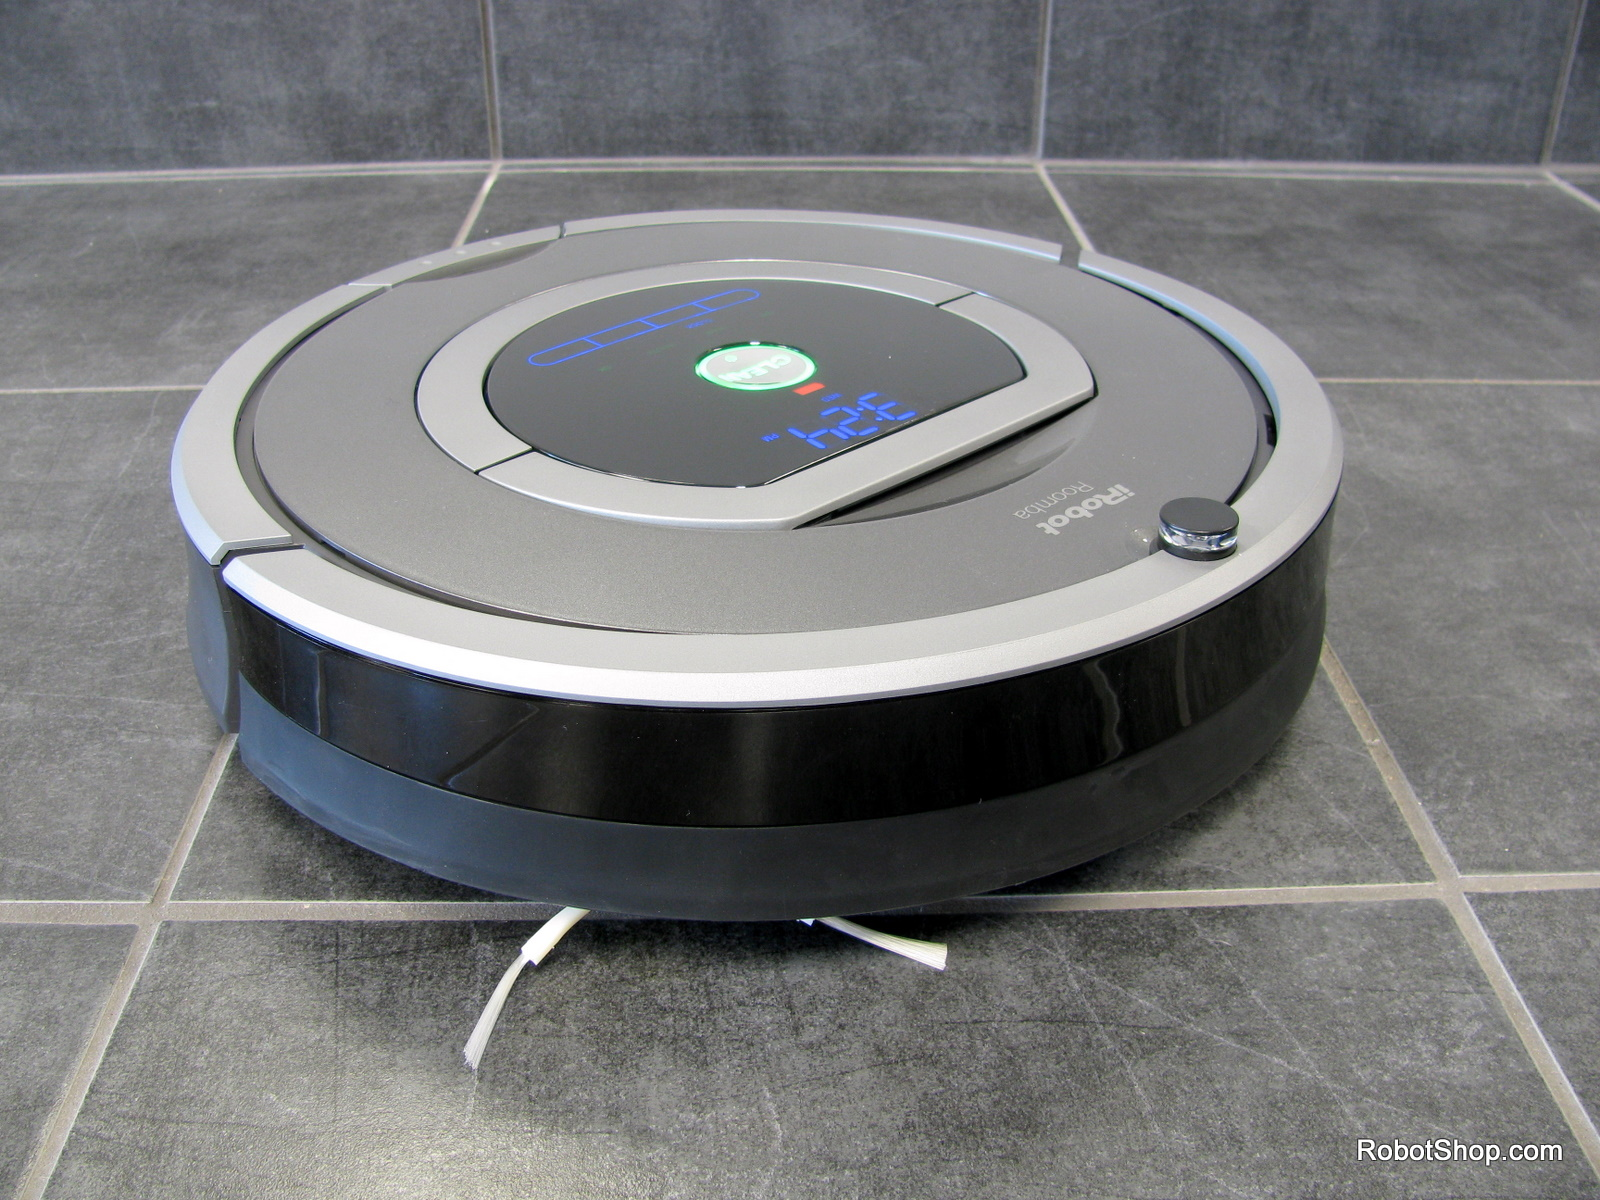
\includegraphics[width=67mm, keepaspectratio]{figures/iRobot_roomba_780.jpg}\hspace{1cm}
	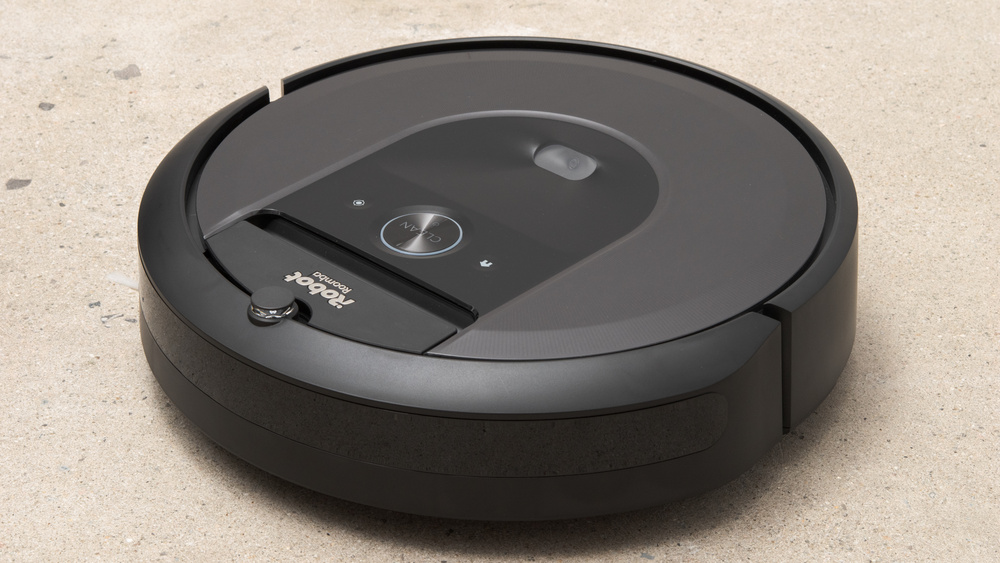
\includegraphics[width=67mm, keepaspectratio]{figures/iRobot_roomba_i7.jpg}\\\vspace{5mm}
	\caption{Robot vacuum cleaners iRobot Roomba 780 (left) and i7 (right), sources: \cite{roomba780}\cite{roombai7}}
	\label{fig:Roombas}
\end{figure}
\FloatBarrier
This example highlights the advantages of simultaneous localization and mapping (SLAM) in a household environment. SLAM technology is also transformative in industrial contexts. For instance, autonomous robots can transport heavy products across large warehouses. In such scenarios, a wall-to-wall navigation algorithm would be impractical, as it would likely fail to reach its destination before depleting its battery. Consequently, modern autonomous systems increasingly rely on SLAM algorithms to enable efficient and reliable navigation.

In industrial settings, autonomous robots are evolving beyond simple navigation tasks to handle more complex activities, such as moving and organizing inventory. As illustrated in Figure~\ref{fig:robots_in_warehouse}, robots equipped with manipulators can load packages onto mobile robots that transport items across warehouses. These combined systems of robotic arms and mobile platforms represent a new frontier for industrial automation, where robots can not only navigate large spaces but also carry out detailed, repetitive tasks that require precise movements and lifting capabilities. This level of automation has the potential to significantly increase operational efficiency, reduce human labor in hazardous or strenuous tasks, and streamline the logistics of large-scale storage and distribution.

\FloatBarrier
\begin{figure}[htbp]
	\centering
	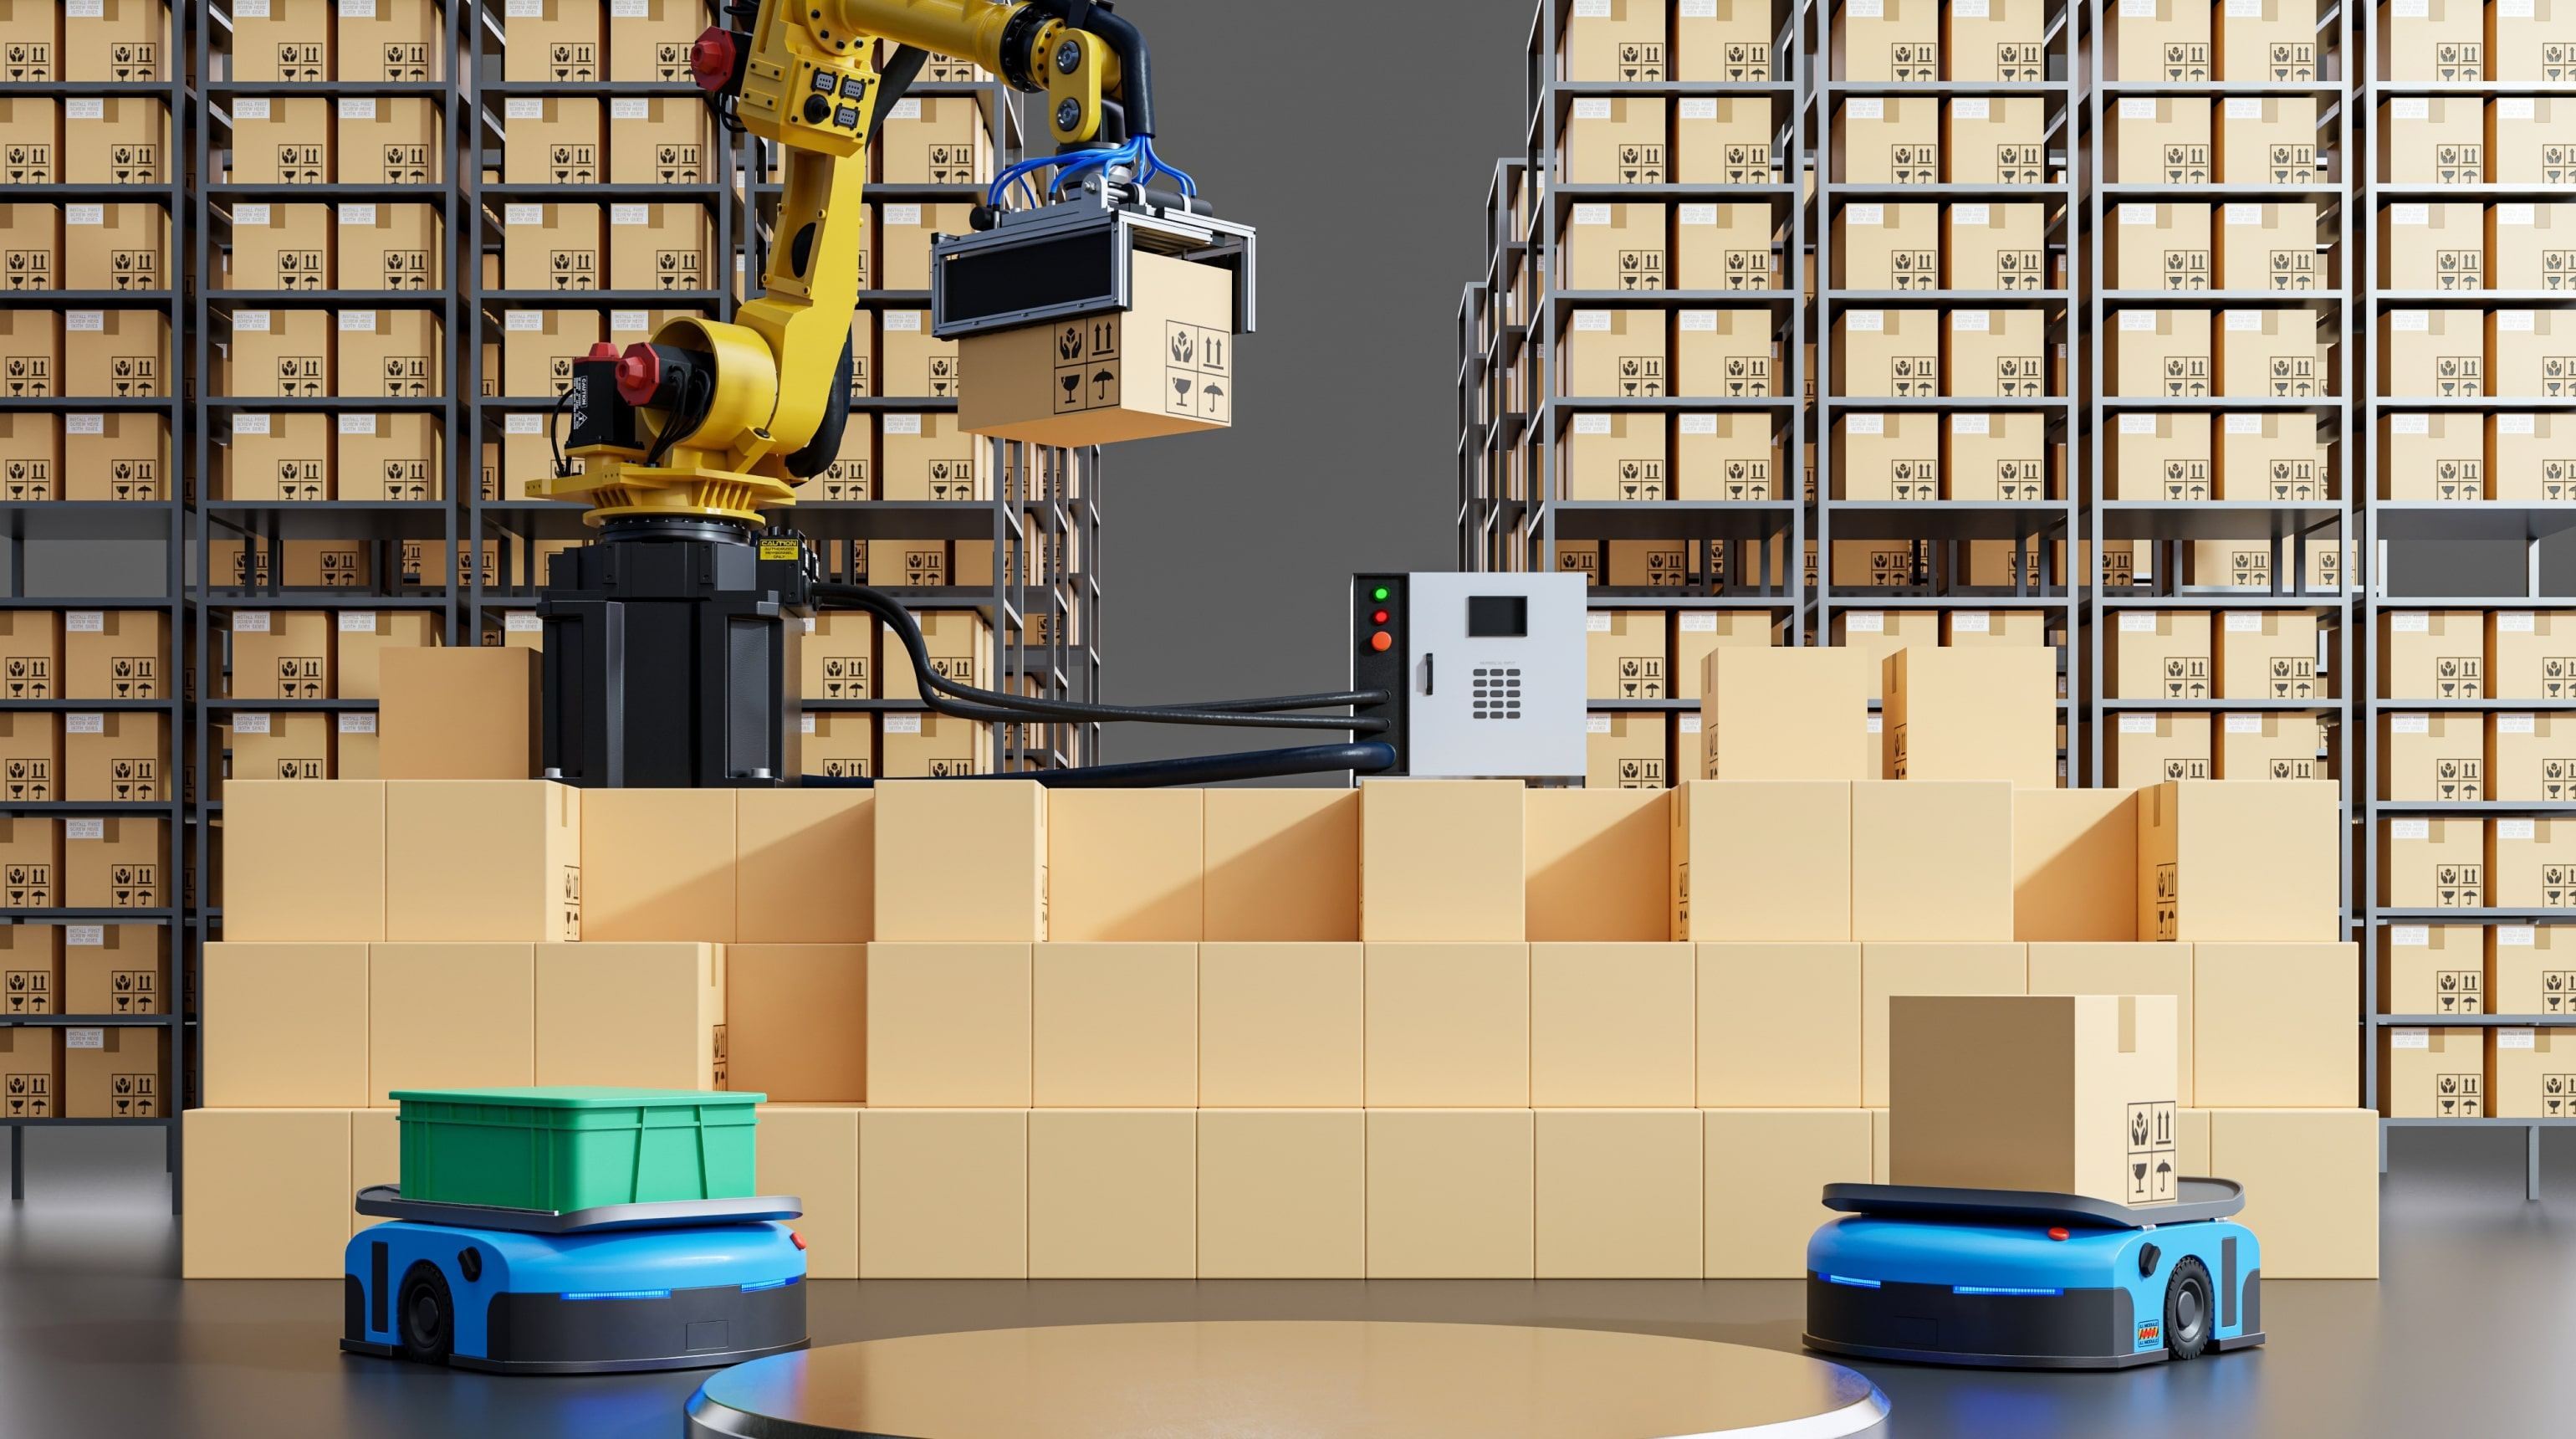
\includegraphics[width=150mm, keepaspectratio]{figures_jpg/warehouse_robots.jpg}
	\caption{Illustration of robots used in a warehouse, source:~\cite{robots_in_warehouse}}
	\label{fig:robots_in_warehouse}
\end{figure}
\FloatBarrier

In summary, SLAM plays an essential role in empowering mobile robots to understand and navigate their environments effectively, whether in homes or complex industrial settings.

Mobile robotics technology may one day extend to fully autonomous household assistants, as illustrated in Figure~\ref{fig:futuristic_house_cleaning_robot}. This concept envisions a future where robots with manipulators, or robotic "hands" perform routine household chores, such as loading the dishwasher or organizing items~\cite{physical_intelligence}. The development of such robots could revolutionize domestic life by reducing the time and effort spent on daily tasks, enabling greater convenience and flexibility for homeowners. As mobile robots become capable of not only navigating but also manipulating their environment, they have the potential to transform lifestyles, adding a new dimension to household automation and creating more time for people to engage in other activities.

\FloatBarrier
\begin{figure}[htbp]
	\centering
	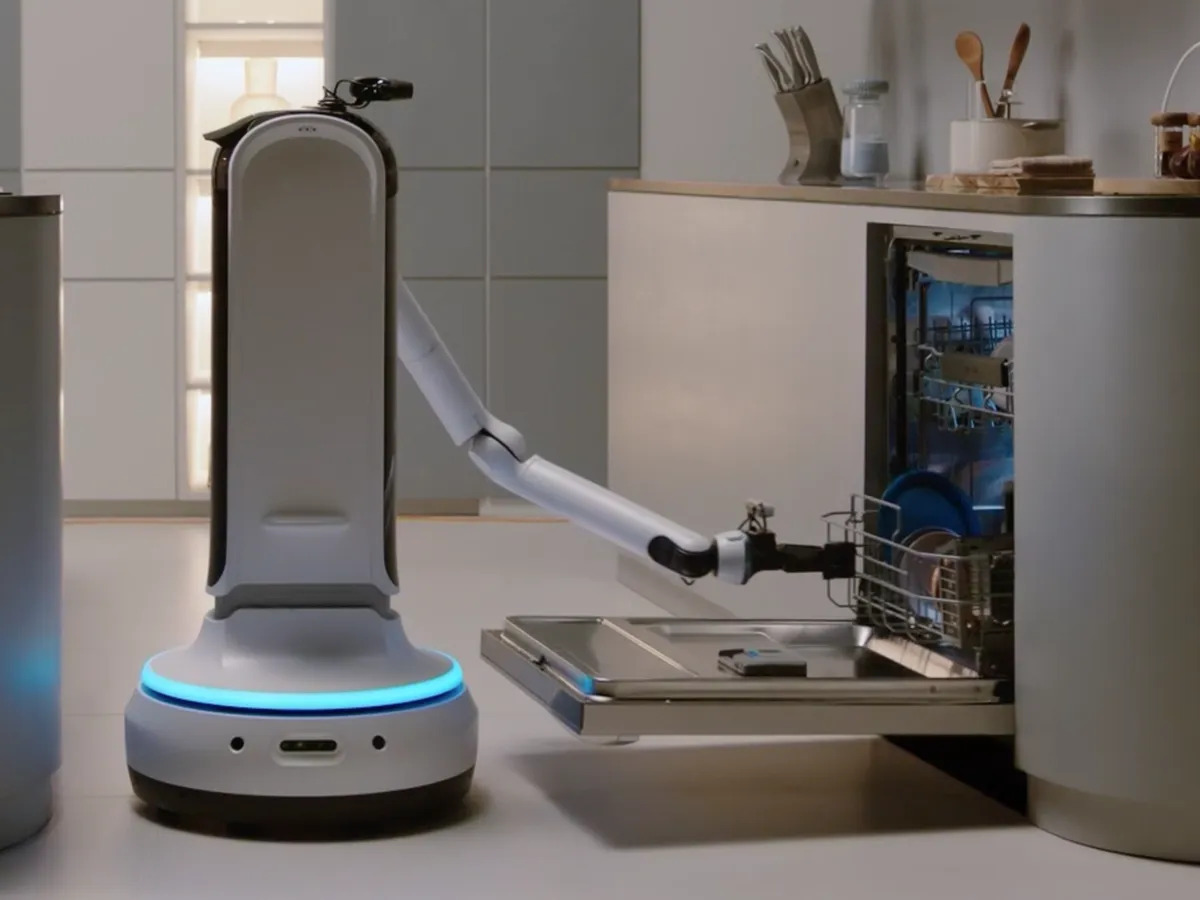
\includegraphics[width=150mm, keepaspectratio]{figures_jpg/samsung-bot-handy.jpg}
	\caption{A futuristic house cleaning robot, source:~\cite{futuristic_household_robot}}
	\label{fig:futuristic_house_cleaning_robot}
\end{figure}
\FloatBarrier

\section{Goal of the thesis}

The primary objective of this thesis is to advance the exploration and mapping capabilities of a (Roomba-like) mobile robot, enabling it to map new environments. The resulting map can then be reused by the robot itself or shared with other robots, supporting coordinated navigation and interaction in shared spaces.

The main focus of this work is to implement Visual SLAM (V-SLAM) using a stereo camera, as opposed to traditional SLAM methods that rely on LiDAR. Stereo cameras can capture detailed 3D maps or point clouds, enhancing the robot's spatial awareness.

In addition to these core objectives, two optional goals were pursued:
\begin{itemize}
\setlength\itemsep{0em}
    \item Person detection and tracking: Using the camera to identify and track people, allowing the robot to either follow or avoid them as needed.
    \item Photorealistic scene reconstruction: Generating high-quality, realistic representations of the environment for advanced visualization.
\end{itemize}

Through these goals, this thesis aims to enhance the utility, versatility, and adaptability of mobile robots in various environments by leveraging advanced V-SLAM techniques.


\section{Structure of the project and the thesis}

During the writing of my thesis, I have gained significant experience in many fields. First, I learned about the scientific background of mobile robotics, their odometry, localization, mapping, SLAM and photorealistic reconstruction, which I present in Chapter~\ref{background}. Then, I learned about the Robot Operating System, the robot used at Nokia Bell Labs, OAK-D cameras, neural reconstruction and different types of 3D mapping in Chapter~\ref{related_works}. After, I digged deeper in the capabilities of the OAK-D camera in Chapter~\ref{experiments_oak_d}, experimented with 3D mapping using RTAB-Map, nvblox and Isaac VSLAM in Chapter~\ref{experiments_3d_mapping}, and gained experience in photorealistic reconstruction with NeRFs and Gaussian Splatting in Chapter~\ref{nerf_gsplat}. Then, I implemented an end-to-end mapping and photorealistic reconstruction pipeline which is presented in Chapter~\ref{implementation}. I evaluated the reconstruction pipeline in Chapter~\ref{evaluation}, and I summarized the achievements of this thesis in Chapter~\ref{summary}.

\chapter{Background} \label{background}

In this chapter we are going to provide the scientific background of this thesis. The scientific and technological foundation of mobile robotics has evolved through research on various aspects of robot motion, environmental perception, mapping, and localization. This chapter provides an overview of the essential concepts underpinning autonomous navigation and scene reconstruction, which are crucial to the systems studied in this thesis. We explore mobile robotics, SLAM and its visual counterpart VSLAM, and the emerging fields of photorealistic reconstruction and visual-inertial odometry (VIO), all of which contribute to the ability of robots to navigate and interact with their environment effectively.

\section{Introduction to mobile robotics}

Mobile robotics focuses on the design, implementation, and control of autonomous robots that can navigate dynamic, unknown environments~\cite{probabilistic_robotics}. The field intersects with various sub-disciplines in engineering, computer science, and AI, aimed at developing intelligent systems capable of movement without human intervention. The integration of sensors, actuators, and computational algorithms in mobile robots has led to significant advancements, particularly in mapping and localization. Early contributions in the field laid the groundwork for more sophisticated robotic platforms, emphasizing the need for reliable localization, obstacle avoidance, and path planning~\cite{introduction_to_autonomous_mobile_robots}.

\section{Odometry in Mobile Robots}

Odometry is a fundamental concept in mobile robotics that deals with the estimation of a robot's position and orientation over time as it moves through an environment. This process typically involves measuring changes in position based on the motion of the robot’s wheels or other propulsion mechanisms. Odometry enables a robot to understand its incremental motion relative to a known starting point, providing essential information for navigation and positioning in environments where external localization sources (such as GPS) may be unavailable or unreliable.

\subsection{Basics of Odometry}

The traditional approach to odometry relies on wheel encoders, which measure wheel rotations to estimate the distance traveled. Using simple geometric relationships, the robot’s forward motion and changes in orientation can be calculated from these measurements. For differential drive robots, which have two wheels independently controlled on either side, changes in orientation are derived from the difference in distance traveled by each wheel. This is extended to omnidirectional platforms with multiple wheels or non-wheel-based odometry, depending on the robot's configuration~\cite{odometry_1996}.

Despite its simplicity and efficiency, wheel-based odometry is prone to cumulative error, particularly in environments where wheel slippage occurs due to uneven surfaces, loose materials, or sharp turns. These issues are more pronounced in outdoor or rugged terrains, where conventional odometry can yield highly inaccurate results without additional corrections~\cite{odometry_1996}.

\subsection{Error Accumulation and Correction in Odometry}

Odometry errors in mobile robots are typically classified as systematic and non-systematic errors. Systematic errors arise from mechanical imperfections, such as unequal wheel diameters or axle misalignments, which introduce biases in the measurements. These can often be minimized by careful calibration and parameter tuning. Non-systematic errors, on the other hand, result from unpredictable factors like wheel slip, bumps, and surface irregularities. These errors are challenging to mitigate solely with encoder data, as they vary with the environment and the robot’s movements~\cite{odometry_1996}.

To correct for these errors, sensor fusion techniques have been developed, integrating additional sensory data (e.g., inertial or visual data) to compensate for drift in wheel odometry. Sensor fusion algorithms, such as the Kalman Filter (KF)~\cite{kalman1960} and Extended Kalman Filter (EKF)~\cite{extended_kalman_filter}, have become standard tools in mobile robotics for filtering noise and improving the reliability of odometry-based position estimates. These probabilistic models enable the robot to maintain a statistically grounded estimate of its state by dynamically adjusting to sensor inputs and system uncertainties.

\subsection{Visual Odometry}

To overcome the limitations of traditional wheel odometry, researchers have developed Visual Odometry (VO), which uses cameras to estimate a robot’s position by tracking visual features across sequential frames. Visual odometry generally involves the following steps:

\begin{enumerate} 
    \item Feature Detection and Matching: Salient features, such as corners or edges, are detected in each camera frame, and corresponding features are matched in consecutive frames.
    \item Motion Estimation: From the matched features, the robot’s relative motion between frames is estimated using techniques like the Epipolar Geometry~\cite{epipolar_geometry} or Homography Transformation~\cite{homography_transformation} for planar surfaces.
    \item Optimization and Filtering: The motion estimates are then optimized and refined to minimize error and ensure continuity across frames~\cite{visual_odometry}.
\end{enumerate}

Two popular approaches to VO include monocular and stereo visual odometry:
\begin{itemize}
    \item Monocular Visual Odometry: This uses a single camera and estimates depth information through motion, based on the geometry between consecutive frames. Monocular VO is computationally efficient but lacks scale information, which can lead to scaling ambiguities~\cite{monocular_VO}.
    \item Stereo Visual Odometry: This employs two cameras, providing depth information directly from the disparity between the stereo images. Stereo VO is more accurate in terms of scale but requires higher computational resources and synchronization between cameras~\cite{stereo_VO}.
\end{itemize}

The robustness of VO depends on environmental factors such as lighting, texture, and dynamic objects. To address these challenges, modern VO systems often incorporate deep learning models to enhance feature extraction and improve motion estimates under challenging conditions~\cite{deepVO}.

\subsection{Visual-Inertial Odometry}

Visual-Inertial Odometry (VIO) is an extension of visual odometry that incorporates data from Inertial Measurement Units (IMUs)—sensors that measure accelerations and rotational velocities. By fusing visual and inertial data, VIO can provide a more robust estimate of the robot's trajectory, compensating for drift and error accumulation in environments with limited visual information or rapid motion.

Key components of VIO include:
\begin{enumerate}
    \item Preintegration of Inertial Data: IMU data is continuously integrated over time to estimate motion between frames, which is combined with visual data to provide a more stable trajectory.
    \item Non-linear Optimization: VIO systems often use non-linear optimization techniques to fuse the visual and inertial data, refining the robot’s pose estimates.
    \item Outlier Rejection: Given the inherent noise in IMU data and the potential for feature mismatches in visual odometry, outlier rejection techniques are essential to filter out erroneous data points~\cite{VIO}.
\end{enumerate}

Popular VIO frameworks, such as ROVIO (Robust Visual-Inertial Odometry)~\cite{robust_VIO} and VINS-Mono~\cite{vins_mono}, have demonstrated high accuracy and real-time performance in a wide range of robotic applications, from autonomous drones to ground vehicles. These systems rely on tight coupling of visual and inertial measurements, enabling robust odometry in diverse environments.

\subsection{Applications of Odometry in Mobile Robotics}

Odometry is a foundational component in a variety of mobile robotic applications, enabling robots to navigate complex environments, build maps, and interact with surroundings. Key applications include:
\begin{itemize}
    \item Autonomous Ground Vehicles: In autonomous ground vehicles, precise odometry is crucial for navigation and collision avoidance, particularly in indoor environments where GPS is unavailable. Odometry data aids in path planning and obstacle detection, ensuring safe and efficient navigation.
    \item Drone Navigation: Drones rely heavily on VIO due to their requirement for precise positioning during rapid maneuvers. VIO is effective in aerial applications, particularly indoors or in GPS-denied areas, enabling stable flight control and obstacle avoidance.
    \item Robotic Manipulation: In mobile manipulators, odometry is essential for coordinating the robot's position with its end effector movements, particularly in tasks requiring precision, such as assembly or inspection.
\end{itemize}

\section{Localization and mapping}

Localization and mapping are two essential, interconnected processes in mobile robotics that allow robots to navigate and understand their environment. Localization is the robot's ability to determine its position within a known map, while mapping is the process of creating a map of an unknown environment based on sensor data. These capabilities are crucial for autonomous navigation, enabling a robot to explore new spaces, recognize its location, and avoid obstacles.

Traditionally, localization and mapping were treated as separate problems, but the development of Simultaneous Localization and Mapping (SLAM)~\cite{slam} has integrated the two into a single framework, allowing a robot to localize itself while concurrently building a map of its surroundings. SLAM is now the dominant paradigm in mobile robotics, supporting diverse applications such as autonomous vehicles, drones, and industrial robots.

\subsection{Challanges in localization and mapping}

The localization and mapping processes involve several key challenges that must be addressed for effective operation in dynamic, real-world environments:
\begin{itemize}
    \item Data Association: Identifying and matching features in sensor data across different time steps is essential for accurate mapping. This is difficult in dynamic environments where objects may move or change appearance.
    \item Loop Closure: Detecting when a robot revisits a previously mapped location is critical for correcting drift in the map. Loop closure algorithms rely on feature recognition to identify previously seen areas, allowing the robot to refine its position and correct any accumulated error in its map~\cite{loop_closure}.
    \item Map Representation: The choice of map representation affects the accuracy and efficiency of both localization and mapping. Maps can be represented in various formats, including grid maps, feature-based maps, or topological maps, each with its advantages and limitations depending on the application~\cite{map_representations}.
    \item Computational Complexity: SLAM algorithms often require significant computational resources, especially in large-scale or complex environments. Balancing real-time performance with map accuracy and detail is a critical trade-off in SLAM development.
\end{itemize}

\subsection{Simultaneous Localization and Mapping}

Simultaneous Localization and Mapping (SLAM) is the process by which a robot builds a map of an unknown environment while simultaneously localizing itself within that map. SLAM algorithms generally consist of three primary components: sensor data processing, state estimation, and map optimization.

\begin{itemize}
    \item Sensor Data Processing: SLAM systems use data from sensors such as LiDARs, cameras, and inertial measurement units (IMUs) to obtain measurements of the robot’s surroundings. These sensors provide complementary data; for instance, LiDAR offers accurate distance measurements, while cameras capture visual features~\cite{slam_used_sensors}.
    \item State Estimation: SLAM algorithms estimate the robot's position and orientation by processing sensor measurements through probabilistic models like the Extended Kalman Filter (EKF)~\cite{extended_kalman_filter} or Particle Filters~\cite{particle_filter}. These models maintain an estimate of the robot’s state over time, adjusting as new sensor data is acquired.
    \item Map Optimization: Map optimization refines the robot’s position and the map representation by minimizing error through techniques like pose graph optimization. Loop closure detection and correction are integral parts of this process, enabling the system to handle long-term drift and maintain an accurate map~\cite{map_optimisation}.
\end{itemize}

SLAM can be categorized by the type of sensors used and the mathematical models employed, with popular variations including LiDAR-based SLAM, visual SLAM (VSLAM), and multi-sensor SLAM. Each of these approaches has unique advantages depending on the operating environment and computational constraints.

\subsection{LiDAR-Based SLAM}

LiDAR-based SLAM uses LiDAR sensors to measure distances by emitting laser beams and detecting their reflections~\cite{lidar}. This method creates precise maps of the environment, making it highly effective in indoor and outdoor settings with complex geometries. LiDAR-based SLAM algorithms, such as Hector SLAM~\cite{hector_slam} and Google’s Cartographer~\cite{google_cartographer}, leverage LiDAR's depth accuracy and robustness to ambient lighting changes, making them well-suited for autonomous ground vehicles, indoor robotics, and outdoor applications.

\subsection{Visual SLAM}

Visual SLAM (VSLAM) relies on cameras to capture visual features from the environment, using these features to localize the robot and create a map. VSLAM is particularly advantageous in environments where LiDAR may not be feasible or effective, such as environments containing dynamic objects, where a camera can be used to detect and exclude these objects. Key VSLAM techniques include:
\begin{itemize}
    \item Feature-based VSLAM: This approach detects and tracks visual features across consecutive frames. Algorithms like ORB-SLAM~\cite{orb_slam} and LSD-SLAM~\cite{lsd_slam} use these features to estimate motion and build a map.
    \item Direct VSLAM: Instead of relying on discrete feature points, direct VSLAM algorithms (e.g., DTAM~\cite{dtam}) use the intensity of all pixels in an image to estimate motion and map the environment. This method is often more robust in texture-less areas but requires greater computational resources.
    \item Deep Learning-Augmented VSLAM: Recent advancements in deep learning have introduced VSLAM algorithms that leverage convolutional neural networks (CNNs) to improve feature extraction, depth estimation, and dynamic scene understanding. These enhancements are particularly valuable in challenging conditions where traditional feature-based methods struggle~\cite{deep_learning_vslam}.
\end{itemize}

\subsection{Multi-sensor SLAM}

Multi-sensor SLAM integrates data from various sensors (LiDAR, cameras, IMUs) to overcome the limitations of single-sensor SLAM systems. Multi-sensor fusion is particularly valuable in environments where no single sensor can provide reliable data alone. For example, IMUs can compensate for rapid movements that cause motion blur in cameras, while LiDAR provides accurate distance measurements in environments where visual data might be unreliable due to lighting conditions.

Multi-sensor SLAM algorithms typically use Kalman filters~\cite{kalman1960}, Particle filters~\cite{particle_filter}, or factor graphs~\cite{factor_graph} to fuse data and estimate the robot’s state with increased robustness. Approaches like QN-SAM-LIVO~\cite{qn_sam_livo} have successfully integrated LiDAR, visual and inertial data to achieve real-time, high-accuracy localization and mapping in diverse environments.

\subsection{Applications of Localization and Mapping in Robotics}

The ability to localize and map autonomously has numerous applications in modern robotics, including:
\begin{itemize}
    \item Autonomous Vehicles: Self-driving cars require highly accurate maps of urban environments to navigate safely. LiDAR and camera-based SLAM systems provide the localization and situational awareness necessary for tasks like lane-following, obstacle detection, and traffic sign recognition~\cite{slam_for_autonomous_driving}.
    \item Drones and Aerial Robotics: For drones, localization and mapping are critical for stable flight control and collision avoidance. VSLAM and VIO techniques are widely used to enable drones to navigate in GPS-denied environments, such as indoors or densely forested areas~\cite{d2slam}.
    \item Service Robots: Indoor robots used in warehouses or hospitals rely on SLAM to navigate and interact with objects, providing services such as delivery, cleaning, and inspection. Grid-based or feature-based SLAM methods are commonly used in these applications~\cite{slam_for_service_robots}.
\end{itemize}

\section{Photorealistic reconstruction}

Photorealistic reconstruction refers to the process of creating highly detailed, lifelike 3D models of real-world environments, objects, or scenes. This is achieved by capturing fine visual details, textures, lighting, and spatial information that make the reconstruction indistinguishable from real life. The primary objective of photorealistic reconstruction is to generate virtual representations that maintain the visual fidelity and geometric accuracy required for applications like virtual reality (VR), augmented reality (AR), and, increasingly, mobile robotics. For robotics, these reconstructions are crucial for enhancing perception, improving decision-making in navigation, and enabling robots to interact effectively with their surroundings.

\subsection{Overview of 3D reconstruction}

3D reconstruction techniques in computer vision and graphics have evolved from simple geometric models to highly sophisticated, texture-rich models capable of photorealistic fidelity. The primary steps involved in 3D reconstruction include~\cite{3d_reconstruction_steps}:
\begin{enumerate}
    \item Data Acquisition: Data is captured using sensors like RGB cameras, depth sensors, LiDAR, or stereo cameras. Each sensor type contributes different information, such as color, depth, or surface structure, which together form the basis of a 3D model.
    \item Point Cloud Generation: A point cloud is generated from the sensor data, representing the 3D coordinates of points on object surfaces or environmental features. Point clouds provide the fundamental spatial structure of the scene.
    \item Surface Reconstruction: From the point cloud, surfaces are generated through techniques like triangulation, creating a mesh that connects these points into a continuous model. This process is refined to ensure smoothness, accuracy, and alignment with real-world geometry.
    \item Texturing and Shading: To achieve photorealism, textures and lighting effects are applied to the mesh. Texturing involves projecting captured images or textures onto the model surface, while shading uses lighting information to enhance realism, simulating shadow and reflection effects.
\end{enumerate}

Early 3D reconstruction methods relied heavily on explicit geometric modeling, but recent advancements in deep learning have introduced data-driven techniques that can capture finer details, handle occlusions, and generate more realistic scenes with less manual intervention. Neural networks have enabled significant breakthroughs in photorealistic reconstruction by directly learning 3D representations from visual data.

In robotics, photorealistic reconstruction is invaluable for creating detailed 3D maps of environments, especially in applications where accurate visual information is essential for effective robot-environment interactions. The following techniques are prominent in photorealistic reconstruction for robotics, each providing unique benefits depending on the required level of detail, processing power, and environmental complexity.

\subsection{Neural Radiance Fields}

Neural Radiance Fields (NeRFs) are a breakthrough in photorealistic reconstruction that use neural networks to generate high-fidelity 3D representations of scenes from 2D images. NeRFs work by modeling the color and density of rays passing through a 3D space, which allows the model to synthesize novel views from arbitrary angles. The core of NeRF lies in its ability to represent complex scenes using a volumetric neural network, which estimates the appearance of each pixel by blending colors and densities along rays cast through a scene~\cite{nerf}.

NeRF uses a set of 2D images from multiple viewpoints as input. By training a neural network to predict the color and opacity along each viewing ray, NeRF learns a volumetric representation of the scene. This process enables it to reconstruct realistic lighting and textures that would be challenging to achieve with traditional 3D models.

NeRFs are highly beneficial in robotics for generating realistic and immersive 3D maps of an environment. This is particularly useful for simulated environments, where robots can be trained in photorealistic virtual spaces before being deployed in the real world. In scenarios like object manipulation or navigation in visually complex environments, NeRF-based reconstructions allow robots to make better-informed decisions by leveraging visual cues similar to those in real-world scenes.

Despite its photorealistic quality, NeRF is computationally intensive and requires significant GPU resources for training, making it challenging to implement in real-time applications. However, recent work has focused on optimizing NeRF for faster inference and deployment on mobile robotic platforms~\cite{nerfhub}.

\subsection{Gaussian Splatting}

Gaussian Splatting is another novel approach to photorealistic reconstruction that models 3D scenes using Gaussian functions rather than point clouds or meshes. Each Gaussian represents a small, localized portion of the scene, allowing Gaussian Splatting to generate smooth and continuous reconstructions with high efficiency~\cite{3DGS}. Gaussian Splatting uses fewer memory resources compared to dense point clouds or neural networks, making it highly suitable for real-time applications in robotics.

In Gaussian Splatting, a 3D scene is approximated using Gaussian functions placed at points of interest in the environment. These Gaussians are blended to create a continuous surface, and their parameters are optimized to achieve high visual fidelity. By adjusting Gaussian parameters like mean, covariance, and intensity, Gaussian Splatting can replicate complex surfaces and textures in real-time.

Gaussian Splatting is effective for large-scale mapping and outdoor applications, where computational efficiency and memory usage are critical. Drones, for example, can use Gaussian Splatting to rapidly construct and update 3D models of expansive outdoor environments. Gaussian Splatting’s efficient memory usage allows it to perform real-time updates, making it ideal for navigation, exploration, and environmental monitoring in mobile robots~\cite{active_splat}.

While Gaussian Splatting is efficient, it may not achieve the same level of photorealistic quality as NeRFs, especially in capturing fine texture details. However, for many robotic applications, its speed and memory efficiency make it a practical alternative. Recent studies show that it is possible to convert NeRFs' outputs to Gausssian Splattings' outputs and vice versa, making the computational requirements lower than training both from scratch~\cite{nerf_gsplat_convert}.

\subsection{Applications of Photorealistic Reconstruction in Robotics}

Photorealistic reconstruction techniques are transforming the capabilities of mobile robotics by enhancing perception, enabling realistic simulation environments, and improving interactions with objects and scenes. Key applications of photorealistic reconstruction in robotics include:

\begin{itemize}
    \item Navigation and Path Planning: High-fidelity maps with realistic textures and lighting provide richer information for autonomous navigation. Robots can use photorealistic reconstructions to identify landmarks, avoid obstacles, and follow paths that are visually consistent with the real world~\cite{active_splat}.
    \item Simulation and Training: Simulations that incorporate photorealistic reconstructions allow robots to be trained in virtual environments that closely mirror real-world conditions. This is particularly useful in reinforcement learning, where robots can learn from interactions with highly realistic scenes, reducing the gap between simulated and real-world performance~\cite{reinforcement_learning_robot}.
    \item Object Recognition and Manipulation: Photorealistic 3D models of objects improve a robot's ability to recognize and interact with complex shapes. Robots can use NeRFs or Gaussian Splatting reconstructions to identify objects based on visual and spatial cues, facilitating tasks like grasping, sorting, and assembly.
    \item Environmental Monitoring and Mapping: For applications like environmental monitoring, search and rescue, or archaeological documentation, photorealistic reconstructions capture important details, preserving visual information for analysis. Drones equipped with cameras can fly over large areas and create detailed maps, allowing scientists or first responders to assess environments in high fidelity~\cite{drone_3d_reconstruction}.
    \item Human-Robot Interaction: Robots used in collaborative settings, such as service robots or healthcare assistants, benefit from photorealistic models that help them understand and interpret human environments. For instance, a service robot in a home can navigate more effectively if it can distinguish furniture and objects with high accuracy. Recent studies show that it can even be used in healthcare where it is possible to create 3D reconstruction of slowly healing wounds~\cite{3d_reconstruction_wounds}.
\end{itemize}

\chapter{Applied technologies} \label{related_works}

This chapter provides a comprehensive overview of the key technologies utilized in this thesis, detailing their capabilities, applications, and relevance to the project. Each section explores a specific technology or framework that was instrumental in the development and implementation of the robotic system.

The technologies discussed include the Robot Operating System 2 (ROS2), which serves as the foundation for communication and coordination within the robotic system, and the Turtlebot4, the mobile robotic platform used for experimentation. Additionally, the chapter delves into the hardware components integrated into the platform, such as the Raspberry Pi 4, RPLIDAR-A1, and OAK-D cameras, highlighting their roles in sensor fusion and environmental perception.

Furthermore, the chapter introduces software frameworks like the Spectacular AI SDK, which supports advanced visual-inertial tracking and mapping, and NVIDIA’s nvblox, a GPU-accelerated mapping library for real-time 3D reconstruction. It also touches upon state-of-the-art methodologies like Gaussian splatting and RTAB-Map, which enable advanced 3D visualization and real-time SLAM, respectively.

This chapter serves as both a technical foundation and a reference for the methods and tools that underpin the contributions of this thesis.

\section{Robot Operating System}

The ROS2 \cite{ROS2} (Robot Operating System 2) is not an operating system despite its name; it is a comprehensive framework for building robotic systems. This framework facilitates the development, deployment, and management of complex robotic applications by providing a collection of tools, libraries, and conventions designed to simplify the process.

At the core of ROS2 are executable units known as \textit{Nodes}. Each node is responsible for a specific task, such as sensor data processing, actuation, or decision-making. Nodes communicate with each other using a publish-subscribe messaging system, where messages are exchanged over channels called \textit{Topics}. This decoupled communication model allows for modular and flexible system design, enabling developers to easily add, remove, or modify nodes without affecting the entire system.

In addition to topics, ROS2 supports \textit{Services} and \textit{Actions}. Services provide a synchronous client-server communication model where a client sends a request to a server and waits for a response. This is useful for operations that require an immediate result, such as querying the state of a sensor or initiating a simple action.

Actions, on the other hand, are designed for long-running tasks. They allow a client to send a goal to an action server, which then executes the task and provides periodic feedback on its progress. This feedback mechanism is particularly useful for navigation tasks, where continuous updates on the robot's position, orientation, and status are essential. An action comprises a client node, a server node, a goal, and result services, along with a feedback topic, making it suitable for tasks that require continuous monitoring and dynamic adjustments.

One of the most compelling advantages of ROS2 is its language-agnostic design. Nodes can be written in multiple programming languages, primarily C++ and Python, and they can interoperate seamlessly. This interoperability is ensured by the strict message type definitions for topics, services, and actions, which remain consistent across different languages. This feature allows developers to leverage the strengths of each language; for instance, C++ for performance-critical tasks and Python for rapid prototyping and development.

In our research, we leverage ROS2 to integrate and manage the various components of our robotic system, including sensor integration and real-time mapping. The modularity and flexibility provided by ROS2 enable us to experiment with different approaches and quickly adapt to new requirements or challenges that arise during the development process.

\section{Turtlebot4}
At Nokia, we worked on a Turtlebot4\footnote{\url{https://clearpathrobotics.com/turtlebot-4/}} which consists of an iRobot Create3 base\footnote{\url{https://edu.irobot.com/what-we-offer/create3}}, a Raspberry Pi 4 host computer, and a companion laptop attached to it. Create3 is a robot vacuum cleaner's base made for educational use. It contains the differential drive, the IR proximity sensors in the front and the docking station for charging. All in all, it can be used to build more complex mobile robots.
A stereo camera and a rotating horizontal LiDAR are connected to the host computer via USB and the robot is connected to the notebook via Gigabit Ethernet so they can communicate over ROS topics. A diagram of the mentioned structure can be examined on Figure \ref{fig:mobile_robot_architecture}. The Turtlebot4 comes in two editions depending on equipment, we used the standard version. An image of the two editions of the robot can be seen on Figure \ref{fig:turtlebot4}.

\begin{figure}[htbp]
    \centering
    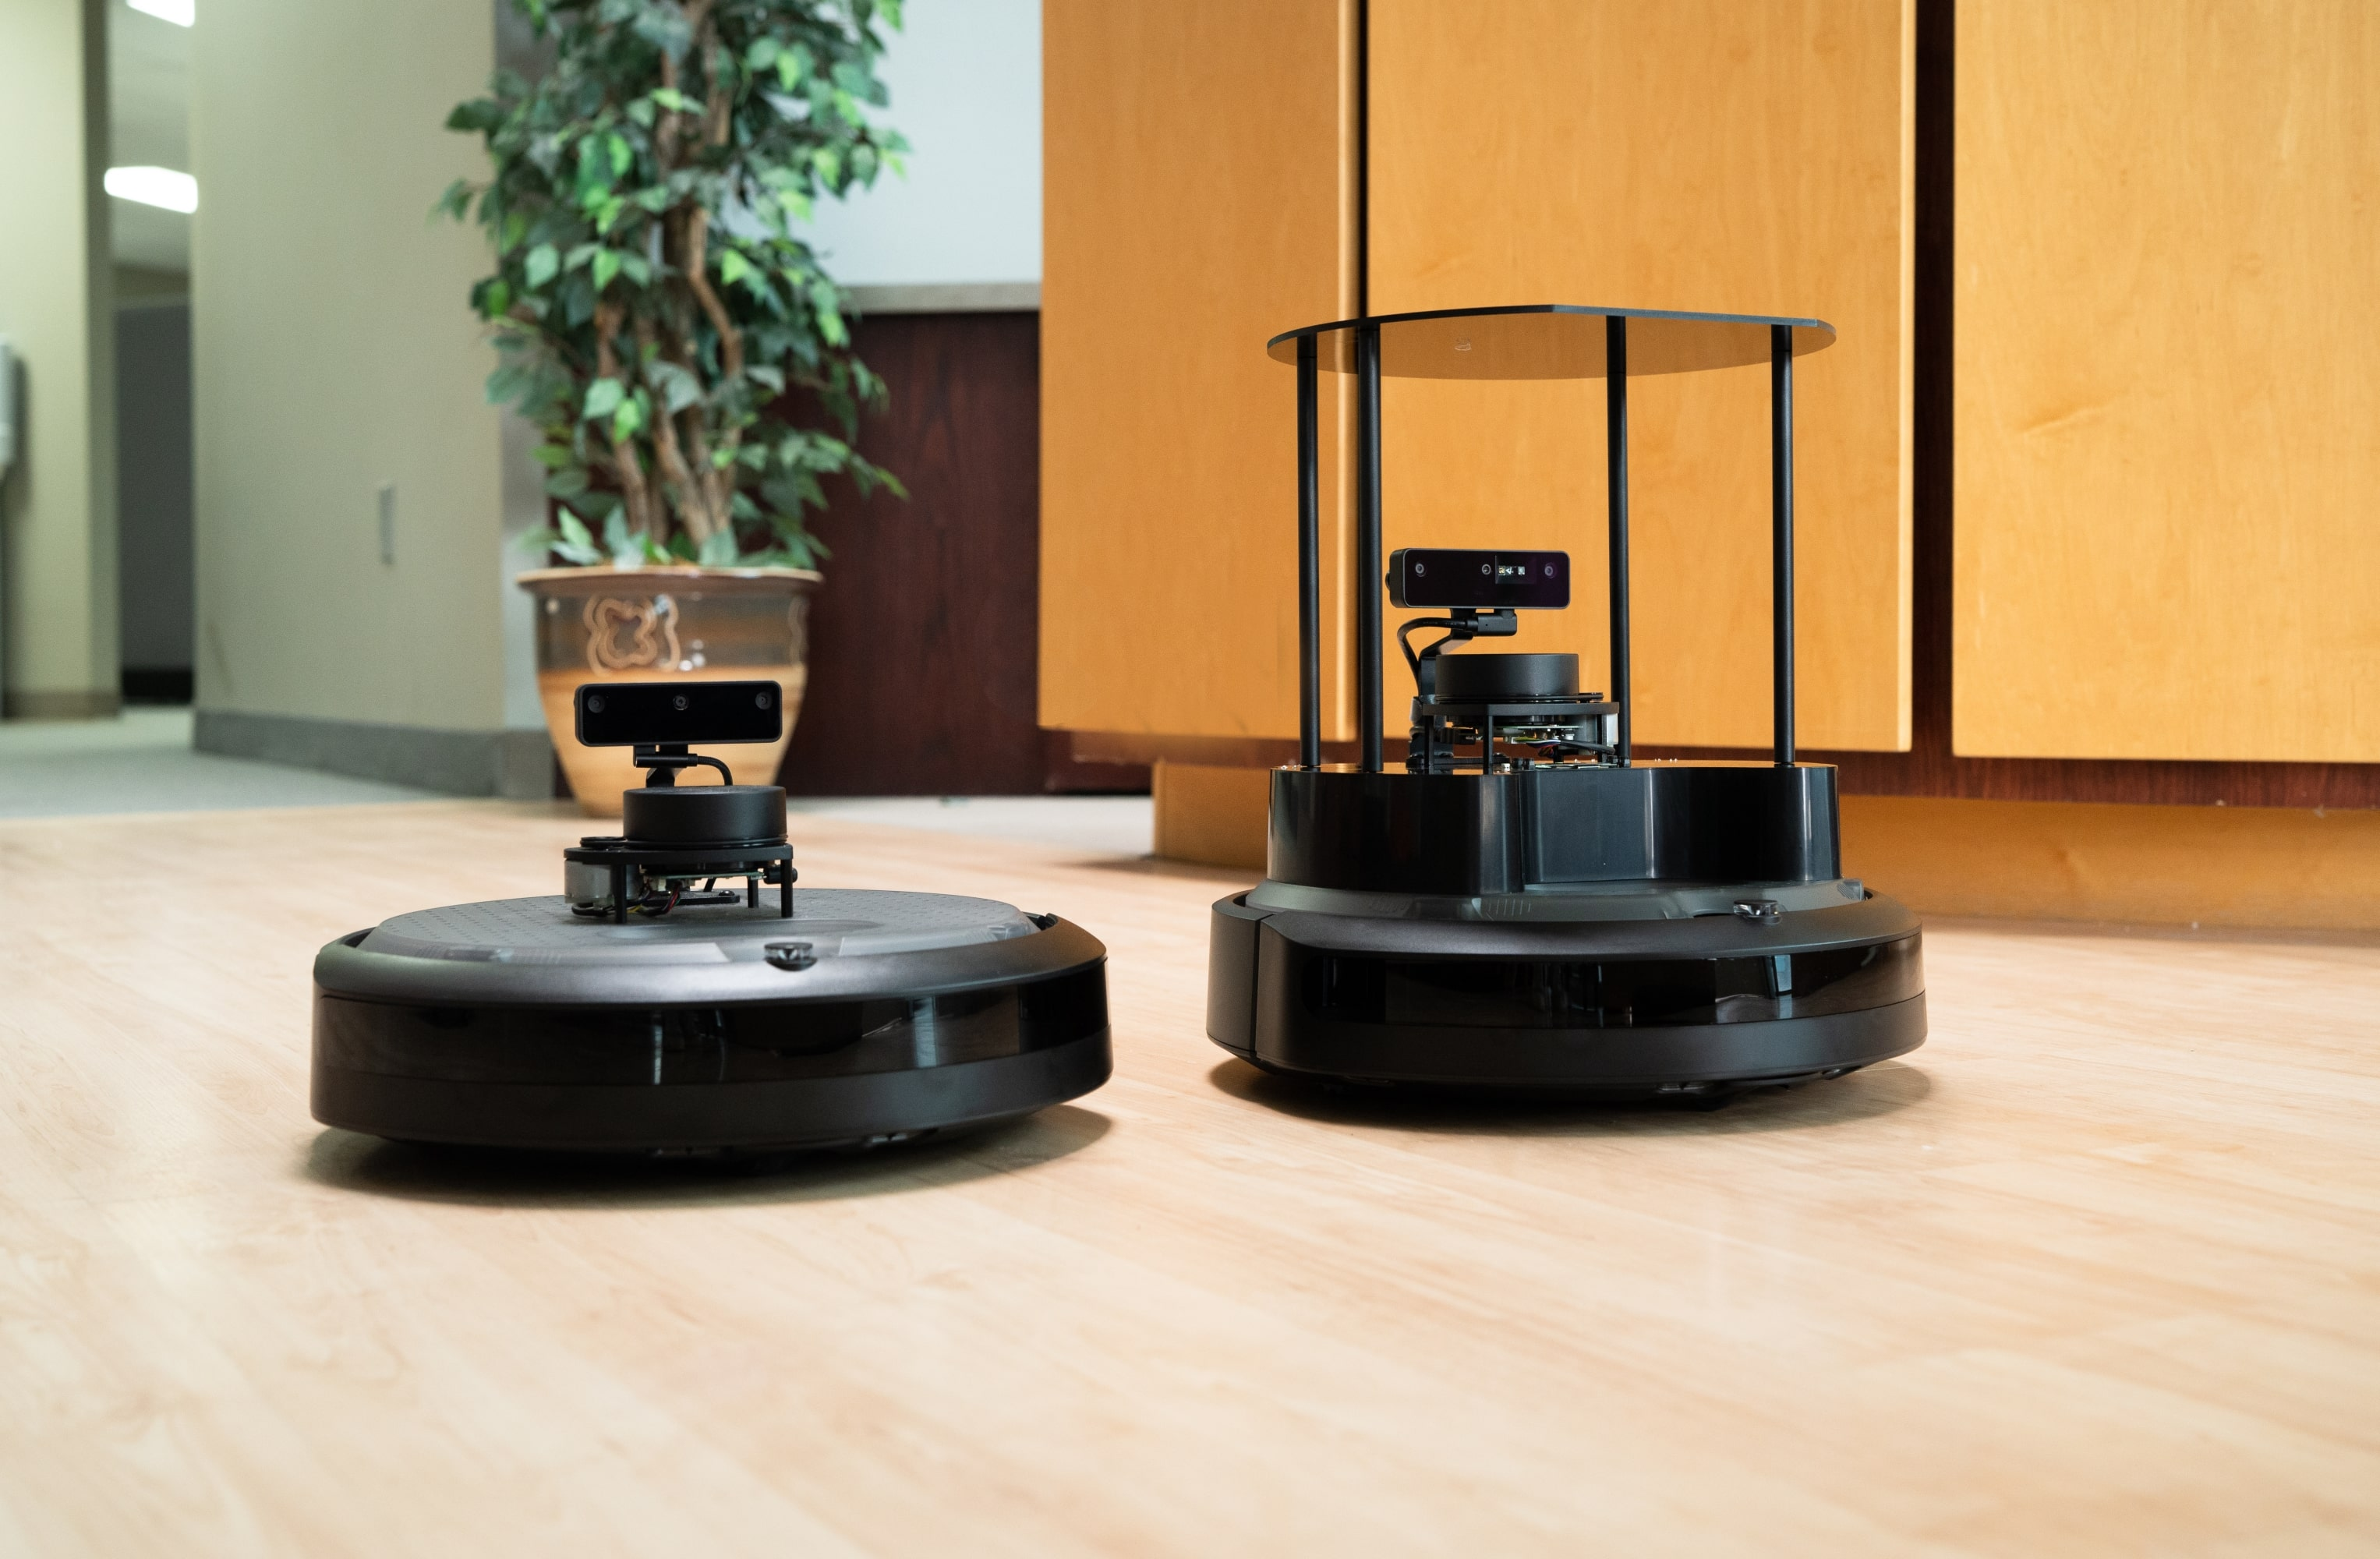
\includegraphics[width=150mm, keepaspectratio]{figures/TurtleBot4.jpg}
    \caption{Turtlebot4 Lite (left) and Turtlebot4, source:\cite{Turtlebot4Pic}}
    \label{fig:turtlebot4}
\end{figure}

\begin{figure}[htbp]
    \centering
    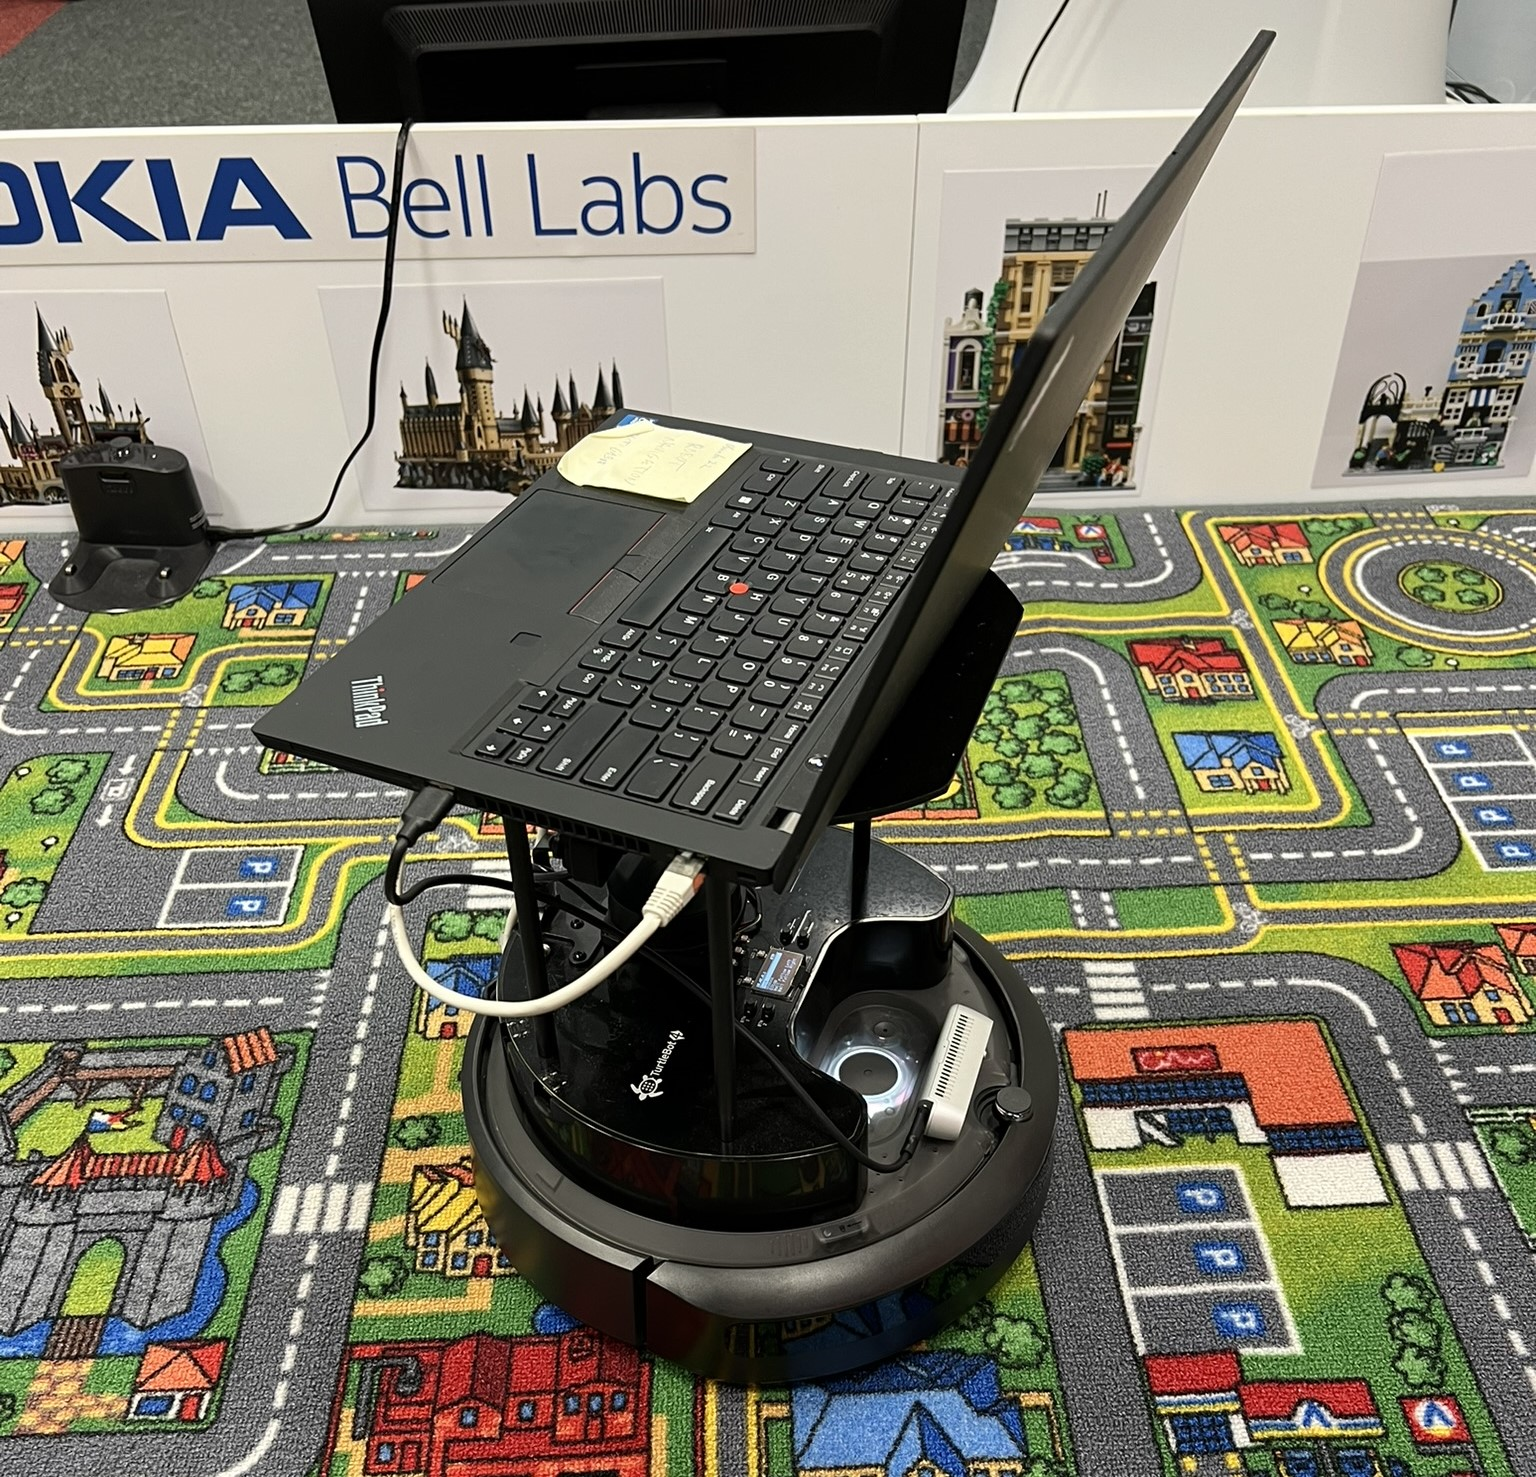
\includegraphics[width=150mm, keepaspectratio]{figures/turtlebot4_nokia.JPEG}
    \caption{Turtlebot4 at Nokia Bell Labs}
    \label{fig:turtlebot4_nokia}
\end{figure}




The host computer of the robot, a Raspberry Pi 4\footnote{\url{https://www.raspberrypi.com/products/raspberry-pi-4-model-b/}} is a mini PC which can be used in various applications:
at home as a desktop PC,
as a NAS (Network-Attached Storage),
as a media server,
in complex embedded systems,
in mobile robots, just to name only a few examples.
The Raspberry Pi 4 is equipped with a quad core ARM v8 Cortex-A72\footnote{\url{https://www.arm.com/products/silicon-ip-cpu/cortex-a/cortex-a72}} 64-bit SoC, Gigabit ethernet, 2 micro-HDMI ports which support resolution up to 4K, an USB-C power input and 2, 4 or 8 GB of RAM (it can be chosen by our needs or budget). In the Turtlebot4 the Raspberry Pi is used to run ROS2.


The Turtlebot4 is equipped with an RPLIDAR-A1\footnote{\url{https://www.slamtec.ai/product/slamtec-rplidar-a1/}} by Slamtech. It is a 2D LIDAR which can scan its surroundings up to 12 meters in 360°. Its maximum resolution is 1° with a maximum sampling frequency of 1\,Hz.
The sensor is plug-and-play, it has a USB interface, open-source SDK and ROS2 integration. It goes without saying, but it is worth noting that it meets the Class 1 laser safety standard and is completely safe for human eyes~\cite{LaserSafety}.

%\subsection{OAK-D Pro}
The Turtlebot 4 Standard also comes with an OAK-D Pro stereo camera as seen on Figure~\ref{fig:oak_d_pro_nokia}. OAK\footnote{\url{https://shop.luxonis.com/collections/oak-cameras-1}} is a robotic vision camera series made by Luxonis\footnote{\url{https://www.luxonis.com/}}, which sensors are pre-calibrated during manufacturing. Additionally, I got another OAK-D model from Nokia to test my implementations at home during the writing of my thesis.

The specifications of the OAK-D and OAK-D Pro:
\begin{table}[h!]
\centering
\begin{tabular}{|>{\raggedright\arraybackslash}p{0.45\linewidth}|>{\raggedright\arraybackslash}p{0.45\linewidth}|}
\hline
\textbf{OAK-D} & \textbf{OAK-D Pro} \\
\hline
\begin{itemize}
    \setlength\itemsep{0em}
    \item it has an IMX378 color camera,
    \item a pair of OV9282 as the stereo cameras (grayscale),
    \item an integrated 9-axis IMU,
    \item a VPU that can run neural network models.
\end{itemize} &
\begin{itemize}
    \setlength\itemsep{0em}
    \item it has an IMX378 Auto-Focus color camera,
    \item a pair of OV9282 as stereo cameras (greyscale),
    \item it contains the VPU and the IMU as well,
    \item it supports active stereo,
    \item it has IR illumination for night vision.
\end{itemize} \\
\hline
\end{tabular}
\caption{Specifications of OAK-D and OAK-D Pro}
\end{table}


\begin{figure}[htbp]
    \centering
    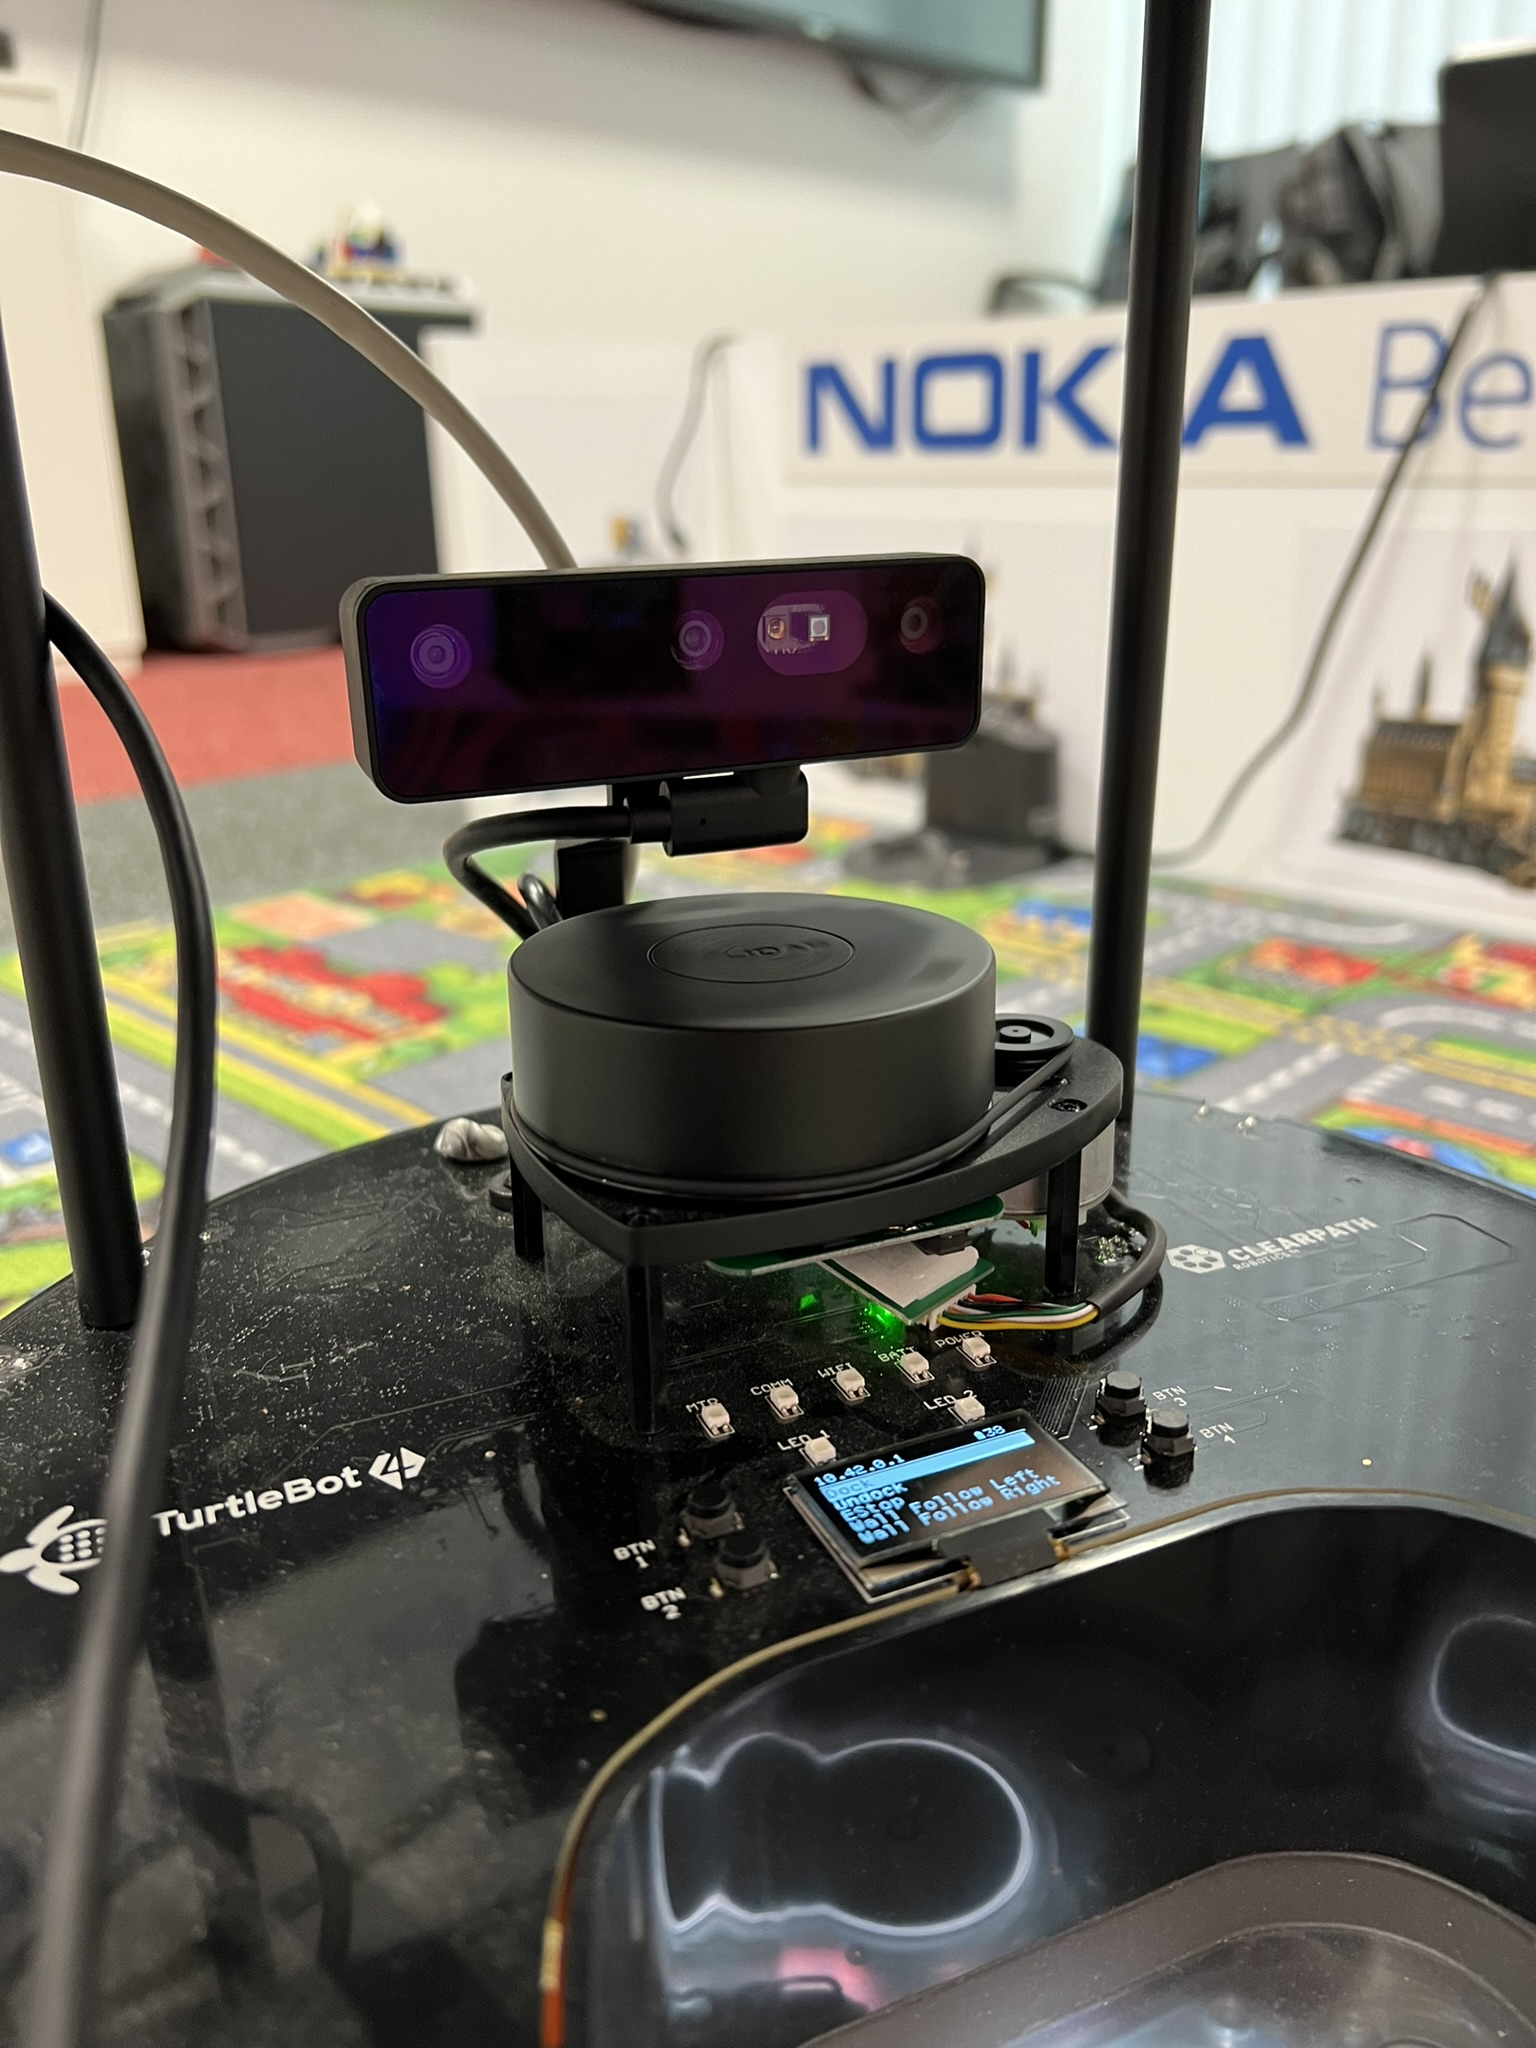
\includegraphics[width=100mm, keepaspectratio]{figures/oak_d_pro_nokia.JPEG}
    \caption{OAK-D Pro on a Turtlebot4 at Nokia Bell Labs}
    \label{fig:oak_d_pro_nokia}
\end{figure}

There are passive and active stereo cameras.
Passive stereo means the disparity between two cameras to calculate the distances between the camera and the scene points. By back-projecting a depth map into the scene, we can create a 3D point cloud of our surroundings. This method works best in environments with diverse textured surfaces because the stereo matching algorithm can only calculate the disparity values if the two cameras can see and identify corresponding points on their images. In case we point the camera to a textureless surface (for example a clean white wall) it will not be able to calculate the distances due to the lack of matching points. 
Active stereo cameras project an infrared light pattern into the scene, so they are able to find matching points even on textureless surfaces. The difference between the two methods can be observed on Figure~\ref{fig:active-passive-stereo}.

\begin{figure}[htbp]
    \centering
    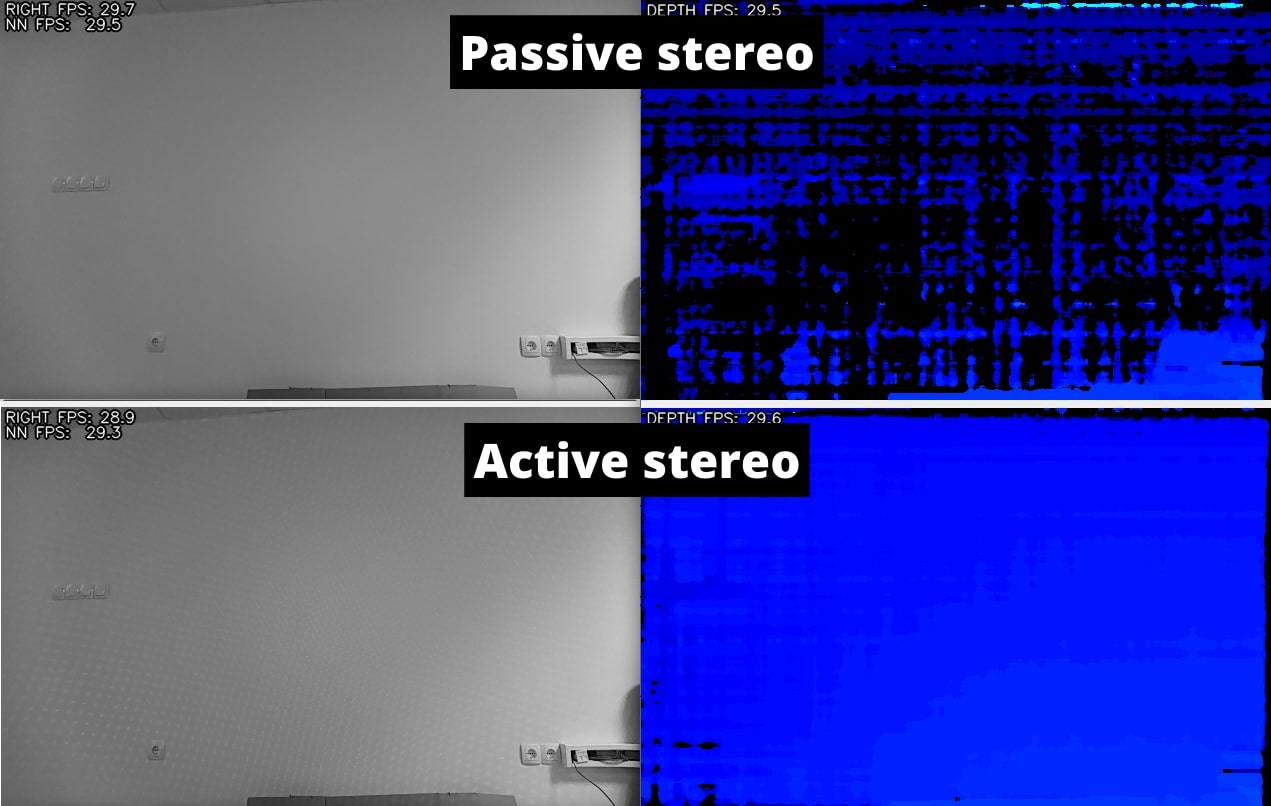
\includegraphics[width=100mm, keepaspectratio]{figures_jpg/active-vs-passive-stereo.jpg}
    \caption{Passive vs active stereo feature matching, source:\cite{ActivePassiveStereo}}
    \label{fig:active-passive-stereo}
\end{figure}

\begin{figure}[htbp]
    \centering
    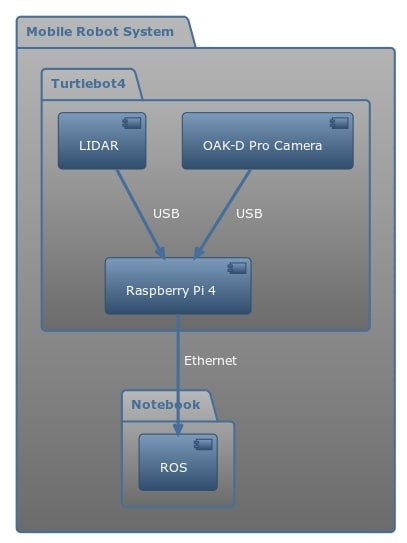
\includegraphics[width=50mm, keepaspectratio]{figures_jpg/turtlebot4_architecture.jpg}
    \caption{Architectural diagram of the mobile robot system at Nokia Bell Labs}
    \label{fig:mobile_robot_architecture}
\end{figure}

\FloatBarrier
\section{Spectacular AI SDK}

Spectacular AI\footnote{\url{https://www.spectacularai.com/}} is a Finnish company specialized on spatial visual-inertial motion tracking and 3D mapping. They provide an SDK\footnote{\url{https://github.com/SpectacularAI/sdk}} that can be used for various applications:
% Ensure no floats before the list
\FloatBarrier
\begin{itemize}
\setlength\itemsep{0em}
    \item pose tracking using camera and IMU fusion,
    \item point cloud mapping,
    \item 3D visualization of the agent trajectory
    \item AR mapping with meshes or point clouds,
    \item mapping with ROS2 visualization.
\end{itemize}
% Ensure no floats within the list
\FloatBarrier
The primary objective of the SDK is to assist in performing SLAM using an OAK camera. It supports working with ROS through some basic ROS nodes and bridges. The SDK's main strength is the usage of the IMU and VPU in the OAK camera.


\section{RTAB-Map}

RTAB-Map\footnote{\url{https://introlab.github.io/rtabmap/}} (Real-Time Appearance-Based Mapping~\cite{RTAB_Map_docs}) is a graph-based SLAM approach designed for long-term and large-scale mapping in real-time. It is widely used in robotics applications due to its capability to create detailed and accurate maps while efficiently managing computational resources. The mapping process can be seen on Figure~\ref{fig:rtabmap_applied_techs}.

\begin{figure}[htbp]
    \centering
    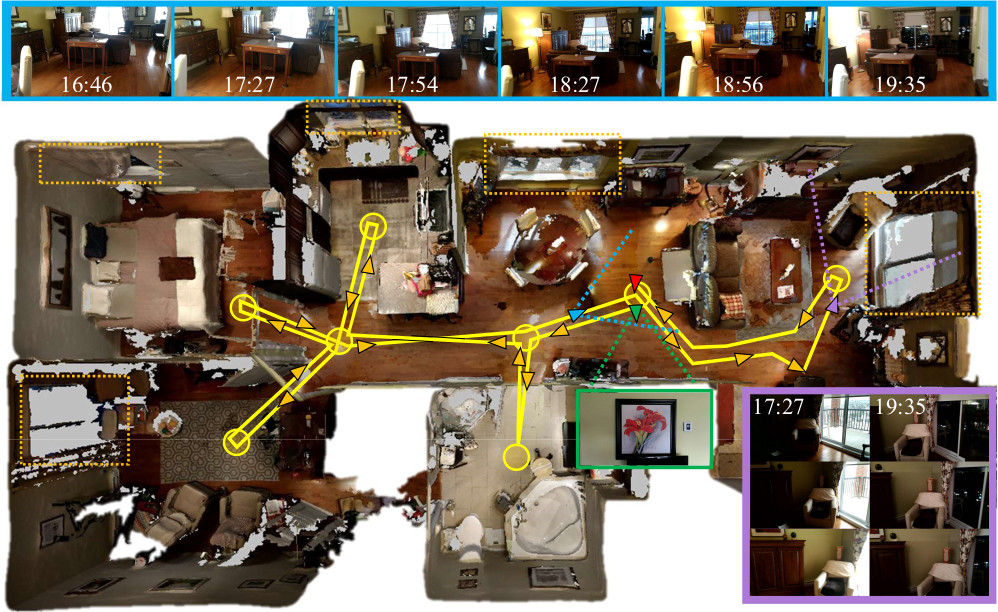
\includegraphics[width=100mm, keepaspectratio]{figures_jpg/rtabmap_for_applied_techs.jpg}
    \caption{RTAB-Map mapping process, source:~\cite{rtabmap_applied_techs}}
    \label{fig:rtabmap_applied_techs}
\end{figure}

RTAB-Map was introduced by Labbé and Michaud in 2013 as a solution to address the challenges of real-time 3D mapping. The core concept of RTAB-Map is to utilize an appearance-based loop closure detection method, which significantly enhances the robustness and accuracy of the mapping process. This method allows the system to recognize previously visited locations, thereby correcting the trajectory and reducing cumulative errors typically associated with SLAM algorithms.

One of the key features of RTAB-Map is its ability to handle large-scale environments. It achieves this by organizing the map into a graph structure where nodes represent keyframes, and edges represent spatial constraints between them. This graph structure is continuously optimized to improve the accuracy of the map and the estimated trajectory. Additionally, RTAB-Map employs a memory management strategy to keep the computational load manageable, ensuring that the system can operate in real-time even with extensive data.

RTAB-Map is highly versatile and supports various sensor configurations, including RGB-D cameras, stereo cameras, and LiDAR sensors. This flexibility makes it suitable for a wide range of applications, from indoor navigation to outdoor exploration. Moreover, RTAB-Map is integrated with ROS, providing a comprehensive suite of tools for robotic development and deployment. RTAB-Map has an iOS application too that works on iPhones which has LiDARs\footnote{\url{https://apps.apple.com/cd/app/rtab-map-3d-lidar-scanner/id1564774365}}.

\section{NVIDIA nvblox}

NVIDIA’s nvblox~\cite{nvblox_docs} is a GPU-accelerated spatial mapping library designed to work seamlessly with ROS2 and other robotics frameworks for real-time 3D environment reconstruction. Leveraging NVIDIA’s CUDA technology, nvblox processes data from depth sensors and LiDAR in real time, enabling robots to build and update dense 3D maps of their surroundings with low latency. Its main use cases include robotics applications requiring immediate spatial awareness, such as autonomous navigation, manipulation, and exploration in dynamically changing environments as seen on Figure~\ref{fig:nvblox_applied_techs}.

\begin{figure}[htbp]
    \centering
    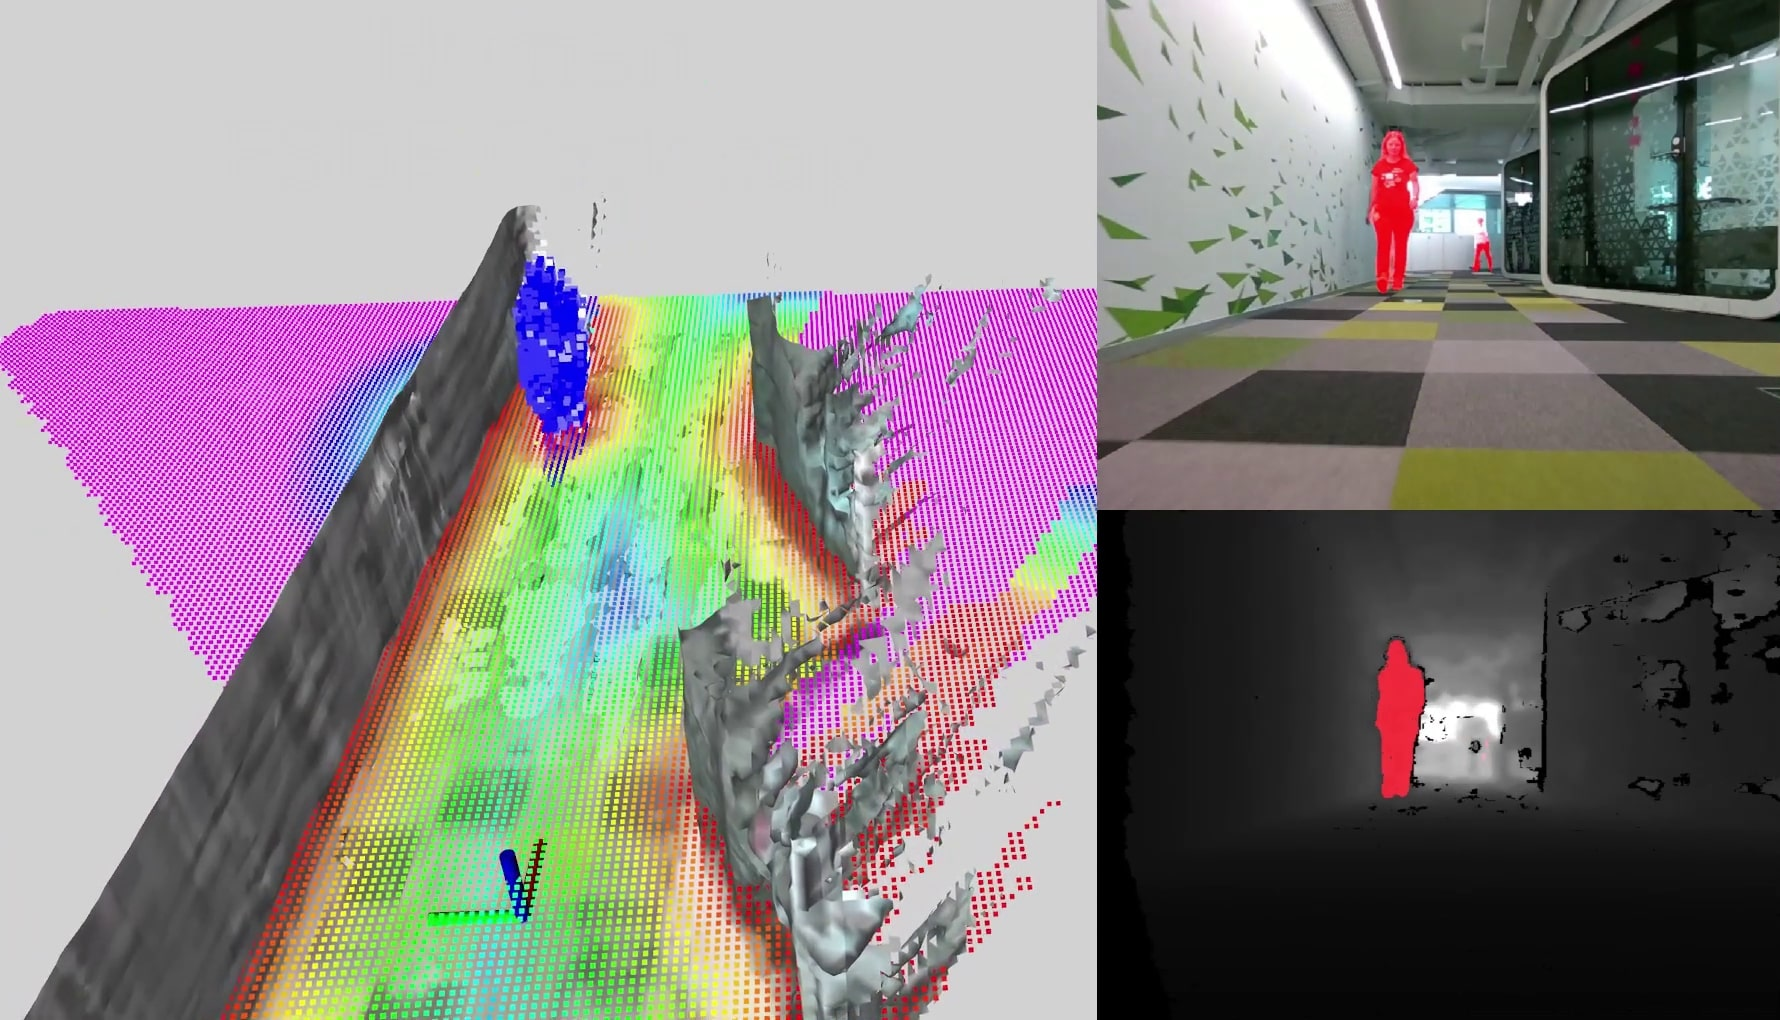
\includegraphics[width=100mm, keepaspectratio]{figures_jpg/nvblox_applied_techs.jpg}
    \caption{Nvblox exploration in dynamic environment, source:~\cite{nvblox}}
    \label{fig:nvblox_applied_techs}
\end{figure}

One of the key advantages of nvblox is its ability to generate high-resolution voxel grids and mesh representations at impressive speeds, a performance largely unattainable with CPU-only mapping solutions. A voxel map~\cite{voxelmap} is a 3D representation of an environment that divides the space into small, uniform cubes called voxels (volume elements), each storing spatial attributes such as occupancy, color, or surface normals. These attributes allow voxel maps to capture detailed environmental information in a compact and structured format, making them suitable for applications like navigation, object recognition, and path planning.

To enhance efficiency and scalability, some voxel mapping systems implement hierarchical voxel maps~\cite{hierarchical_voxelmap}, which organize voxels into a tree-like structure where finer detail is stored only in areas of interest. This hierarchical approach reduces memory usage and computational overhead by representing large, mostly empty spaces with coarser resolutions, while maintaining high-resolution detail in regions of complexity or activity.

Nvblox achieves its performance by maintaining and updating a voxel grid map. It also incorporates functionality to convert voxel maps into triangular meshes, which can then be visualized or further processed. With its ROS2 compatibility, nvblox can work as a ROS node, allowing direct integration with popular robotic systems and sensor data sources like RGB-D cameras, stereo cameras, and LiDAR, making it a practical solution for ROS-based projects.
Another significant feature of nvblox is its flexibility to run on various NVIDIA platforms, including Jetson devices, which are popular in edge computing and mobile robotics. This makes nvblox ideal for field applications where high-performance spatial understanding is critical. By reducing the computational load traditionally associated with real-time 3D mapping and enhancing efficiency, nvblox enables the creation of robust, high-fidelity maps that allow robots to react to and understand their environments effectively.

Despite its advantages, nvblox has certain drawbacks that make it challenging to deploy on resource-constrained platforms. In my experiments (see Section~\ref{experiments_nvblox}), I tested nvblox on my laptop with a GTX 1660 Ti GPU but found its performance to be inadequate due to the high computational demands. To run nvblox on the robot it should have a Jetson with 8 GB of VRAM but it only has a Raspberry Pi 4. While nvblox remains a promising tool for high-performance systems, these limitations restrict its use on platforms with limited computational resources.

\section{Neural reconstruction}

One of the various methods for neural reconstruction is Gaussian splatting~\cite{3DGS}. It is a rendering technique that offers a unique approach to representing and visualizing three-dimensional scenes. Instead of relying on traditional surface or line primitives to render objects, Gaussian splatting employs 3D ellipsoids with learnt parameters, which upon projecting to the image plane, produce "splats". These are essentially two-dimensional discs with Gaussian distribution characteristics. These splats are strategically placed within the scene based on key points extracted from images. By overlapping these splats, the technique reconstructs the underlying geometry and appearance of the scene.

One of the primary advantages of Gaussian splatting lies in its ability to faithfully capture the intricacies of complex scenes without requiring an explicit representation of geometry. This makes it particularly useful in scenarios where the scene's geometry is challenging to model or where the available data is sparse or noisy. By leveraging the information from multiple viewpoints, Gaussian splatting can generate detailed and coherent renderings, even from limited input data.

Recent advancements in the field, particularly in the realm of Neural Radiance Fields~\cite{nerf} (NeRFs), have propelled the development of photorealistic reconstruction techniques to new heights. NeRFs, which are neural network-based models capable of synthesizing novel views of a scene from a sparse set of input images, have demonstrated remarkable success in generating high-fidelity renderings. By using NeRFs, researchers have been able to achieve even more impressive results, enabling the generation of photorealistic renderings with enhanced efficiency and accuracy.

Gaussian splatting and NeRFs open up exciting possibilities for various applications, including virtual reality, augmented reality, computer graphics, and beyond. As research in this area continues to evolve, we can expect further innovations that push the boundaries of what is possible in three-dimensional scene reconstruction and rendering.

Gaussian Splatting has an original implementation which makes it easy to use\footnote{\url{https://github.com/graphdeco-inria/gaussian-splatting}}. I experimented with it during my thesis but with my GPU's memory limitations I could not be able to use it. Instead I used Nerfstudio's splatfacto model for experimenting with Gaussian splatting and the nerfacto model for experimenting with NeRFs. Nerfstudio makes it easy to create Gaussian splats or train NeRFs due to its user friendly CLI and the viser where I could examine the progress of the training. The Reader can examine these experiments more deeply in Chapter~\ref{nerf_gsplat}.

Our optional goal was to create photorealistic 3D models of the robot's environment from the images taken when mapping. This could be achieved with the help of Gaussian splatting. The result could be an environment's 3D model where we can place the robot's 3D model too and visualize its position real-time while it runs in localization mode using the discovered map.

To create a reconstructed map a dataset needs to be prepared for Nerfstudio. Images taken at keyframes are needed from the environment, then we need to estimate poses for these images with a photogrammetry software (like COLMAP), or the poses can be taken from SLAM directly (it is a more precise approach). In this thesis I will compare these approaches later on the evaluation in Chapter~\ref{evaluation}. Alongside with the images and poses a point cloud is also needed for the training, which can, again, be extracted from the SLAM process or can be estimated by a photogrammetry software. With the images, poses and point cloud the dataset is made and can be used by Nerfstudio for training. The training algorithm adjusts the NeRF's weights/Gaussian splatting parameters making the model to represent the input scene precisely. At the end, a scene can be rendered from the trained NeRF or a splat can be exported from the Gaussians.

\chapter{Experiments in RGBD sensing using DepthAI} \label{experiments_oak_d}

\section{Overview}

%In this chapter, we present the design and implementation of our solution, focusing on visual mapping and 3D reconstruction. The experiments and methodologies employed in this thesis aim to evaluate the performance and capabilities of various tools and techniques for real-time mapping and object detection.

In this chapter we explore the capabilities of the OAK-D camera using the DepthAI Viewer software to understand its functionalities. This exploration provided insights into the camera's real-time 3D reconstruction and its Vision Processing Unit (VPU) capabilities. Subsequently, we experimented with the Spectacular AI SDK to further test the camera's performance, especially in mapping and person detection scenarios.

%%% Overall, this chapter provides a comprehensive overview of the experimental design, methodologies, and outcomes of our efforts to develop an effective solution for real-time mapping and 3D reconstruction using state-of-the-art technologies.

\section{DepthAI Viewer}

To begin exploring the capabilities of the camera, I initiated my efforts by testing the example software provided by the camera's manufacturer, namely DepthAI Viewer\footnote{\url{https://github.com/luxonis/depthai-viewer}}. This software proved invaluable for its ability to showcase the camera's functionalities effectively.

Upon installation, I gained access to a user-friendly interface that allowed me to view images captured by the camera in real time. Additionally, the software facilitated real-time 3D reconstruction of the camera's surroundings, as depicted in Figure~\ref{fig:DAI_3d}. Notably, the DepthAI Viewer leveraged the Vision Processing Unit (VPU) embedded within the device, thereby enabling comprehensive exploration of its capabilities, as illustrated in the top left corner of Figure~\ref{fig:DAI_person_detection}.

\begin{figure}[htbp]
	\centering
	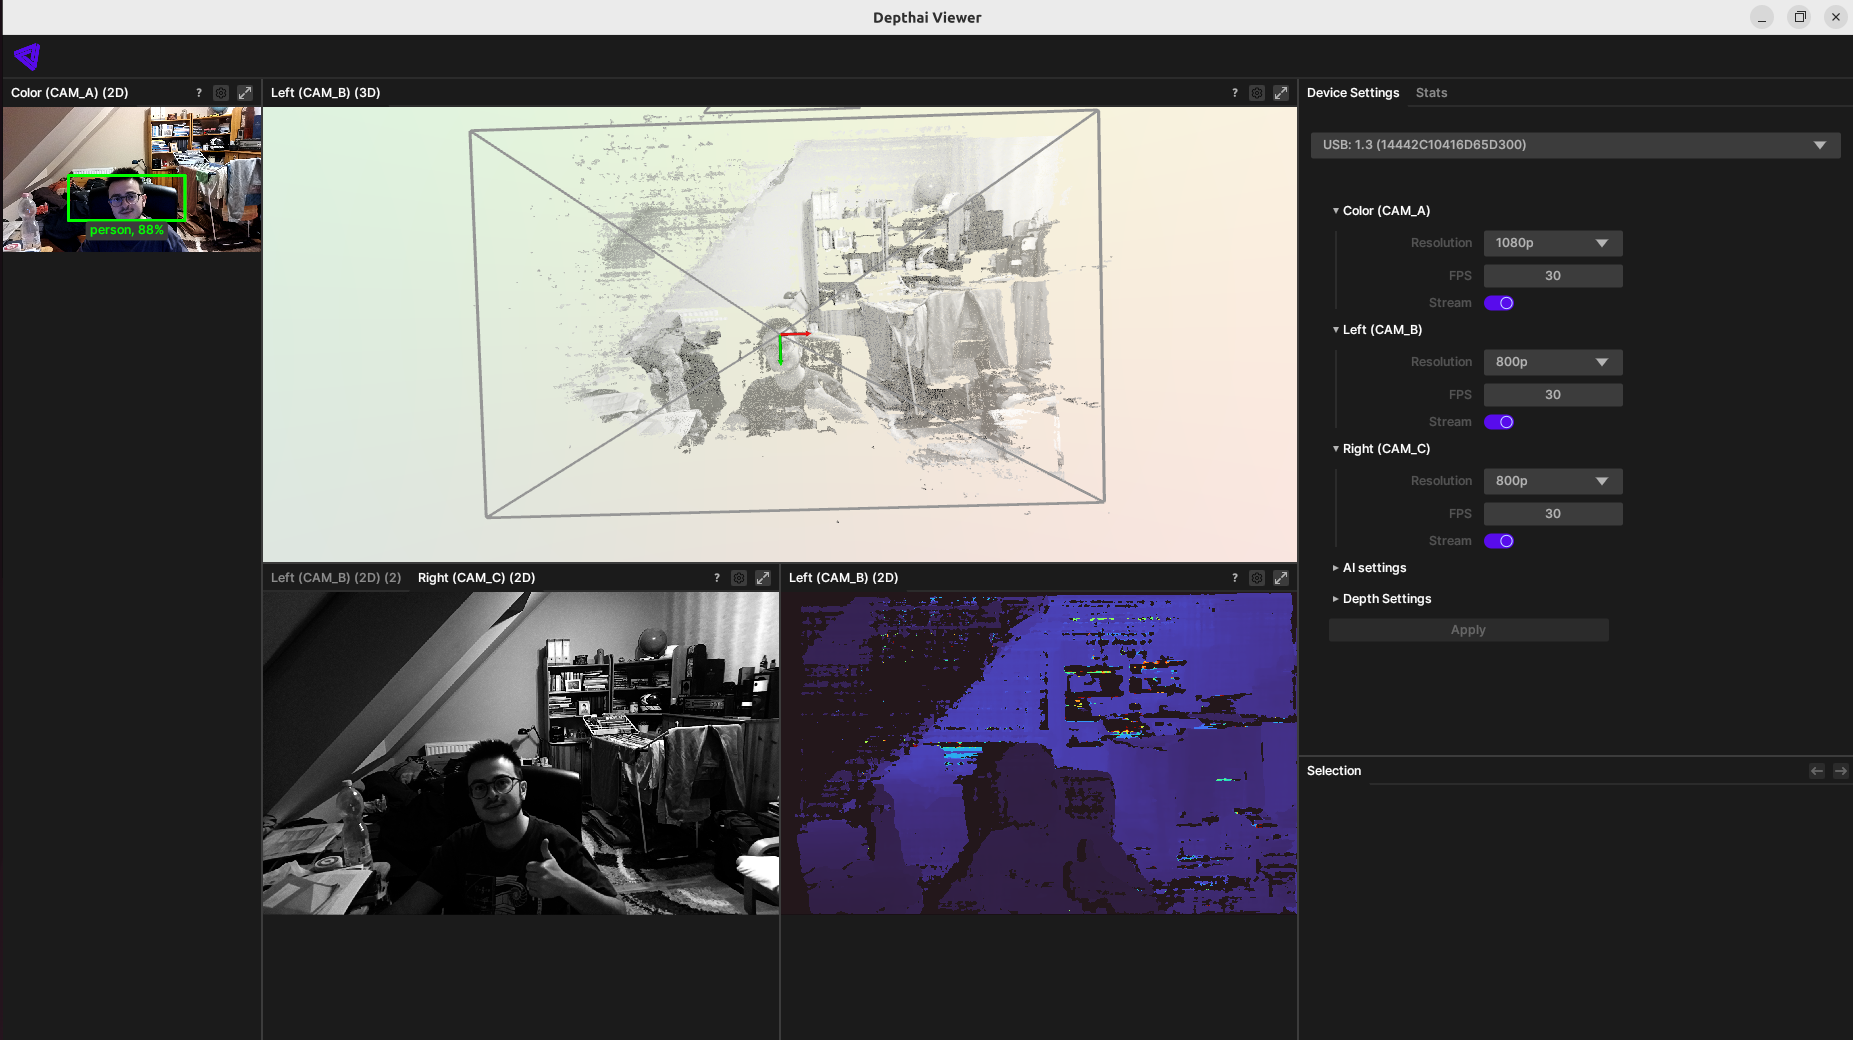
\includegraphics[width=150mm, keepaspectratio]{figures/depthai_viewer.png}
	\caption{DepthAI Viewer with person detection}
	\label{fig:DAI_person_detection}
\end{figure}

\begin{figure}[htbp]
	\centering
	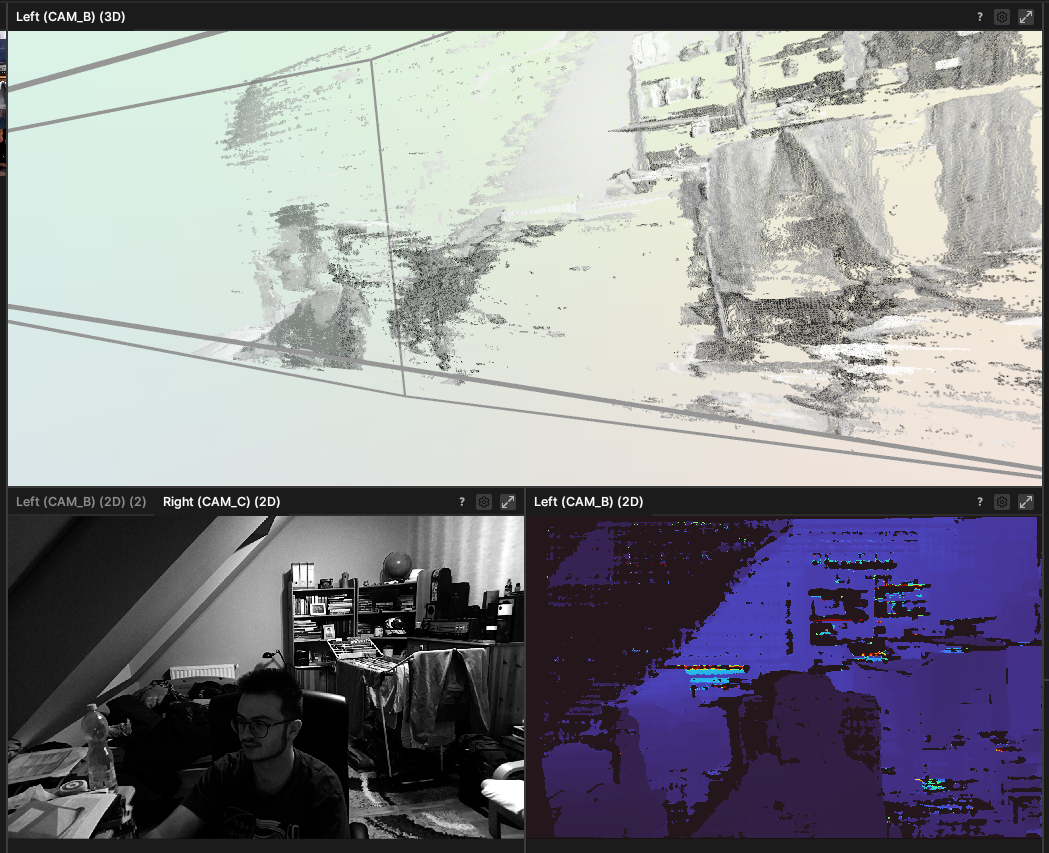
\includegraphics[width=150mm, keepaspectratio]{figures/depthai_viewer_3d.png}
	\caption{DepthAI Viewer's 3D reconstruction}
	\label{fig:DAI_3d}
\end{figure}

This initial exploration served as a foundational step in understanding the camera's capabilities and paved the way for further experimentation and development in subsequent tasks.


\section{Experimenting with Spectacular AI} \label{experiments_spai}

The next step was to experiment with the Spectacular AI SDK's examples to determine if it is capable of mapping and detecting persons with low latency. At first the Python scripts threw a warning and they did not work: 
\FloatBarrier
\begin{lstlisting}[language=bash,frame=single,float=h]
SpectacularAI WARN: Dropping frames!
SpectacularAI WARN: VIO may be running too slow, data is being input too fast, or IMU samples are missing / time-offset from frames. (buffer size 10)
\end{lstlisting}
After some research, I found out that this problem is related to outdated firmware version on the camera (note that it took a long time to find the solution due to the severe lack of documentation). To solve the issue, Luxonis' \verb|depthai-python| repo\footnote{\url{https://github.com/luxonis/depthai-python}} must be cloned and the IMU firmware update script\footnote{\url{https://github.com/luxonis/depthai-python/blob/main/examples/IMU/imu_firmware_update.py}} must be ran. After the successful firmware update I was able to try out the examples.

The simplest example is the one that visualizes the camera's movement. It extracts the data from the IMU and uses matplotlib for visualization. As we can see on Figure \ref{fig:IMU_visu}, I was able to draw a heart in the air. The curves are not perfect because my hand was probably shaking a bit.

\begin{figure}[htbp]
	\centering
	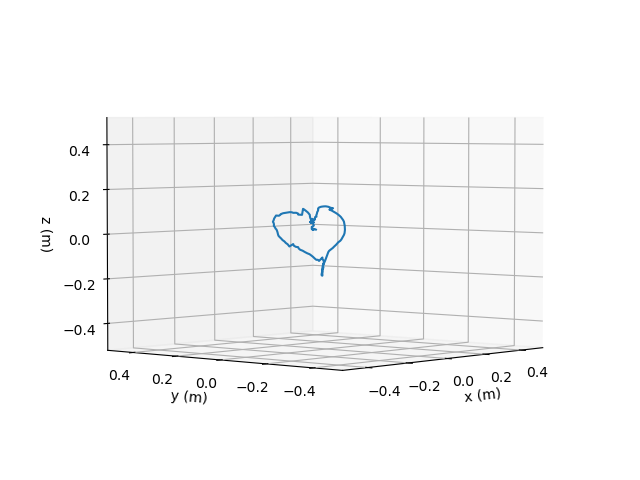
\includegraphics[width=150mm, keepaspectratio]{figures/spectacular_ai_vio_visu.png}
	\caption{IMU visualization with Spectacular AI}
	\label{fig:IMU_visu}
\end{figure}

A bit more advanced example uses the camera too, not just the IMU. When the camera is covered with our hand it visualizes the device's movement with the help of the IMU as we can see on Figure \ref{fig:3d_pen}.

\begin{figure}[htbp]
	\centering
	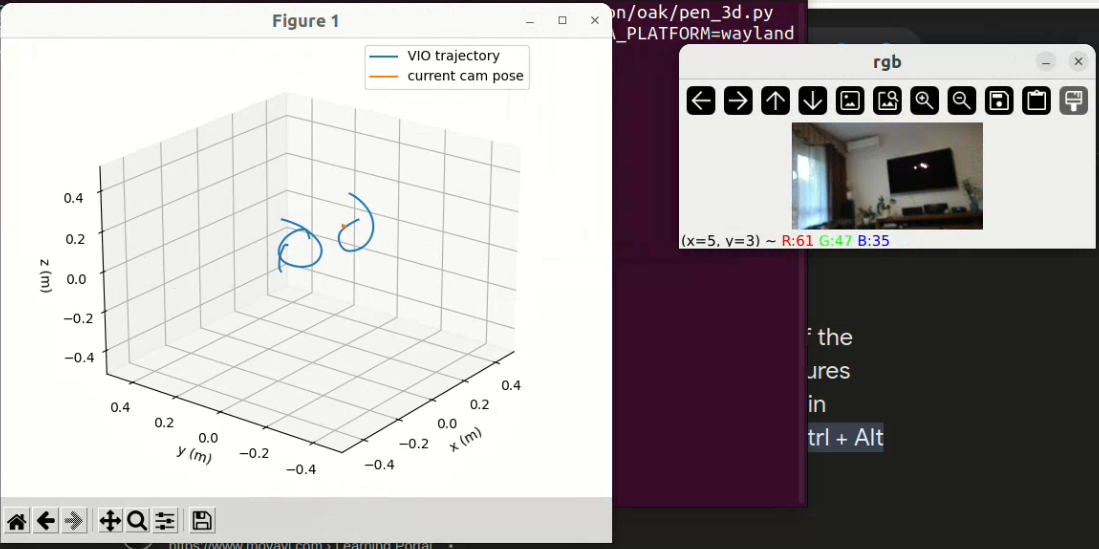
\includegraphics[width=150mm, keepaspectratio]{figures/3d_pen.png}
	\caption{IMU visualization with Spectacular AI}
	\label{fig:3d_pen}
\end{figure}

These examples just visualized the camera's movement and the picture taken with the camera so we did not see any mapping or person detection yet. The repository fortunately provides some spectacular examples on these applications too. However these examples always raised an error which had to be debugged. These examples use OpenGL for visualization and the problem stood in some deep OpenGL code. The easiest way to solve this problem was to comment out some code in \verb|OpenGL/contexdata.py|:

\begin{lstlisting}[language=python,frame=single,float=!ht]
def getContext( context = None ):
    """Get the context (if passed, just return)
    context -- the context ID, if None, the current context
    """
    if context is None:
        context = platform.GetCurrentContext()
    # if context == 0:
        # from OpenGL import errorS
        # raise error.Error(
        # """Attempt to retrieve context when no valid context"""
        # )
    return context
\end{lstlisting}
\FloatBarrier

We can try out some mapping applications, such as point cloud mapping (Figure~\ref{fig:SPAI_mapping}), real-time AR mapping with mesh (Figure~\ref{fig:SPAI_mesh_mapping}), real-time AR mapping with point cloud (Figure~\ref{fig:SPAI_point_cloud_mapping}) and mapping with ROS2 integration (Figure~\ref{fig:SPAI_ros_mapping}).

\begin{figure}[htbp]
	\centering
	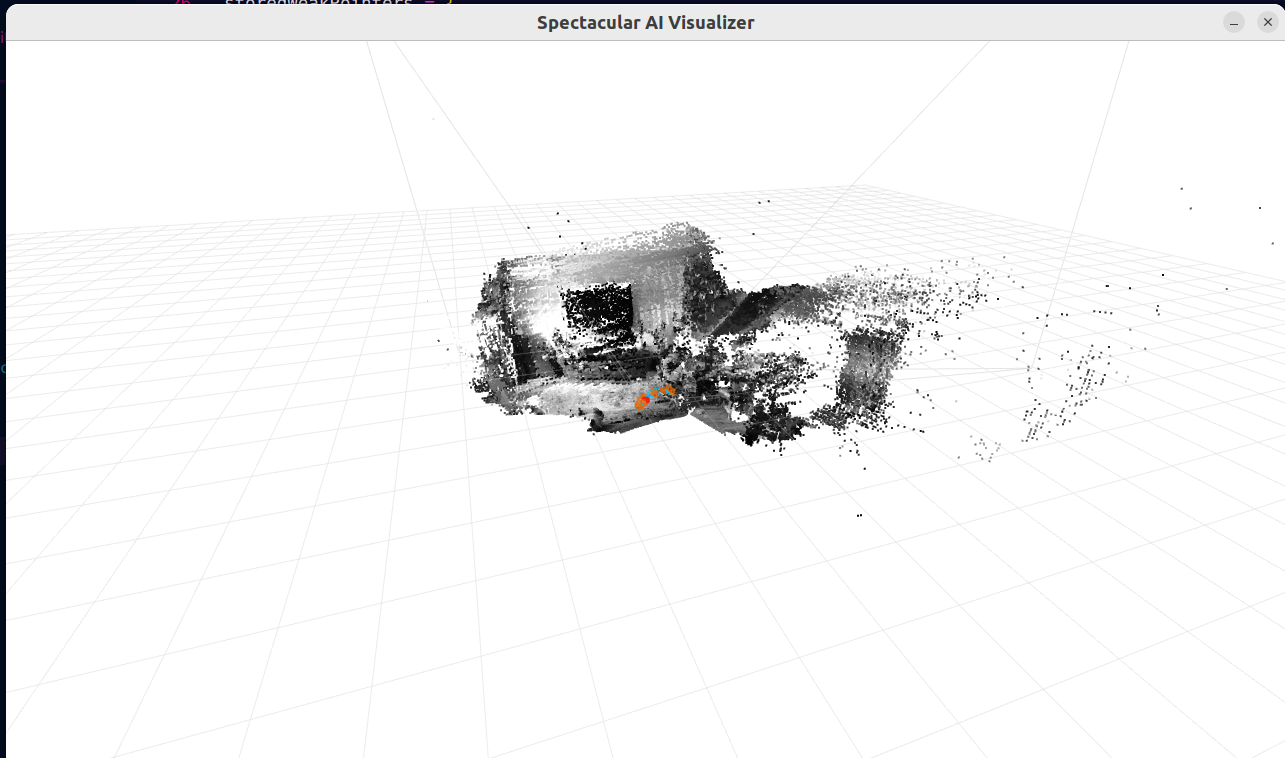
\includegraphics[width=150mm, keepaspectratio]{figures/spectacular_ai_mapping_visu.png}
	\caption{Mapping with Spectacular AI}
	\label{fig:SPAI_mapping}
\end{figure}

\begin{figure}[htbp]
	\centering
	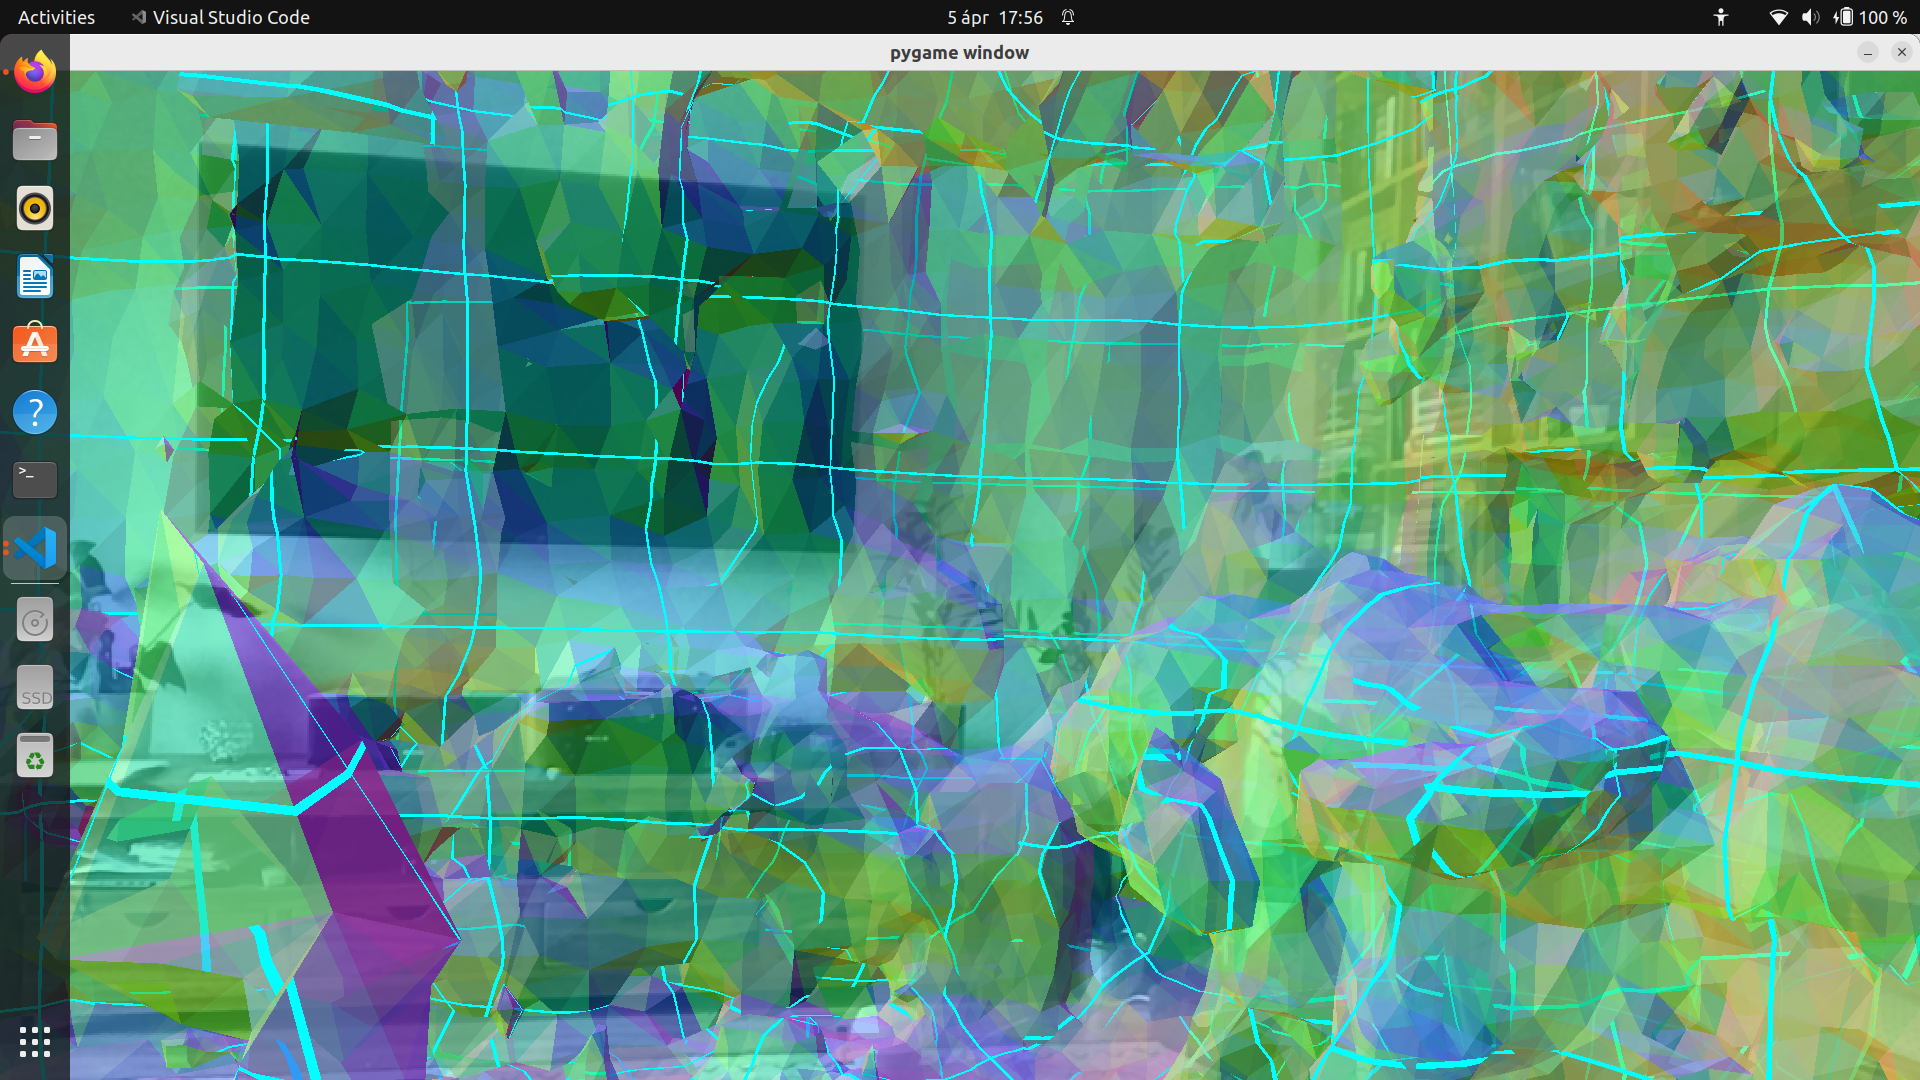
\includegraphics[width=67mm, keepaspectratio]{figures/spectacular_ai_mapping_ar_mesh1.png}\hspace{1cm}
	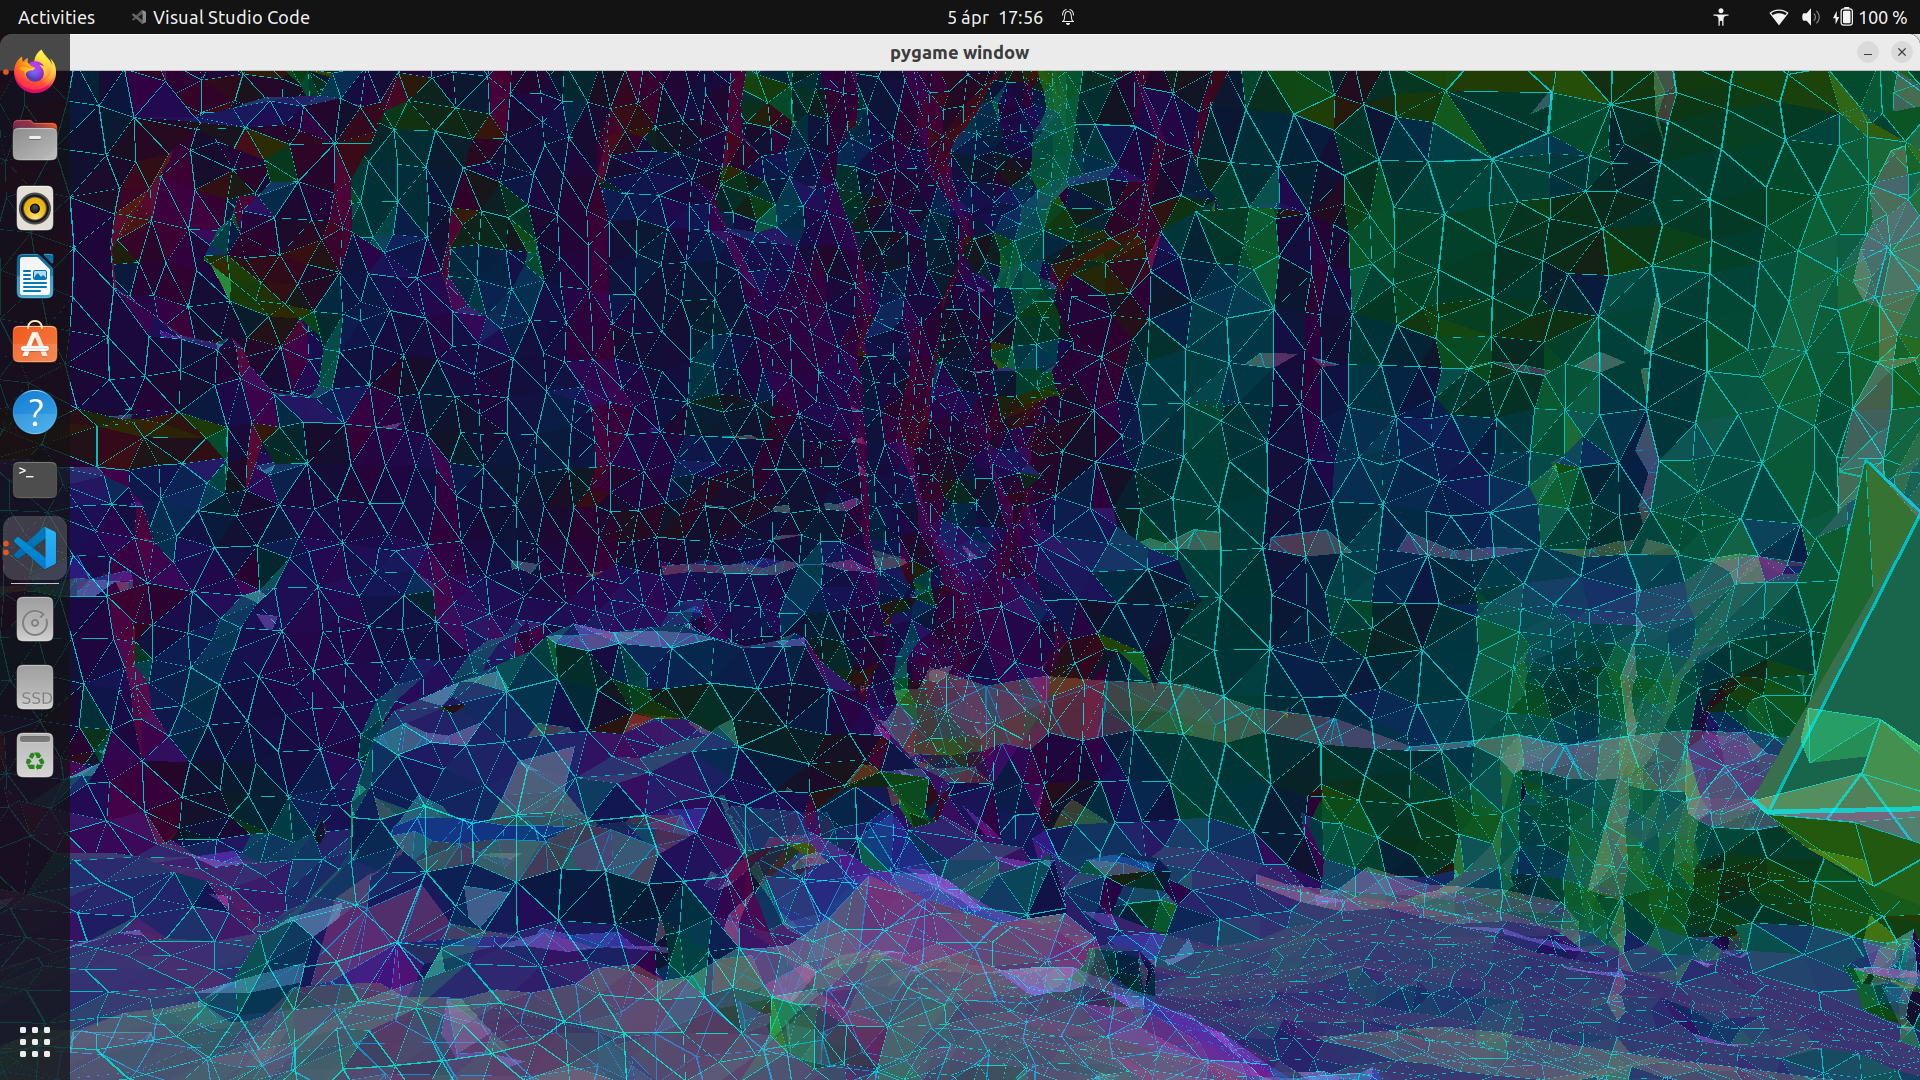
\includegraphics[width=67mm, keepaspectratio]{figures/spectacular_ai_mapping_ar_mesh2.png}\\\vspace{5mm}
	\caption{AR mesh mapping with Spectacular AI}
    \label{fig:SPAI_mesh_mapping}
\end{figure}

\begin{figure}[htbp]
	\centering
	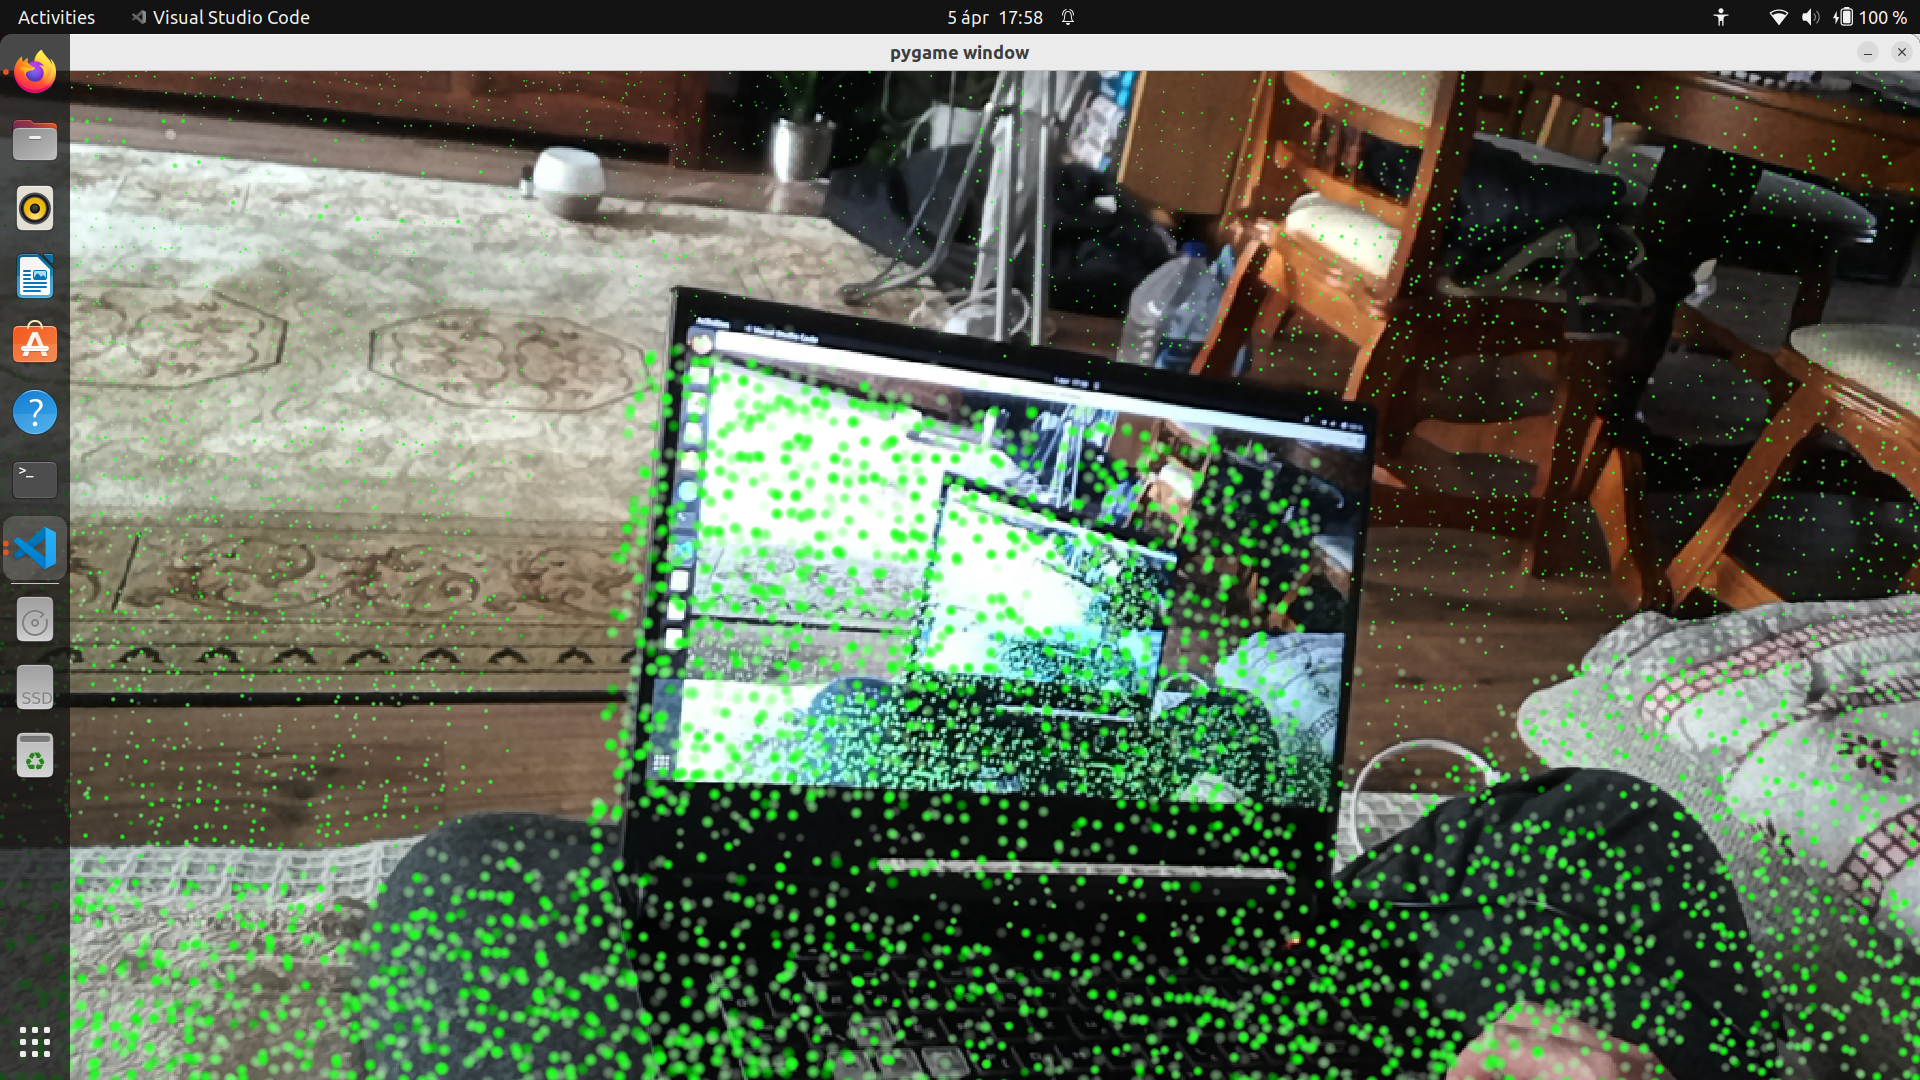
\includegraphics[width=67mm, keepaspectratio]{figures/spectacular_ai_mapping_ar_pc1.png}\hspace{1cm}
	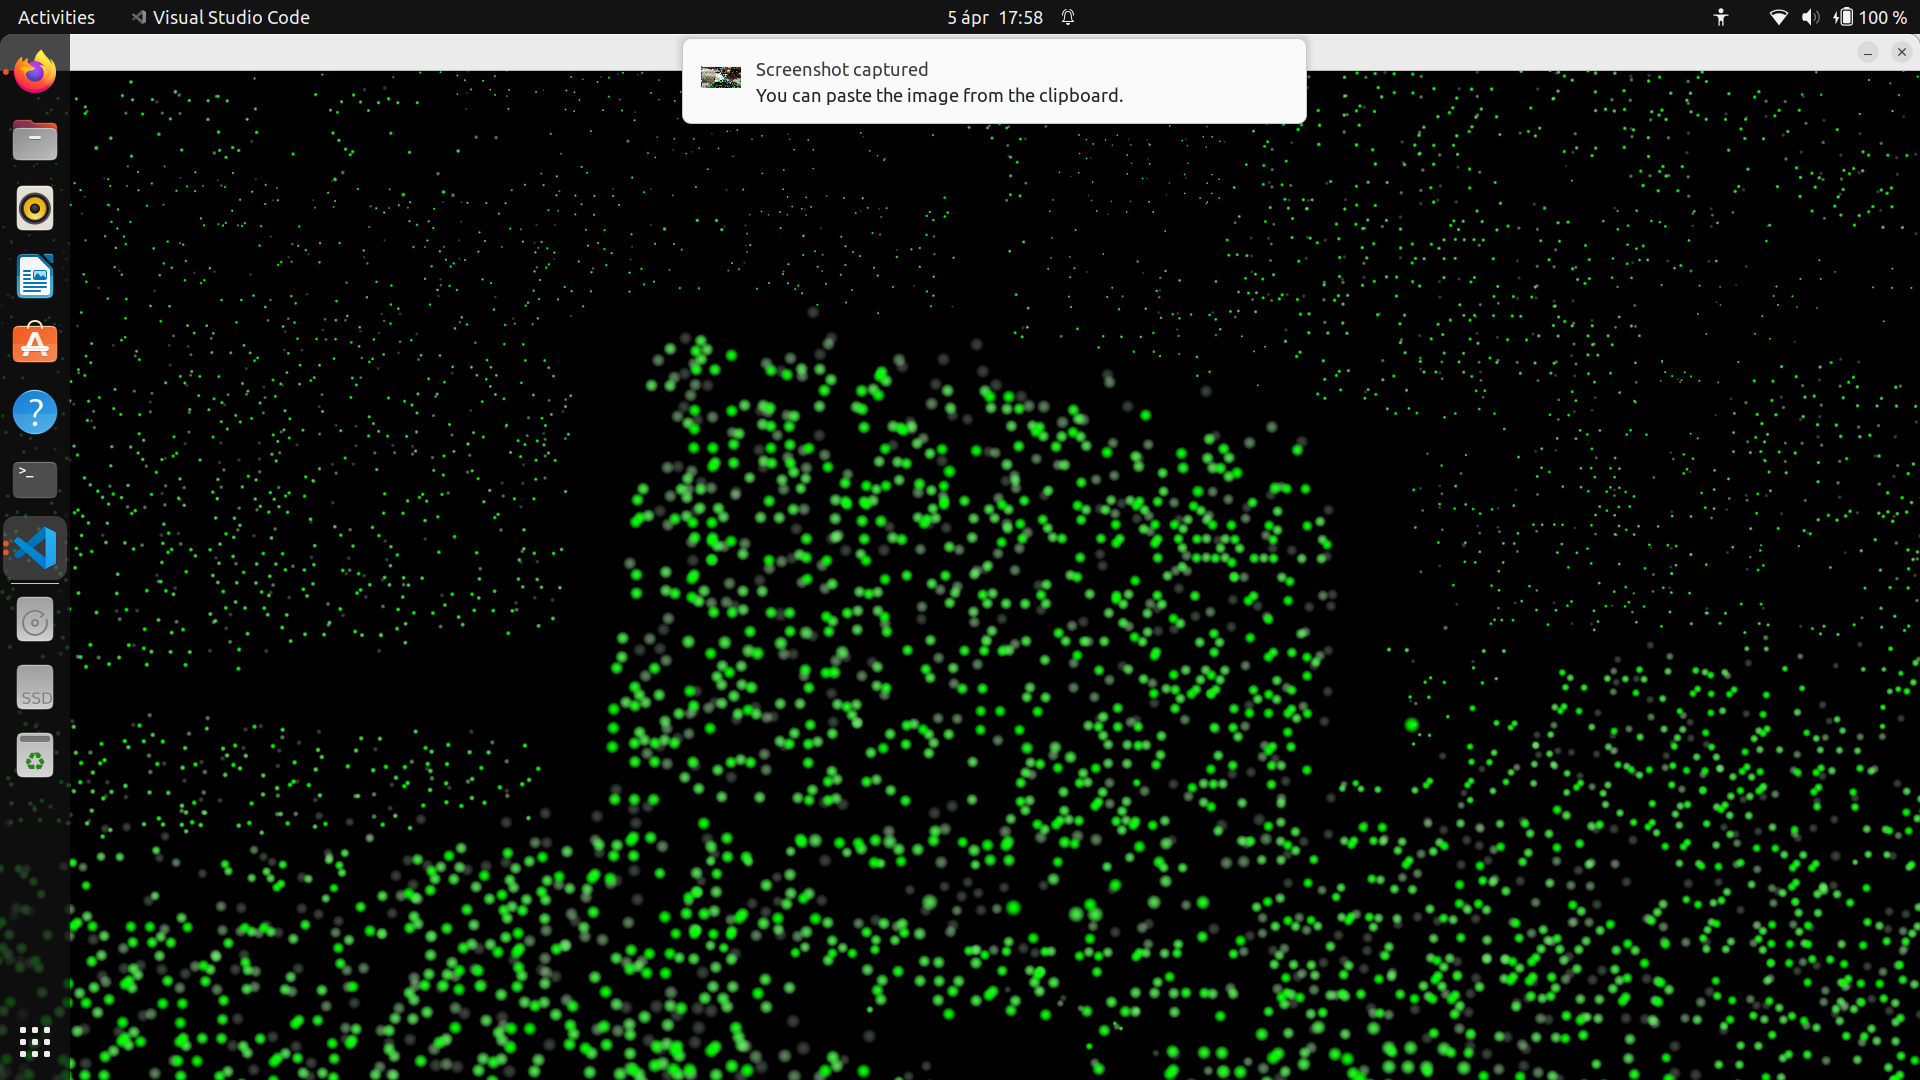
\includegraphics[width=67mm, keepaspectratio]{figures/spectacular_ai_mapping_ar_pc2.png}\\\vspace{5mm}
	\caption{AR point cloud mapping with Spectacular AI}
    \label{fig:SPAI_point_cloud_mapping}
\end{figure}

\begin{figure}[htbp]
	\centering
	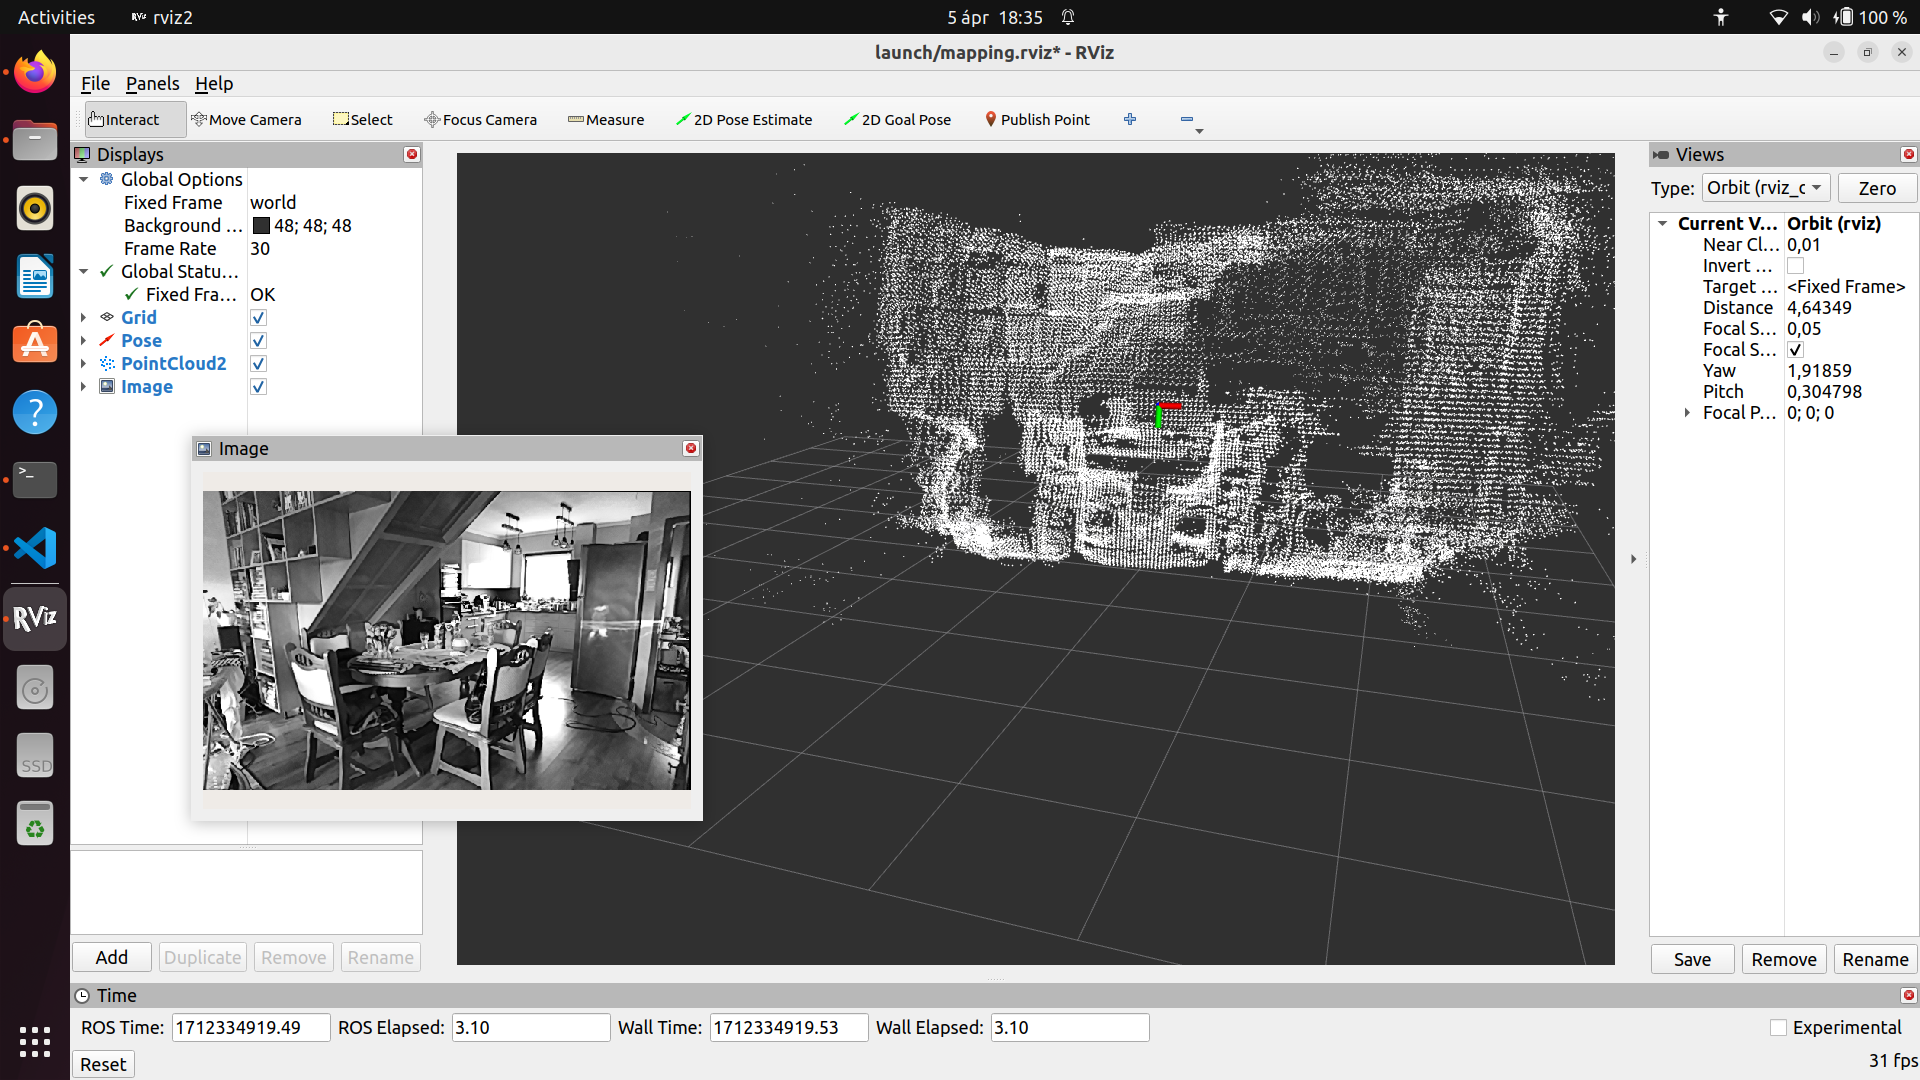
\includegraphics[width=150mm, keepaspectratio]{figures/spectacular_ai_mapping_ros2.png}
	\caption{ROS2 mapping with Spectacular AI}
	\label{fig:SPAI_ros_mapping}
\end{figure}

As we can see, the Spectacular AI SDK works really well with the OAK camera. During the testing of the examples, I could not experience any major latencies so we can safely say that it works in real time.

I saved the most exciting example for the last one of each. As I said earlier, the camera contains a VPU (Intel Movidius Myriad X\footnote{\url{https://www.intel.com/content/www/us/en/products/sku/204770/intel-movidius-myriad-x-vision-processing-unit-0gb/specifications.html}}) which can run neural network models. We do not have to make any post-processing or post-detecting with neural networks because it can be ran on the camera itself. Thanks to the stereo cameras and the VPU, the OAK-D is able to detect objects and calculate their location on the fly. To select what type of objects we want to detect, we have to modify the example code (we only have to modify one list). As we can see on Figure~\ref{fig:SPAI_depthai}, I customised the code to detect potted plants in the living room. Due to inadequate lighting the detections did not perform 100\% but they are acceptable. Moreover, I measured the positions of the plants myself and I can safely say that the camera calculated the distances really accurately.

\begin{figure}[H]
	\centering
	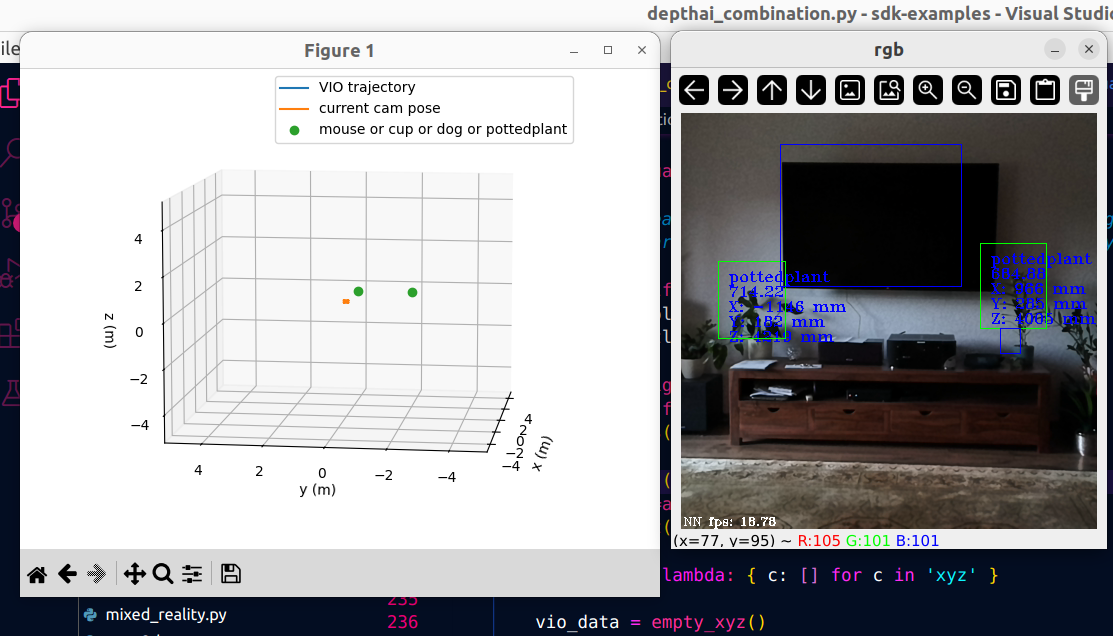
\includegraphics[width=150mm, keepaspectratio]{figures/spectacular_ai_depthai_combination.png}
	\caption{Spectacular AI's object detection and position calculation}
	\label{fig:SPAI_depthai}
\end{figure}

\GS{describe here that if we can track the camera pose in the room using SPAI and we can detect objects with depth in 3D on any camera image, that means we can detect the 3D position of objects within the room! This will be important for the mapping.}

\section{Experimenting with a custom person detector}

It was one of our goals to detect persons with the camera and make the robot follow or avoid them while mapping. For that purpose we first tried out the Spectacular AI's example on the robot's camera but we soon realized that the position of it is not ideal for detecting objects. Due to the platform above the robot it limits the FOV (Field of View) of the camera so much that if we stood 2-3 meters away from the robot only our legs were visible, thus the detection was not working. Our solution for this problem was to put the camera right at the front of the platform with some plasticine and it caused the FOV to be increased. The detection of my advisor with the camera at front can be seen on Figure \ref{fig:person_detection_camera_at_front_nokia} (the other detected person is a woman on a poster).

\begin{figure}[htbp]
    \centering
    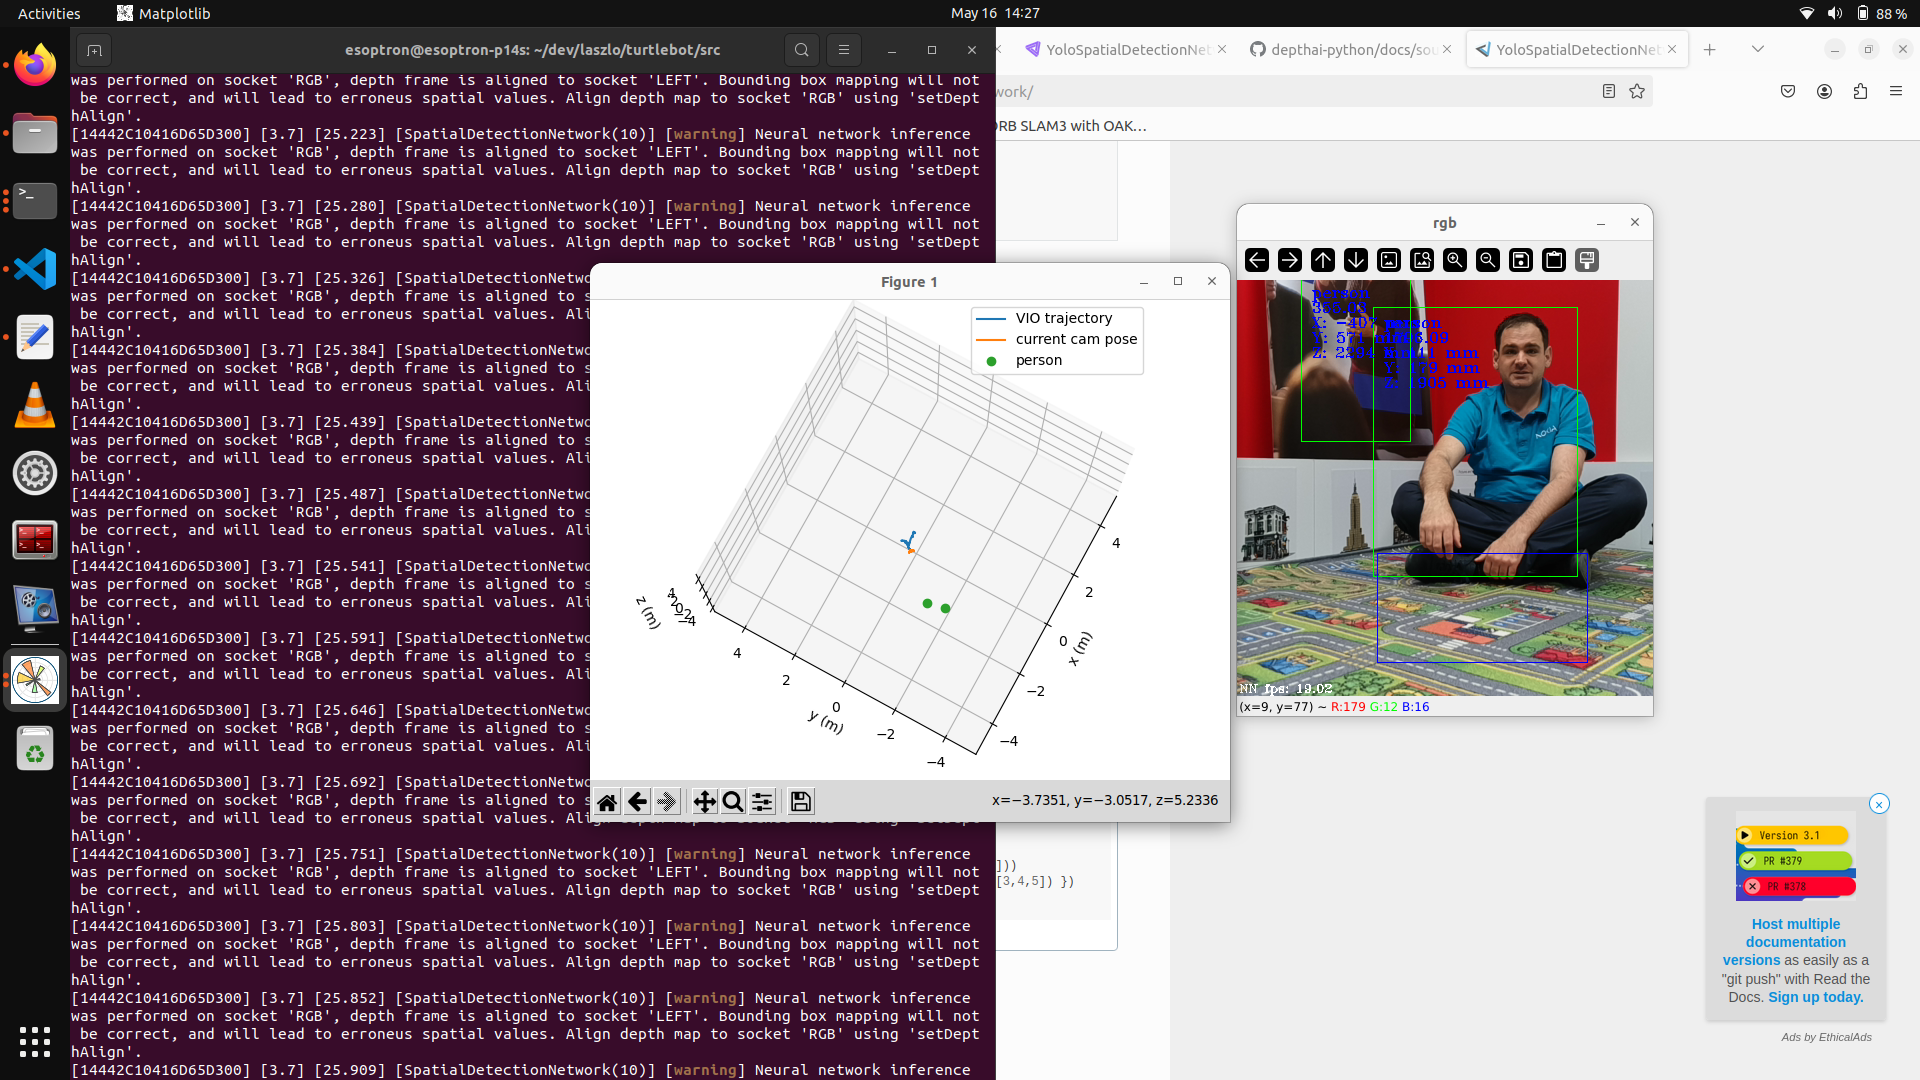
\includegraphics[width=150mm, keepaspectratio]{figures/person_detection_camera_at_front_nokia.png}
    \caption{Person detection with the camera at front at Nokia Bell Labs}
    \label{fig:person_detection_camera_at_front_nokia}
\end{figure}

After we experimented with the FOV and the example detection script I created a custom script based on the example which uses the camera to detect persons and publish their location in world coordinates on a ROS topic (the code can be examined at \ref{custom_person_detector}). The base example and my custom person detector froze after some detections with an error indicating that the IMU buffer size is exceeded. It happens because the IMU sends data too rapidly, the configuration of the \verb|SpatialLocationCalculator| node uses a buffer that is too small for storing that much data and, on top of that, it does not flush the buffer frequently enough. That buffer cannot be extended or flushed because it is fixed in the aforementioned node. In conclusion, we could not implement a stable person detection using this camera due to its previously stated limitations.

\chapter{Experiments with neural reconstruction} \label{nerf_gsplat}

\section{Overview}

%We explored advanced techniques for generating photorealistic 3D models of the robot's environment. This involved leveraging Neural Radiance Fields (NeRFs) and Gaussian Splatting to create realistic simulations of the robot's surroundings. These techniques were evaluated using various tools, including Nerfstudio, Gaussian Splatting and Luma AI, to determine their feasibility and performance in generating accurate 3D reconstructions.

An additional objective we pursued was to generate 3D photorealistic models of the robot's environment, leveraging images captured during the mapping process. Upon completion of mapping, our aim was to seamlessly integrate the robot's 3D model into this reconstructed scene. This integration would enable real-time simulation of the robot's movements during localization, transcending beyond a mere representation with a point cloud to deliver a highly realistic simulation experience.

\section{Using Spectacular AI to create input for NeRFs}

Continuing my exploration, I delved into the realm of 3D reconstruction using Neural Radiance Fields (NeRFs)~\cite{nerf}. To initiate this process, I utilized an example provided by the Spectacular AI SDK, specifically the \verb|mapping_visu.py| script. This script facilitated the creation of a mapping video, allowing for the specification of an output folder to store both the captured videos from the camera(s) and the resulting point cloud.

\begin{lstlisting}[language=bash,frame=single,float=!ht]
$ python3 mapping_visu.py --recordingFolder /PATH/TO/FOLDER
\end{lstlisting}

We have made significant progress, now possessing videos and a point cloud. However, these resources alone don't suffice as input for NeRFs, which demand a more specific format. NeRFs require not only the images captured at keyframes but also a COLMAP, which contains essential information about the camera setup.

Keyframes serve as pivotal snapshots within the video sequence, capturing unique elements from various perspectives. These frames are crucial for determining the precise position and orientation of the camera at different points in the scene. Drawing a parallel from the animation realm\cite{keyframes_in_animation}, keyframes are akin to markers that delineate significant moments or transitions between actions. In our context, these actions translate to movements such as forward progression or changes in direction.

Additionally, the COLMAP plays a pivotal role by providing foundational data about the camera configuration, including camera positions within each image and a point cloud derived from the scene mapping process\cite{colmap}. This comprehensive dataset serves as the backbone for NeRFs, enabling them to synthesize realistic renderings by leveraging both visual information and spatial context.

By integrating keyframes and COLMAP data, we can create a robust input pipeline for NeRFs, facilitating the generation of immersive and accurate 3D reconstructions from our captured videos and point cloud.

The long-discussed conversion can be done with the help of another Spectacular AI tool, called \verb|sai-cli|. It is a command line tool that can capture videos from OAK cameras and can execute the conversion for NeRF inputs. The required command for creating the input dataset for NeRFs is as follows:

\FloatBarrier
\begin{lstlisting}[language=bash,frame=single,float=!ht]
$ sai-cli process --format FORMAT --preview --preview3d INPUT OUTPUT
\end{lstlisting}

The execution of the command can be observed on Figure \ref{fig:sai_cli_process}. 

\begin{figure}[htbp]
	\centering
	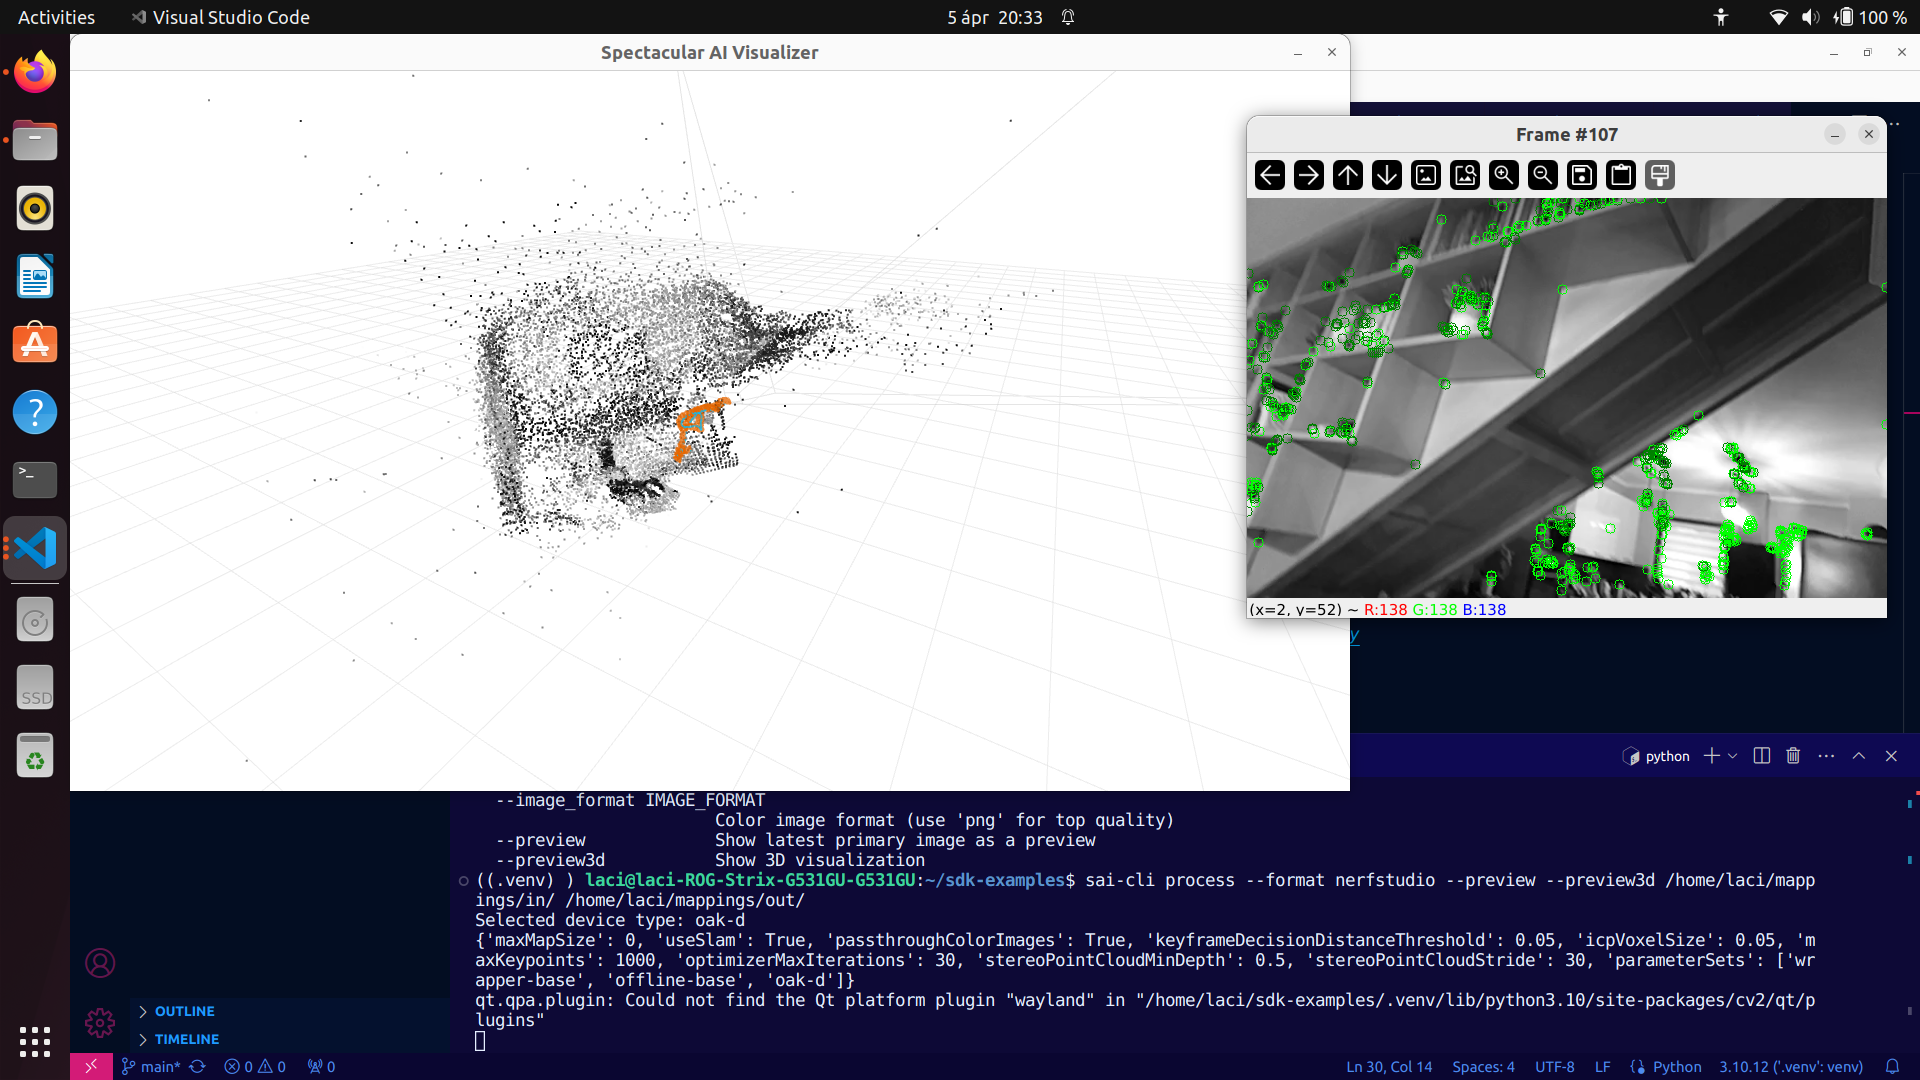
\includegraphics[width=150mm, keepaspectratio]{figures/sai-cli_process.png}
	\caption{Spectacular AI's CLI tool for creating input for NeRFs}
	\label{fig:sai_cli_process}
\end{figure}

\section{Experimenting with nerfstudio}

With the created input the only thing that stops us from training a NeRF is installing a tool for it. For training I used Nerfstudio\cite{nerfstudio} but due to constant errors during installation with conda I switched to a simpler solution: Docker\footnote{\url{https://www.docker.com/}}. While browsing through the Docker images on DockerHub\footnote{\url{https://hub.docker.com/}}, I experienced that the official Docker image of nerfstudio (nerfstudio/nerfstudio\footnote{\url{https://hub.docker.com/r/nerfstudio/nerfstudio}}) is badly maintained: it is rarely updated and the tagging is unacceptable (the only tag of the image is \verb|latest| so we are unable to pull earlier versions of it)... Thankfully I found a more well-maintained image (dromni/nerfstudio\footnote{\url{https://hub.docker.com/r/dromni/nerfstudio}}) which is updated regularly and tagged professionally.

The Docker container can be started with the following command (I mounted the folders containing the inputs, gave permission for the container to use GPU, specified the user and increased the shared memory which the container can use):

\FloatBarrier
\begin{lstlisting}[language=bash,frame=single,float=!ht]
$ sudo docker run --gpus all \
    -u $(id -u) \
    -v /home/laci/mappings/:/workspace/ \
    -v /home/laci/.cache/:/home/user/.cache \
    -p 7007:7007 --rm -it \
    --shm-size=1gb \
    dromni/nerfstudio:main
\end{lstlisting}

The training can be started inside the container with the following command:
\FloatBarrier
\begin{lstlisting}[language=bash,frame=single,float=!ht]
$ ns-train nerfacto --data PATH_TO_DATA
\end{lstlisting}
It is worth mentioning that nerfstudio has many trainable NeRF models, but for the sake of simplicity I sticked with the one mentioned in the quickstart guide\footnote{\url{https://docs.nerf.studio/quickstart/first_nerf.html}}, which is called nerfacto. The training process and a part of the trained model can be seen on Figure \ref{fig:training_nerf_karcag} and Figure \ref{fig:trained_nerf_karcag}.

\begin{figure}[htbp]
	\centering
	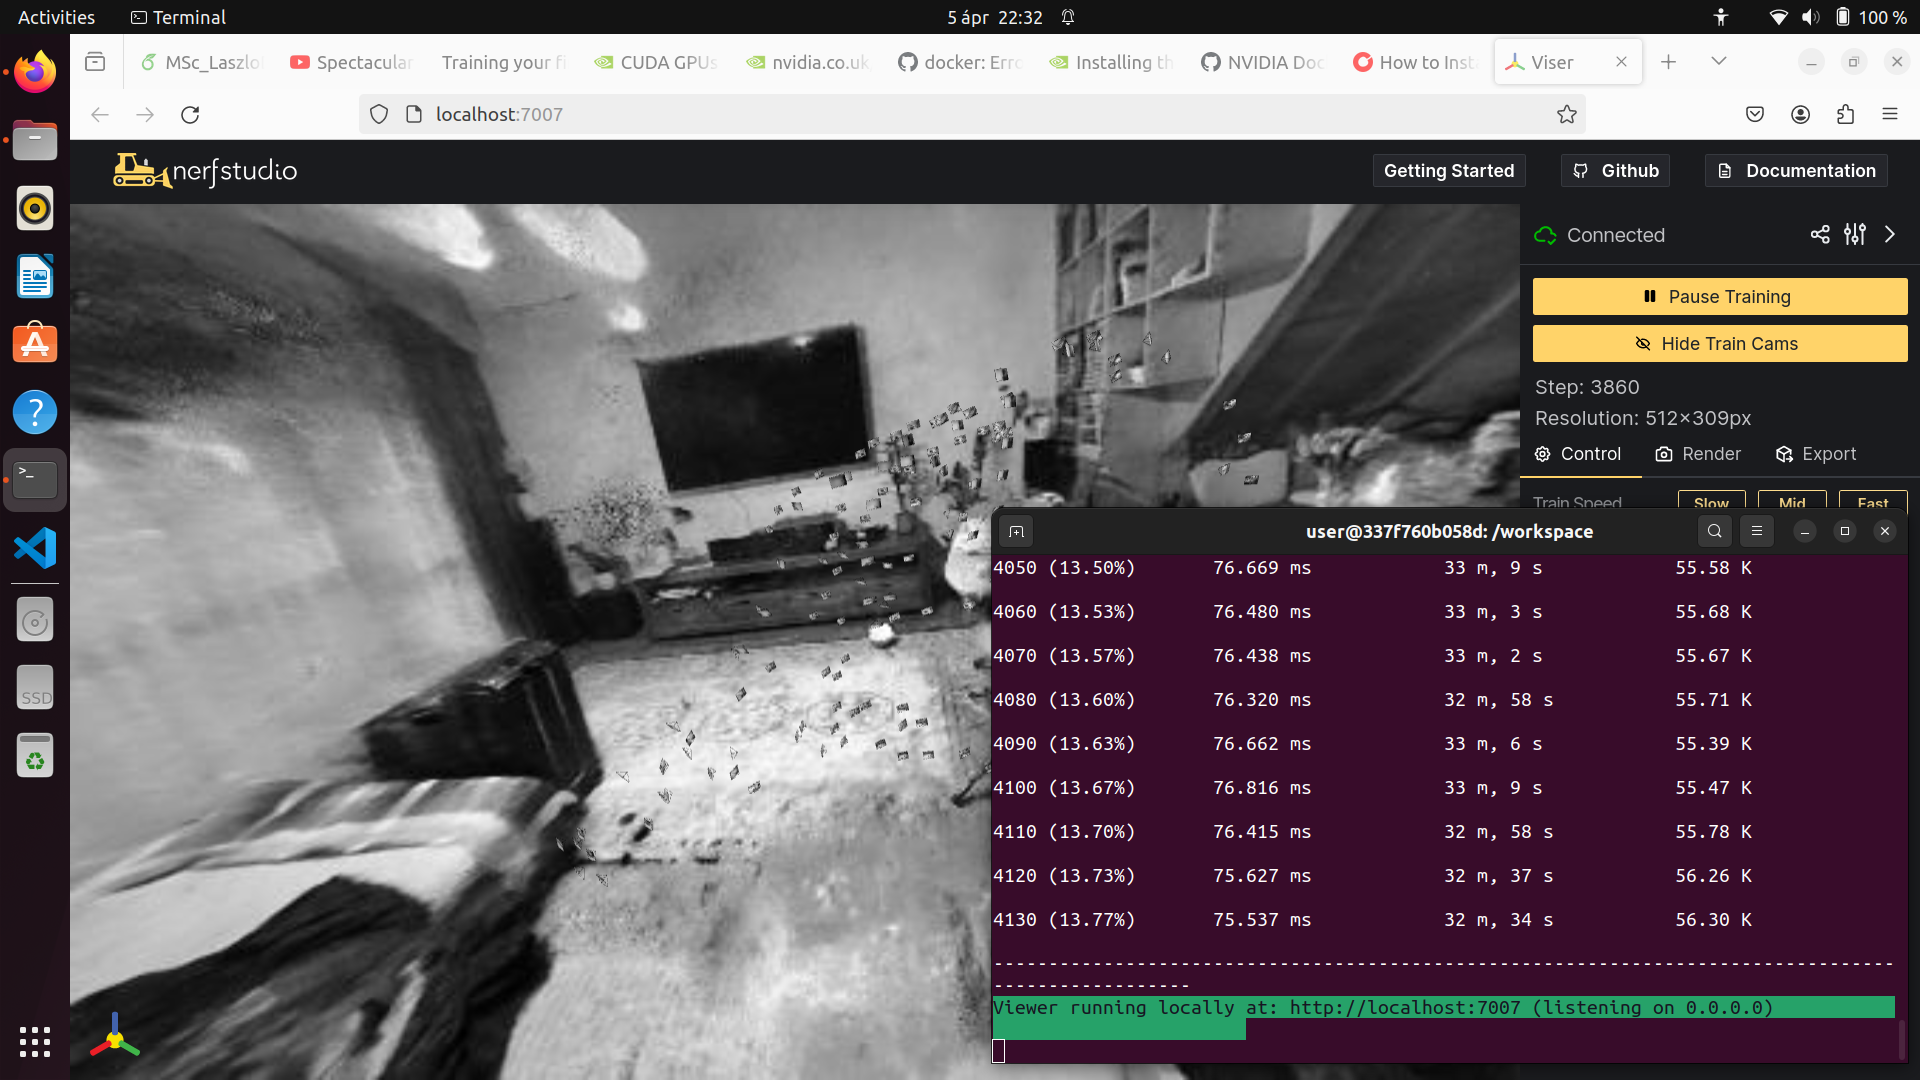
\includegraphics[width=150mm, keepaspectratio]{figures/nerfstudio.png}
	\caption{Training the nerfacto model}
	\label{fig:training_nerf_karcag}
\end{figure}

\begin{figure}[htbp]
	\centering
	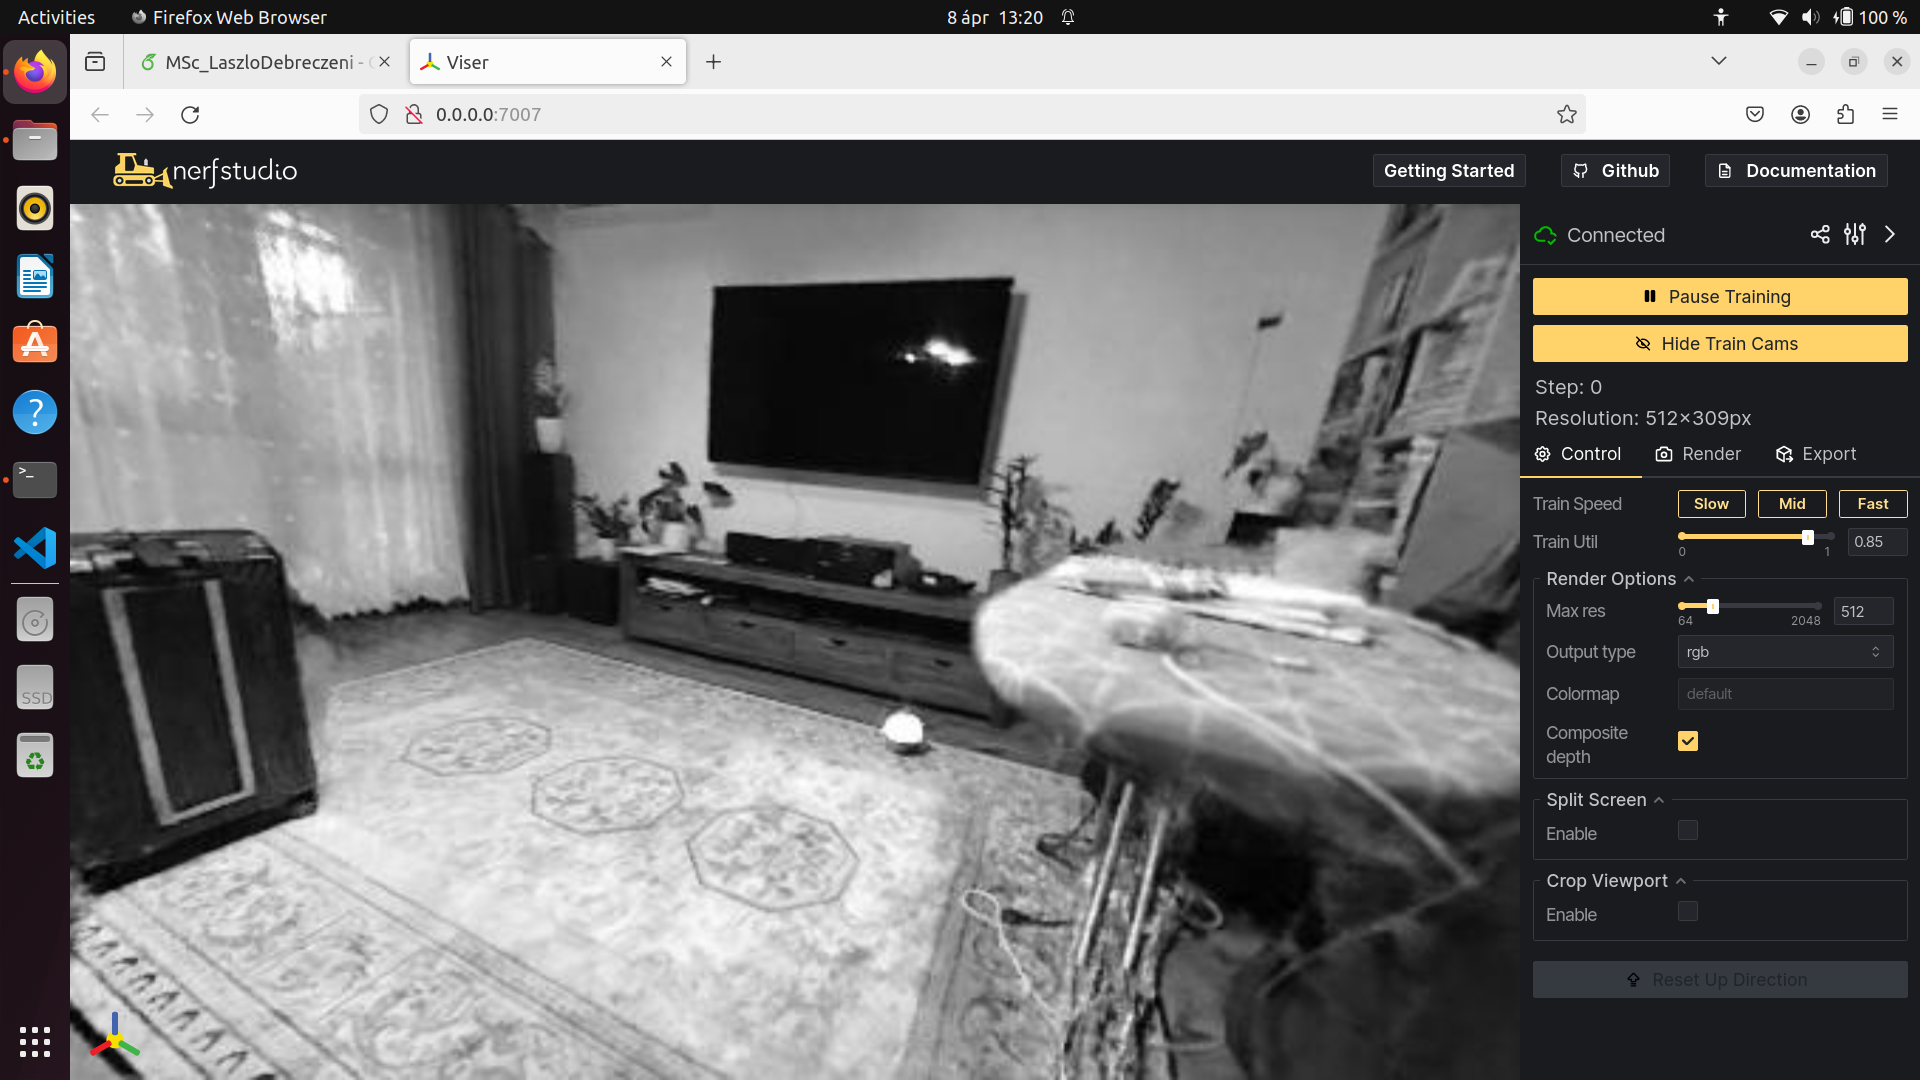
\includegraphics[width=150mm, keepaspectratio]{figures/trained_nerf_karcag1.png}
	\caption{Trained nerfacto model}
	\label{fig:trained_nerf_karcag}
\end{figure}

The result was not without concerns due to the imperfect input. I captured the video at late afternoon so the lights were on. As seen in Figure~\ref{fig:trained_nerf_karcag}, the lights reflected on the TV's screen and some more shiny surfaces causing significant perturbation in the training. The other problem was caused by the length of the camera's cable. The device uses an USB3 cable for power and data transport and thanks to this the cable is relatively short for making large scale movements around the laptop connected to it. This resulted in blurry sections in the scene because I was not able to capture every object in the room from every direction.

The nerfstudio is capable of generating point clouds from the trained model, we can specify our needs on the viewer which generates us a command that we can run. A point cloud can be seen on Figure~\ref{fig:nerfstudio_point_cloud}.

\begin{figure}[htbp]
	\centering
	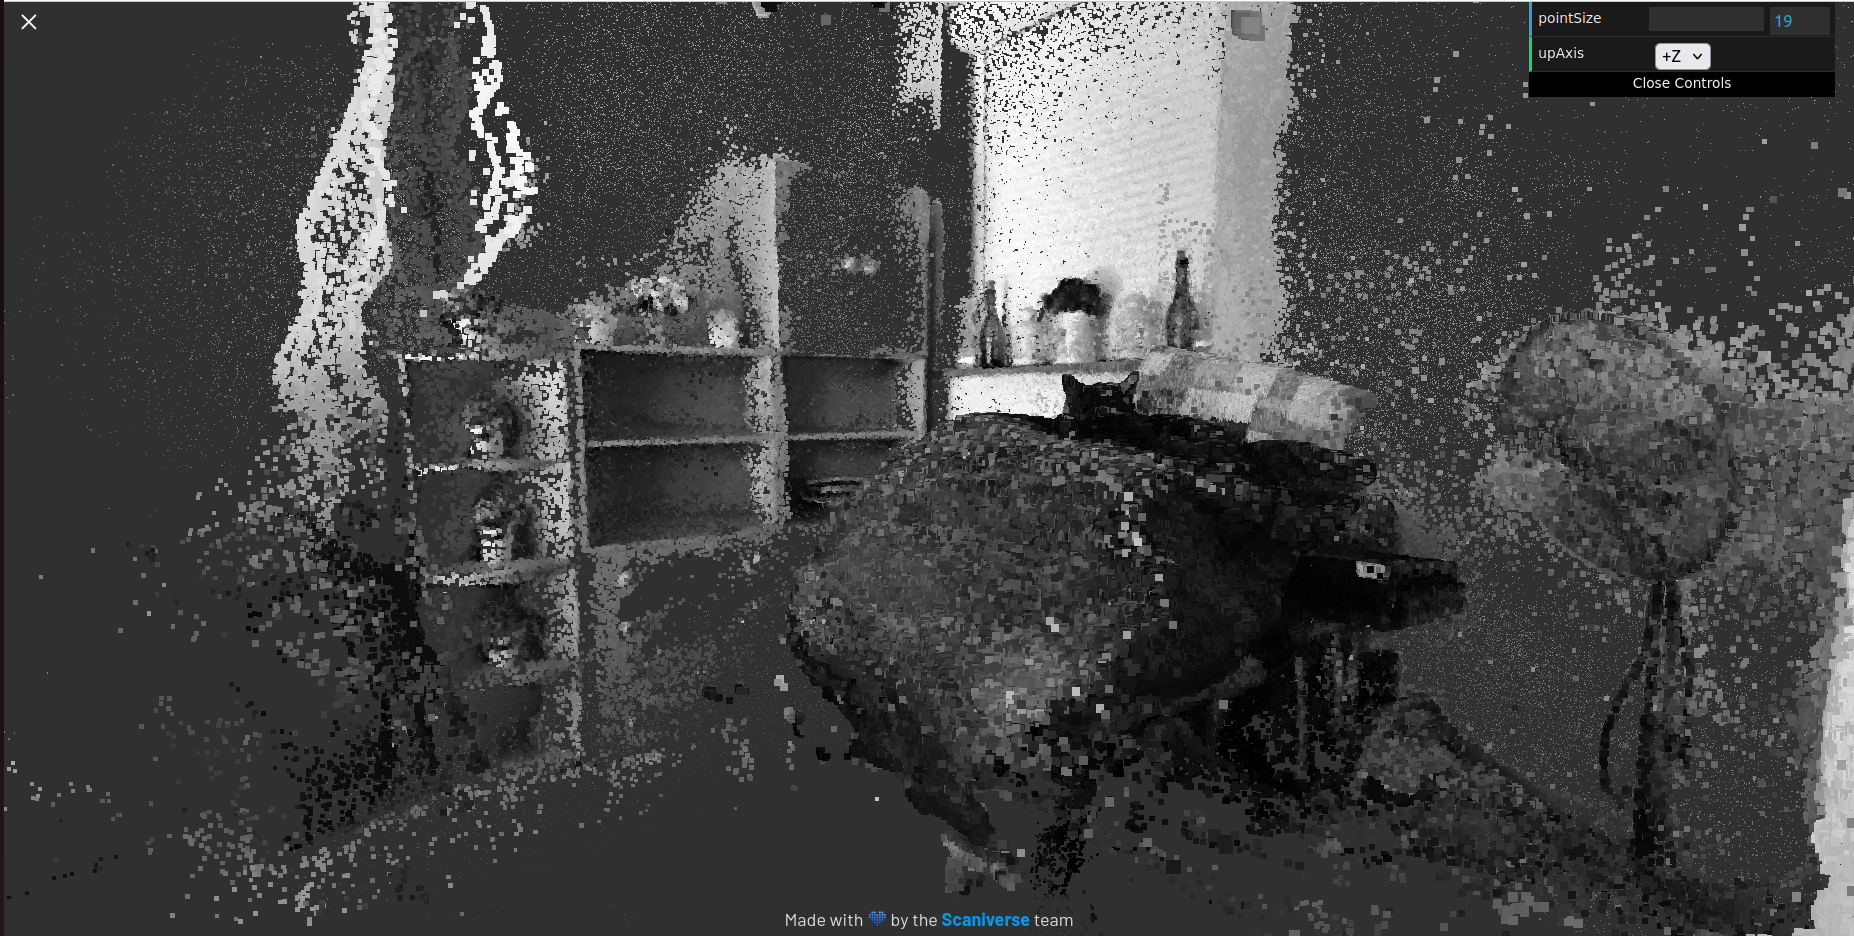
\includegraphics[width=150mm, keepaspectratio]{figures/nerfacto_point_cloud1.png}
	\caption{Point cloud from trained nerfacto model}
	\label{fig:nerfstudio_point_cloud}
\end{figure}

Overall, apart from the errors, a surprisingly good model has been created, thus proving the raison d'être of NeRFs.

\section{Experimenting with Luma AI}

Later on we tried out an interesting, more user-friendly method of training NeRFs: Luma AI's iOS application\footnote{\url{https://apps.apple.com/us/app/luma-ai/id1615849914}} (the application exists for Android, too\footnote{\url{https://play.google.com/store/apps/details?id=ai.lumalabs.polar&hl=en_US&pli=1}}). We must own a phone with a LIDAR to use the app, I tried it using an iPhone 13 Pro and it worked absolutely well under it. I captured my cat's (Szotyi's) toy as a test. First I needed to specify the object's dimensions in a modern AR view, then I had to create pictures of the toy from different angles and positions. The app uploaded the images to the cloud and after some time the NeRF was trained so we could inspect it. The results were truly breathtaking, it was as realistic as the object was right in front of us as seen on Figure~\ref{fig:luma_ai_szotyi_toy}

\begin{figure}[htbp]
	\centering
	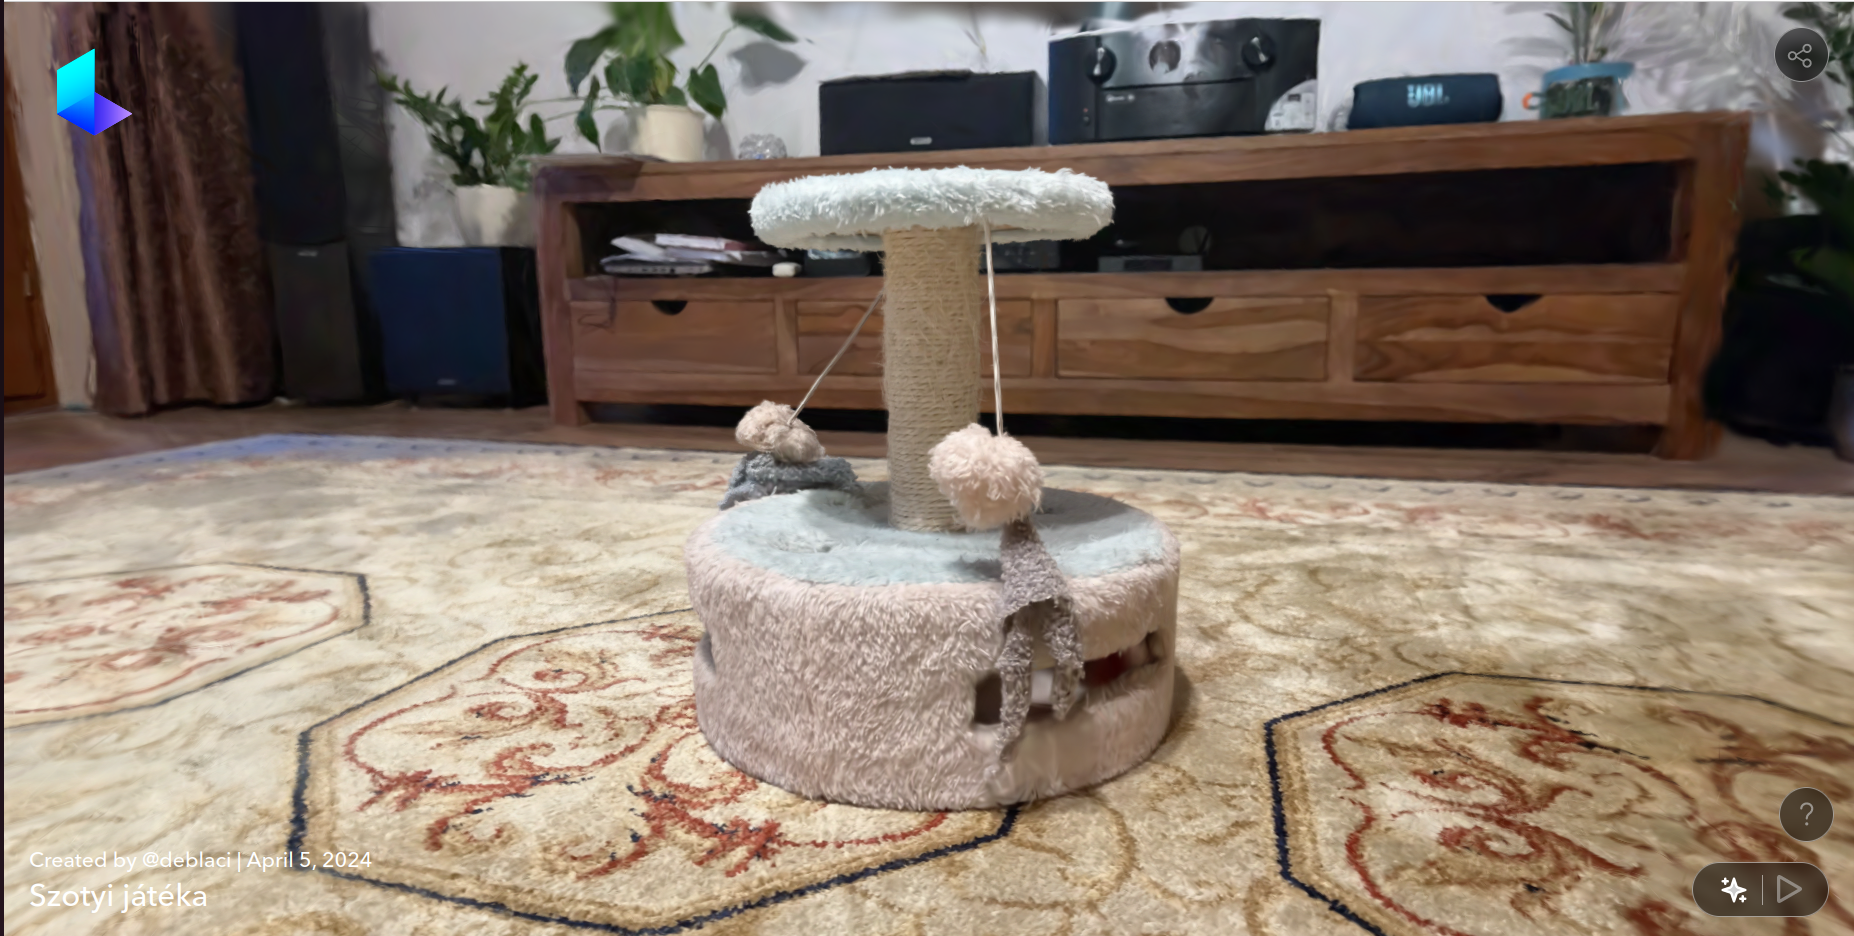
\includegraphics[width=150mm, keepaspectratio]{figures/szotyi_jateka_luma_ai.png}
	\caption{Szotyi's toy recreated by Luma AI}
	\label{fig:luma_ai_szotyi_toy}
\end{figure}

\section{Experimenting with Gaussian Splatting}

As another approach for photorealistic reconstruction we tried out some Gaussian Splatting~\cite{3DGS} implementations. I found out that nerfstudio has a model that uses Gaussian Splatting, this model is called splatfacto~\cite{splatfacto} and since I already used nerfstudio I gave it a try. Needless to say it was not without hard parts. As I used the \verb|dromni/nerfstudio| image I always got an error by CUDA because the image did not find it installed (although it was). After some hours of debugging I tried to use the \verb|nerfstudio/nerfstudio| image to see if it works or not. Well, it did not work but I got another error message for the sake of change:

\FloatBarrier
\begin{lstlisting}[language=bash,frame=single,float=!ht]
assert block width > 1 and block width <= 16, 
"block width must be between 2 and 16"
AssertionError: block width must be between 2 and 16
\end{lstlisting}

As I searched for a solution it soon became clear that this is a very low-level problem with either nerfstudio or the splatfacto model\footnote{\url{https://github.com/nerfstudio-project/gsplat/issues/159}}. I tried upgrading the \verb|gsplat| package but the issue remained.

After the failures we tried another Gaussian Splatting implementation\footnote{\url{https://github.com/graphdeco-inria/gaussian-splatting}} which finally started training but it threw \verb|CUDA out of memory| error every time. I inspected the repository and the developers stated that this works with 24 GB of VRAM. I have a GTX1660 GPU in my laptop with 6 GB of VRAM thus it was not enough for training. I tried using Google Colab for training but after it finished it had problems with saving the splats because the command always stopped with Out Of Memory errors and I was left there without the finished splat. My advisor, Gábor tried training on his GTX1080 and fortunately it had enough VRAM to finish it but the result is not worth even an image here because it was too blurry.

\chapter{Experiments in 3D mapping} \label{experiments_3d_mapping}

\section{Overview}

In this chapter, we transition to using various 3D mapping solutions for real-time mapping on the Turtlebot4, running ROS2. This involved extensive testing of RTAB-Map~\cite{RTAB_Map_docs} with the OAK-D camera and Nvidia's nvblox~\cite{nvblox_docs} to assess their effectiveness and identify any limitations, particularly in terms of speed and orientation tracking.

Since the Turtlebot4 is running ROS2, I needed to find a tool that can do the mapping and runs on the said framework. We have experimented with RTAB-Map (Real-Time Appearance-Based Mapping) and nvblox.


\section{RTAB-Map using OAK-D} \label{experiments_rtab_map}
First, I tried out RTAB-Map with the OAK-D camera. It is already implemented in ROS2 and it can be launched with the following command:
\FloatBarrier
\begin{lstlisting}[language=bash,frame=single,float=!ht]
$ ros2 launch depthai_ros_driver rtabmap.launch.py
\end{lstlisting}

The launched tool's UI can be seen on Figure \ref{fig:rtabmap_ros}. The top left panel shows the last keyframe captured by the camera, under it we can see the actual image recorded by it. On the right, we can inspect the built map:

\begin{figure}[htbp]
	\centering
	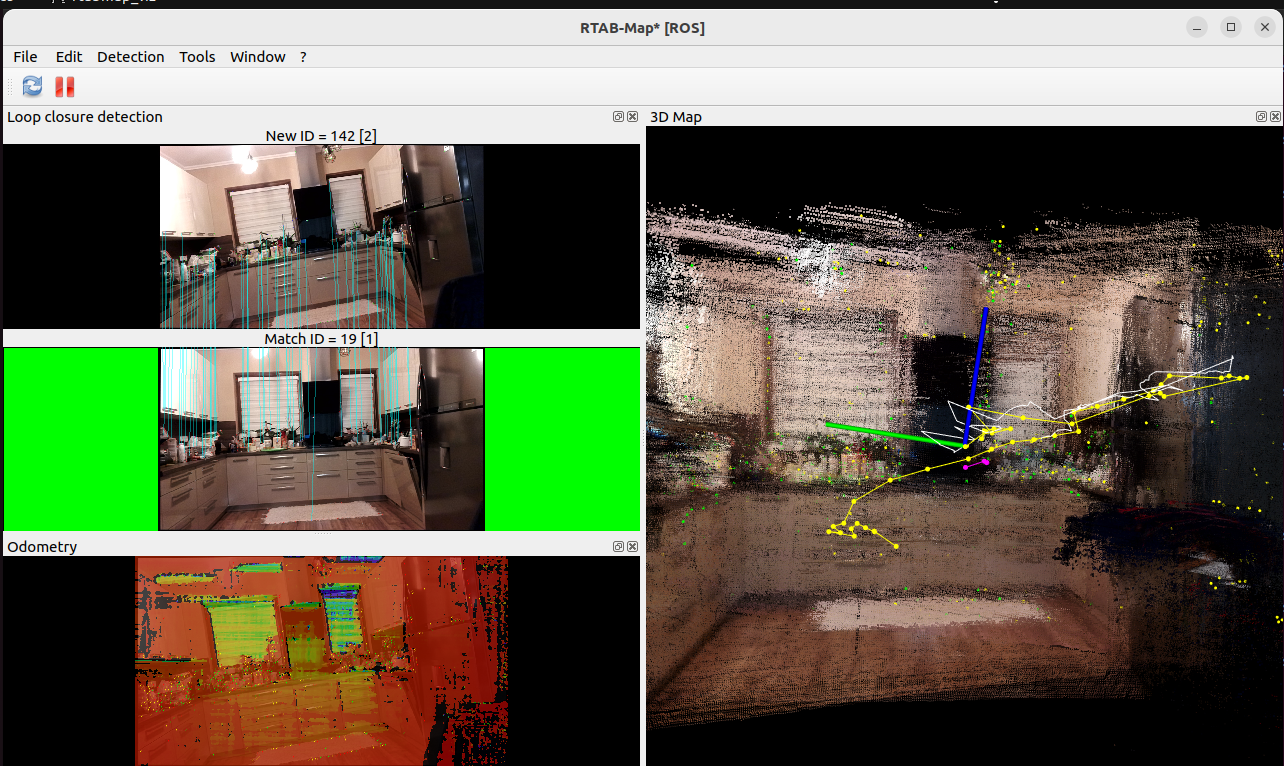
\includegraphics[width=150mm, keepaspectratio]{figures/rtabmap_ros.png}
	\caption{RTAB-Map ROS2}
	\label{fig:rtabmap_ros}
\end{figure}

When the device loses its orientation, it shows the last known position on the bottom left panel. When this happens the mapping stops and we have to navigate back to the exact same position where we lost track to get back on it and continue with the mapping. This is a huge downside of the application because this can happen quite a lot (especially in environments with poor lighting). Furthermore, we sometimes had to restart the entire mapping process because, although we returned the camera to the last known position, RTAB-Map could not recognize it. Another disadvantage of the tool is its speed; the camera's image lags significantly.

For the appropriate usage of RTAB-Map we had to modify its launch files. Our goal was to start the camera on the robot (because it is attached to it), then publish the images and IMU data onto a ROS topic which can be processed by the notebook on top.

When we start the \verb|rtabmap.launch.py| launch file inside the \verb|depthai_ros_driver| package it automatically starts the camera's node in addition to the RTAB-Map node. It was not ideal for us since the camera node should run on the robot and the RTAB-Map (which requires more computation resources) on the notebook. Our solution was to create a new launch file (which can be examined at \ref{rtabmap_custom_launch_file}) based on \verb|rtabmap.launch.py| which starts everything but the camera node. With the help of this we can launch RTAB-Map on the notebook without the camera. The camera can be started on the robot with the basic \verb|camera.launch.py| launch file from the \verb|depthai_ros_driver| package. A mapping made with this approach can be seen on Figure~\ref{fig:rtabmap_nokia}.

To summarize our experiments, due to the lag and loss of orientation, it was problematic to create a map even in a small room (seen on Figure~\ref{fig:rtabmap_nokia}, it can be seen that a lot of irrelevant points are added to the map). This issue is more severe on the actual robot, which can turn at high angular speeds. It always lost track, and navigating back to the last known position was time-consuming and only moderately successful.

\begin{figure}[H]
	\centering
	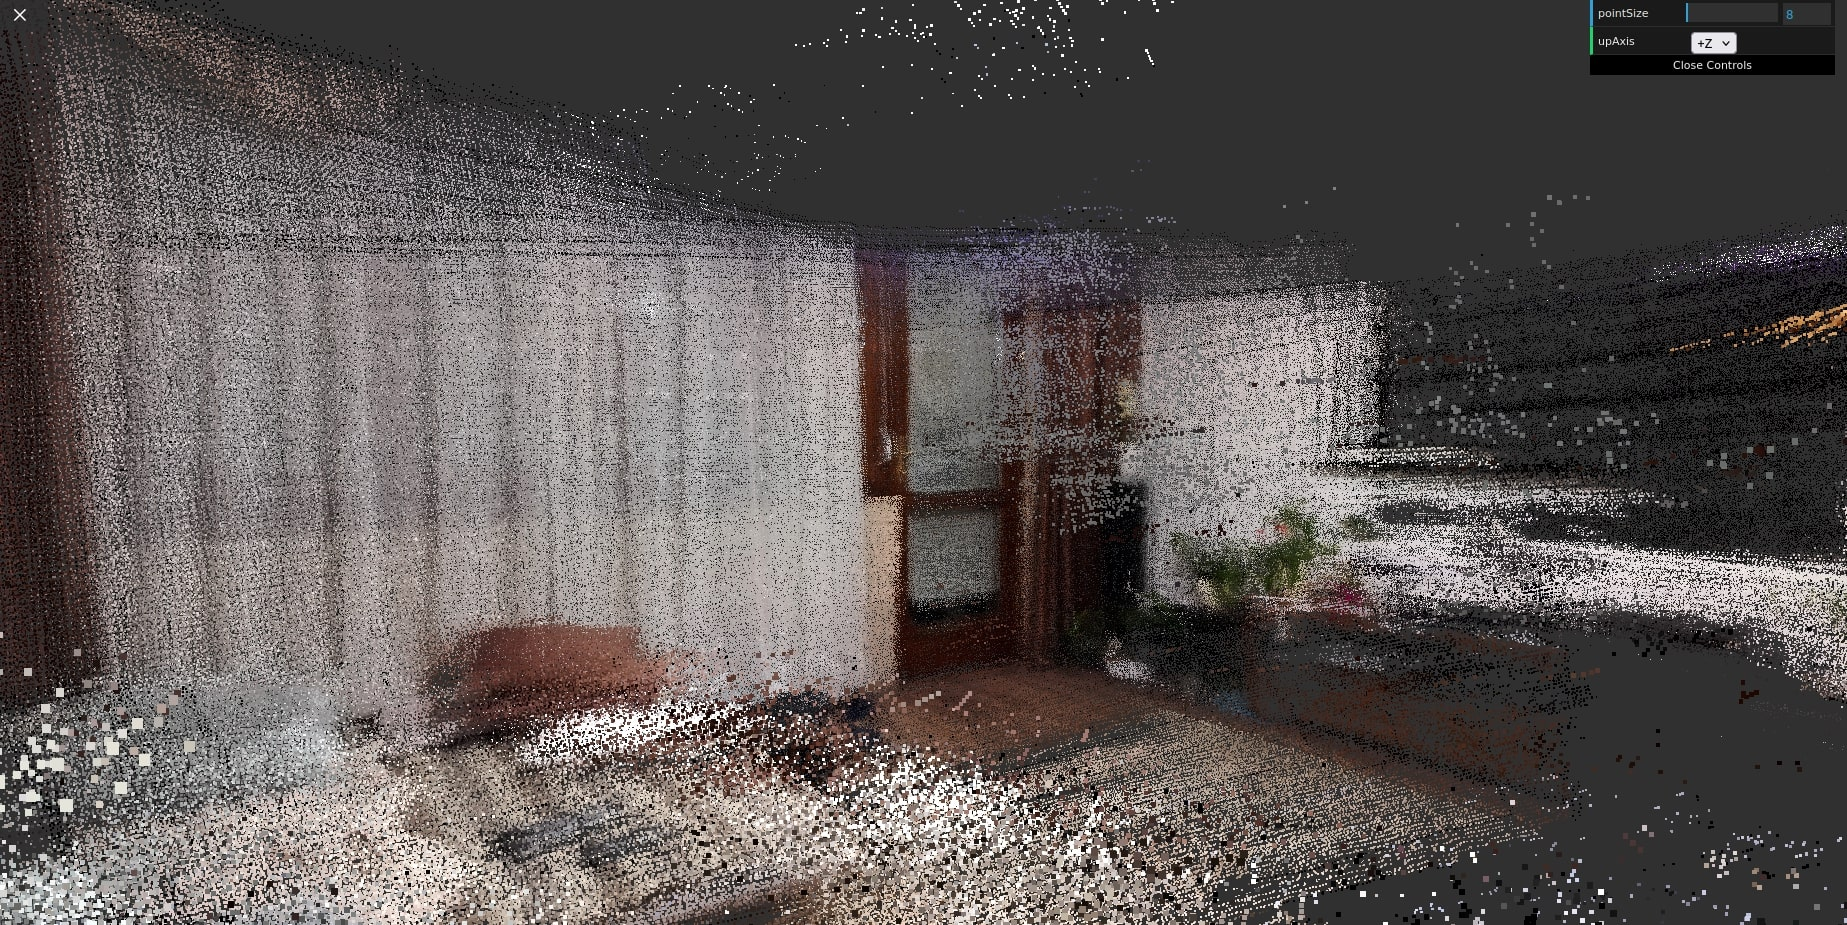
\includegraphics[width=150mm, keepaspectratio]{figures/rtabmap_ros_home.png}
	\caption{RTAB-Map ROS generated point cloud map of our living room, camera held by hand}
	\label{fig:rtabmap_nokia}
\end{figure}

\FloatBarrier
\section{RTAB-Map iOS}

We tried the iOS version of RTAB-Map as a matter of interest and it worked more effectively than the ROS version with the OAK-D camera. I used the same iPhone 13 Pro and I got a relatively good reconstruction of my apartment, as shown on Figure~\ref{fig:luma_ai_szotyi_toy}. This app can create a mesh or a photorealistic map of our surrounding. When I generated a map it was running much smoother than the ROS version: it was not lagging at all and did not lost track even in rooms with poor light. A generated mesh map can be seen on Figure~\ref{fig:rtabmap_ios}.

\begin{figure}[htbp]
	\centering
	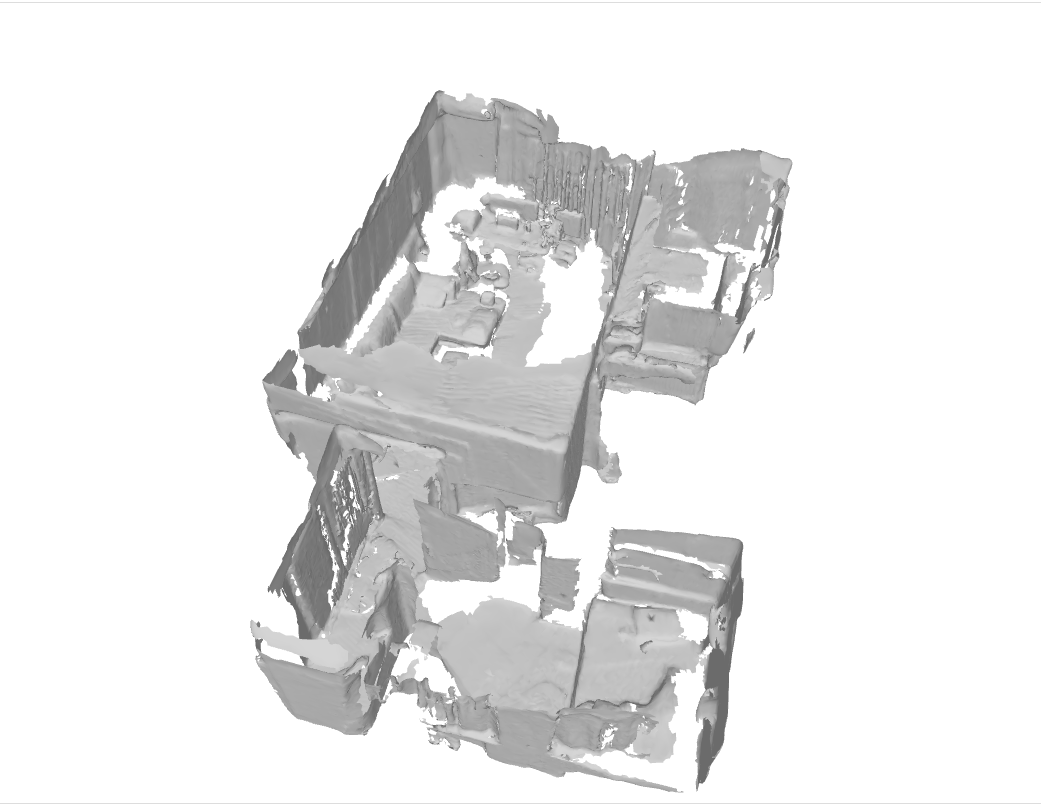
\includegraphics[width=150mm, keepaspectratio]{figures/rtabmap_ios.png}
	\caption{RTAB-Map iOS generated mesh map}
	\label{fig:rtabmap_ios}
\end{figure}

The holes in the floor are visible because the dark brown laminate reflected the light coming through the window. This made the area that RTAB-Map did not recognize due to the diversity of colors.

\section{Nvblox}

NVIDIA’s nvblox is a GPU-accelerated spatial mapping library designed to work seamlessly with ROS2 and other robotics frameworks for real-time 3D environment reconstruction. Leveraging NVIDIA’s CUDA technology, nvblox processes data from depth sensors and LIDAR in real time, enabling robots to build and update dense 3D maps of their surroundings with low latency. Its main use cases include robotics applications requiring immediate spatial awareness, such as autonomous navigation, manipulation, and exploration in dynamically changing environments.

One of the key advantages of nvblox is its ability to generate high-resolution voxel grids and mesh representations at impressive speeds, a performance largely unattainable with CPU-only mapping solutions. nvblox achieves this by maintaining and updating a voxel grid map where each voxel represents a small cube in the 3D environment, storing spatial information like occupancy and color. It also incorporates functionality to convert voxel maps into triangular meshes, which can then be visualized or further processed. With its ROS2 compatibility, nvblox can work as a ROS node, allowing direct integration with popular robotic systems and sensor data sources like RGB-D cameras, stereo cameras, and LIDAR, making it a practical solution for ROS-based projects.

Another significant feature of nvblox is its flexibility to run on various NVIDIA platforms, including Jetson devices, which are popular in edge computing and mobile robotics. This makes nvblox ideal for field applications where high-performance spatial understanding is critical. By reducing the computational load traditionally associated with real-time 3D mapping and enhancing efficiency, nvblox enables the creation of robust, high-fidelity maps that allow robots to react to and understand their environments effectively.

To begin using nvblox, I installed its dependencies and started the provided Docker container. However, when attempting to run the example code, I encountered frequent crashes. This was due to nvblox’s requirement for a minimum of 8 GB of VRAM, while my notebook, equipped with a GTX 1660 Ti GPU, only has 6 GB. Occasionally, the example did run successfully, as shown in Figure~\ref{fig:nvblox_example}. In this figure, you can observe how nvblox generates a voxel map by combining data from color and depth images along with LIDAR inputs, producing a comprehensive spatial map.

\begin{figure}[htbp]
	\centering
	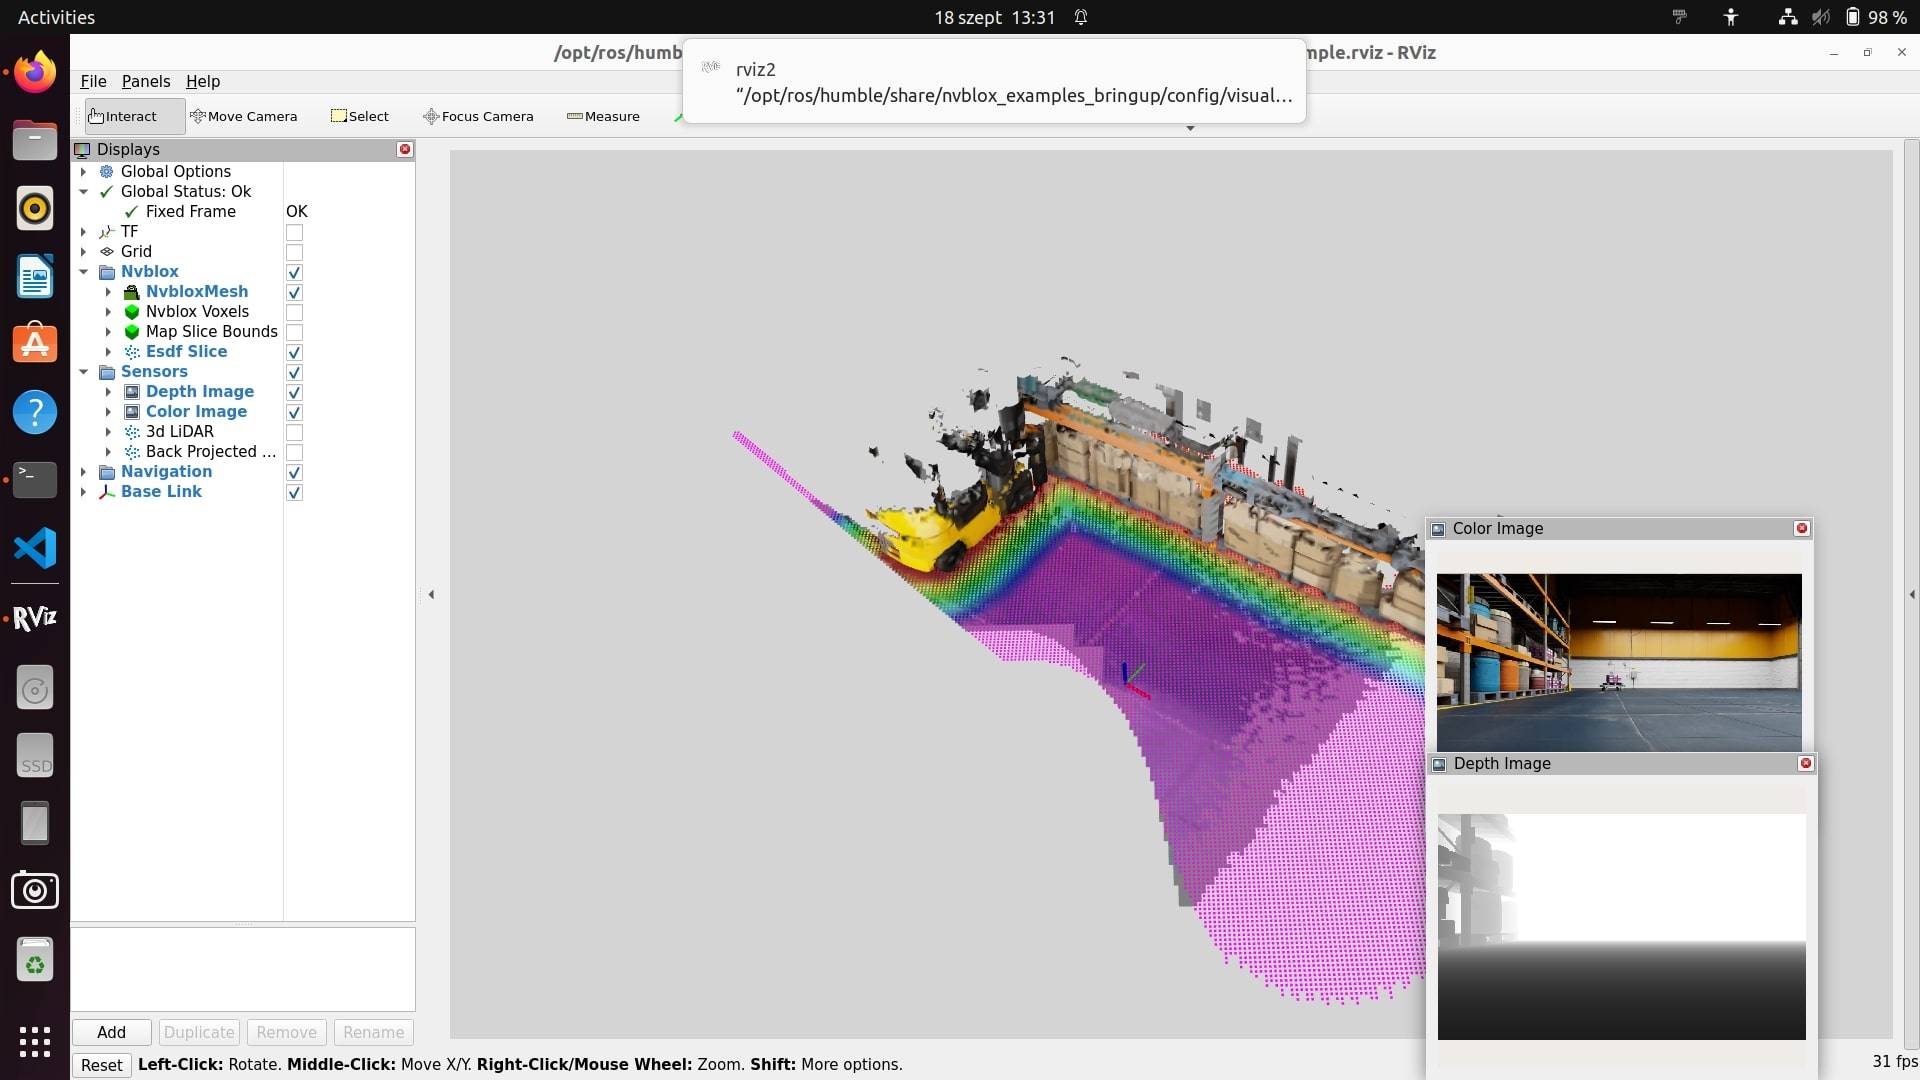
\includegraphics[width=150mm, keepaspectratio]{figures/nvblox.png}
	\caption{Running nvblox example}
	\label{fig:nvblox_example}
\end{figure}

Following my experiments with nvblox, I explored NVIDIA's Isaac VSLAM, an advanced SLAM tool that leverages NVIDIA GPUs to perform stereo visual inertial odometry (SVIO). We anticipated that Isaac VSLAM would be beneficial because it aligns well with the capabilities of the OAK-D cameras, which also support SVIO. Isaac VSLAM outputs data that can be combined with wheel odometry and LIDAR inputs, producing highly accurate localization data for ROS2's Nav2 navigation framework. Figure~\ref{fig:isaac_vslam_example} shows the Isaac VSLAM example in action. To test the Isaac VSLAM module, I used NVIDIA's isaac-sim Omniverse simulator \cite{isaac_sim_docs}. Unfortunately, the simulation environment failed to render visuals because Omniverse requires an RTX GPU to handle its advanced rendering features, which my GTX GPU could not support.

\begin{figure}[htbp]
	\centering
	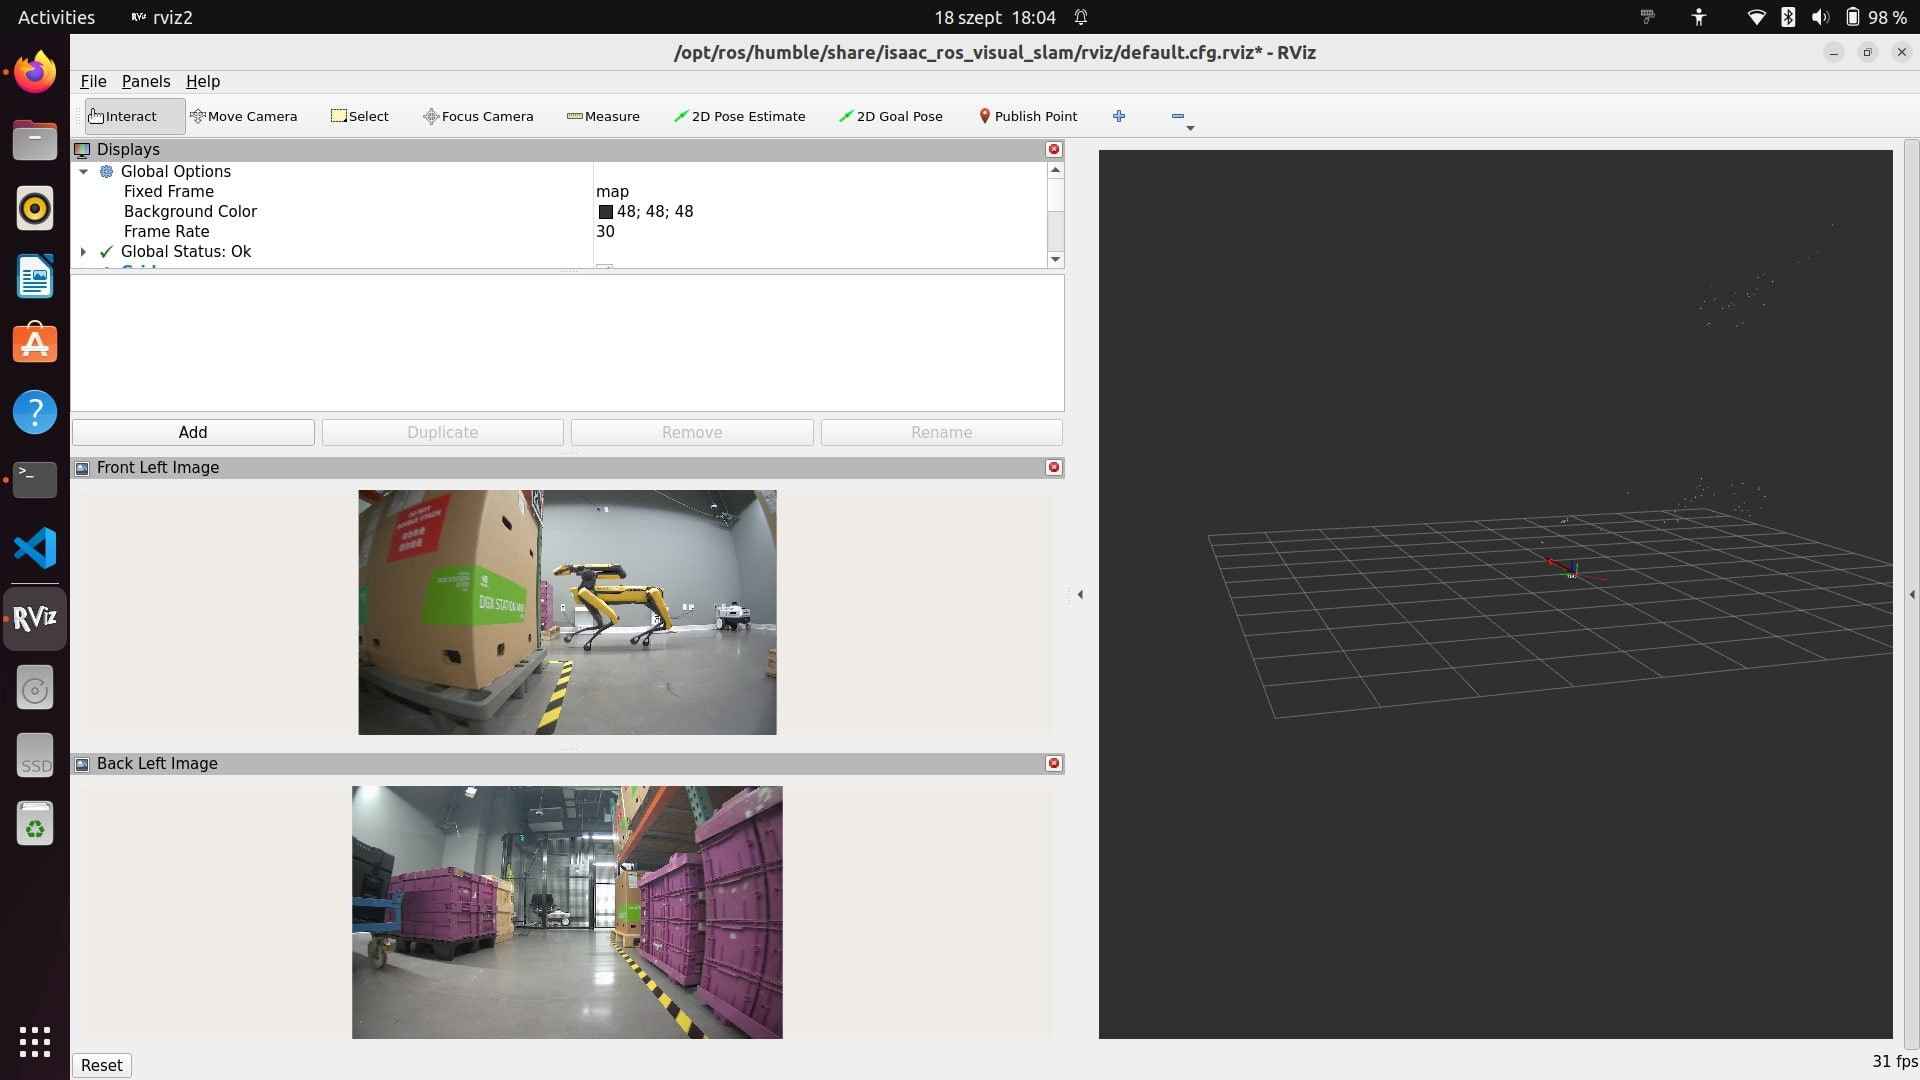
\includegraphics[width=150mm, keepaspectratio]{figures/isaac_vslam_example.png}
	\caption{Running Isaac VSLAM example}
	\label{fig:isaac_vslam_example}
\end{figure}

In the end, we opted not to use NVIDIA Isaac on the Turtlebot4 robot due to its GPU-intensive algorithms, which require at least an 8 GB VRAM-equipped Jetson module. Our robot was equipped with a Raspberry Pi 4, and we decided against investing in a Jetson due to the additional cost, which we deemed impractical for this project.

\chapter{Implementation} \label{implementation}

\section{RTAB-Map}

For the appropriate usage of RTAB-Map~\cite{RTAB_Map_docs} we had to modify its launch files. Our goal was to start the camera on the robot (because it is attached to it), then publish the images and IMU data onto a ROS topic which can be processed by the notebook on top.

When we start the \verb|rtabmap.launch.py| launch file inside the \verb|depthai_ros_driver| package it automatically starts the camera's node in addition to the RTAB-Map node. It was not ideal for us since the camera node should run on the robot and the RTAB-Map (which requires more computation resources) on the notebook. Our solution was to create a new launch file (which can be examined at \ref{rtabmap_custom_launch_file}) based on \verb|rtabmap.launch.py| which starts everything but the camera node. With the help of this we can launch RTAB-Map on the notebook without the camera. The camera can be started on the robot with the basic \verb|camera.launch.py| launch file from the \verb|depthai_ros_driver| package. A mapping made with this approach can be seen on Figure~\ref{fig:rtabmap_nokia}.

\section{Person detection}

For the person detection we first tried out the Spectacular AI's example on the robot's camera but we soon realised that the position of it is not ideal for detecting objects. Due to the platform above the robot it limits the FOV (Field of View) of the camera so much that if we stood 2-3 meters away from the robot only our legs were visible thus the detection was not working. Our solution for this problem was to put the camera right at the front of the platform with some plasticine and it worked because the FOV increased a lot. The detection of my advisor with the camera at front can be seen on Figure \ref{fig:person_detection_camera_at_front_nokia} (the other detected person is a woman on a poster).

\begin{figure}[htbp]
    \centering
    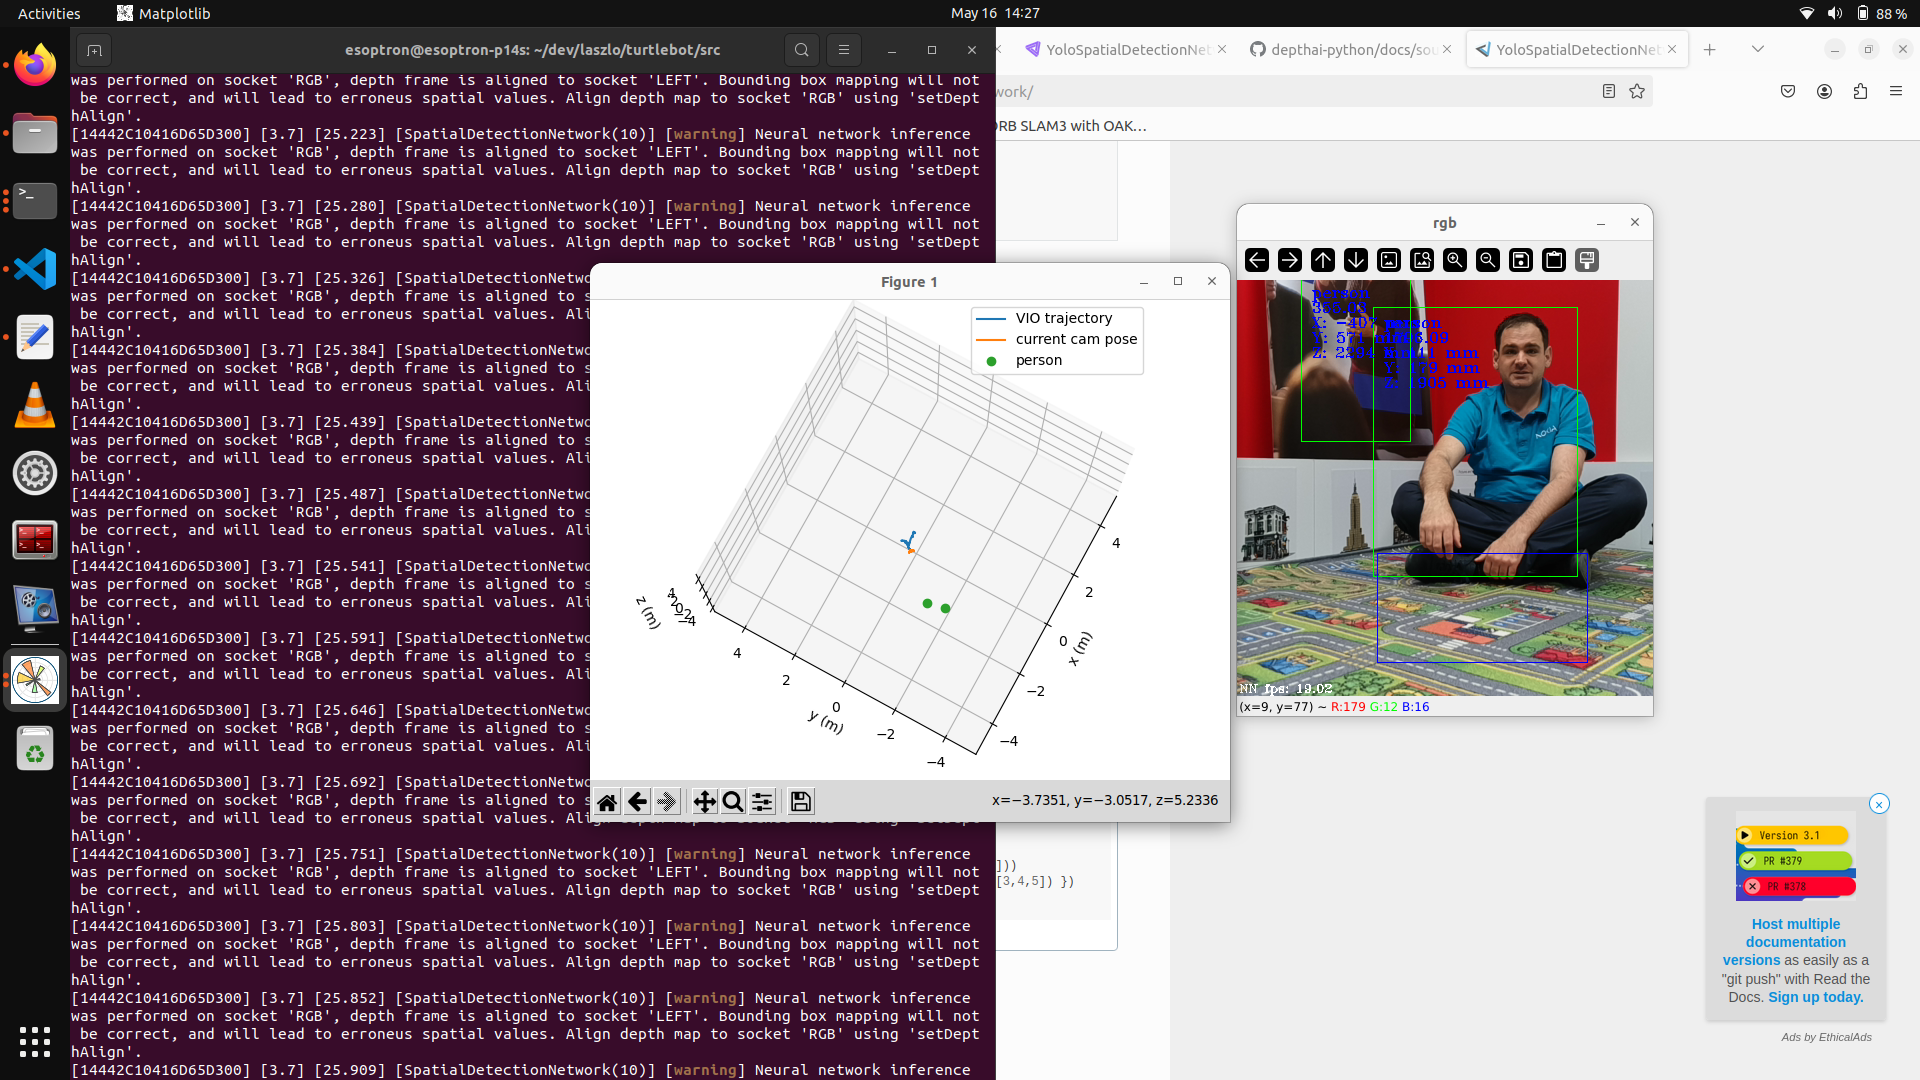
\includegraphics[width=150mm, keepaspectratio]{figures/person_detection_camera_at_front_nokia.png}
    \caption{Person detection with the camera at front at Nokia Bell Labs}
    \label{fig:person_detection_camera_at_front_nokia}
\end{figure}

After we experimented with the FOV and the example detection script I created a custom script based on the example which uses the camera to detect persons and publish their location in world coordinates on a ROS topic (the code can be examined at \ref{custom_person_detector}). It is worth mentioning that the base example (and my code too) is needed to be upgraded because after some detections it freezes with an error indicating that the IMU buffer size is exceeded. It may be because the IMU sends data too rapidly and the configuration of the \verb|SpatialLocationCalculator| node uses a buffer that is too small. Unfortunately we had no time to further investigate this issue but it seems really complex due to it lays inside the \verb|SpatialLocationCalculator| camera pipeline node.

\chapter{Evaluation} \label{evaluation}

\section{Overview}
This chapter evaluates the photorealistic scene reconstruction pipeline. The pipeline is divided into two primary stages: post-processing keyframe images and generating a Gaussian splat model. For testing the post-processing script, I created a scene with challenging conditions, including high angular speeds and overexposure, to evaluate the script's ability to filter out unsuitable images. A separate scene with an old microscope was used to test the Gaussian splatting and assess the 3D reconstruction quality. 

\section{Post-Processing Script Evaluation}
To assess the effectiveness of the post-processing script, I created a dataset with simulated challenging conditions by making rapid movements and positioning a flashlight near the camera. These actions mimicked high angular speeds and overexposure, aiming to introduce blurry and overexposed frames into the dataset. Figure~\ref{fig:keyframes_before_process} shows the saved keyframe images before running the script.

\FloatBarrier
\begin{figure}[htbp]
	\centering
	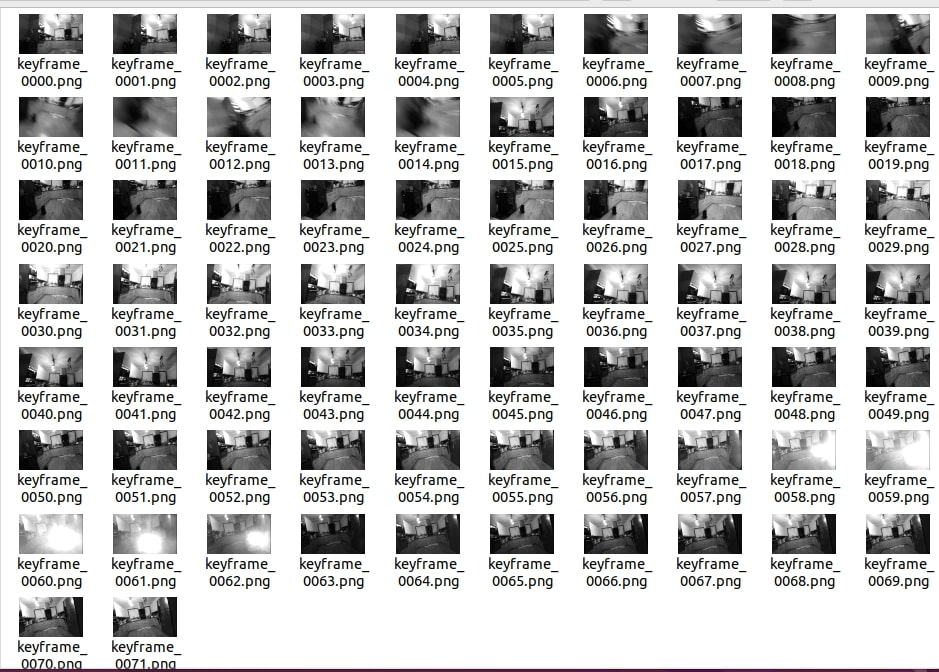
\includegraphics[width=150mm, keepaspectratio]{figures/keyframes_before_process.png}
	\caption{Saved images from mapping by the \textit{keyframe\_saver} node before processing}
	\label{fig:keyframes_before_process}
\end{figure}
\FloatBarrier

After running the script, which detected and removed blurry or overexposed frames, the processed image set can be seen in Figure~\ref{fig:keyframes_after_process}. The script’s output, detailing deletions and renamings, is shown in Figure~\ref{fig:image_process_script_output}. Examples of detected blurry and overexposed images that the script correctly flagged for deletion are displayed in Figure~\ref{fig:blurry_overexposed_example}.

\FloatBarrier
\begin{figure}[htbp]
	\centering
	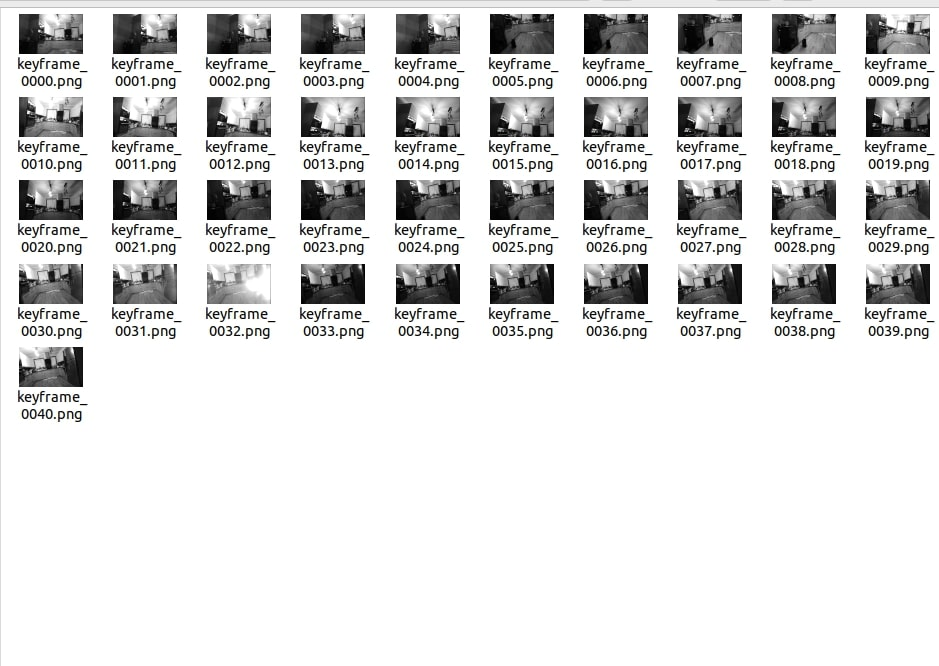
\includegraphics[width=150mm, keepaspectratio]{figures/keyframes_after_process.png}
	\caption{Remaining images after running the post-processing script}
	\label{fig:keyframes_after_process}
\end{figure}

\begin{figure}[htbp]
	\centering
	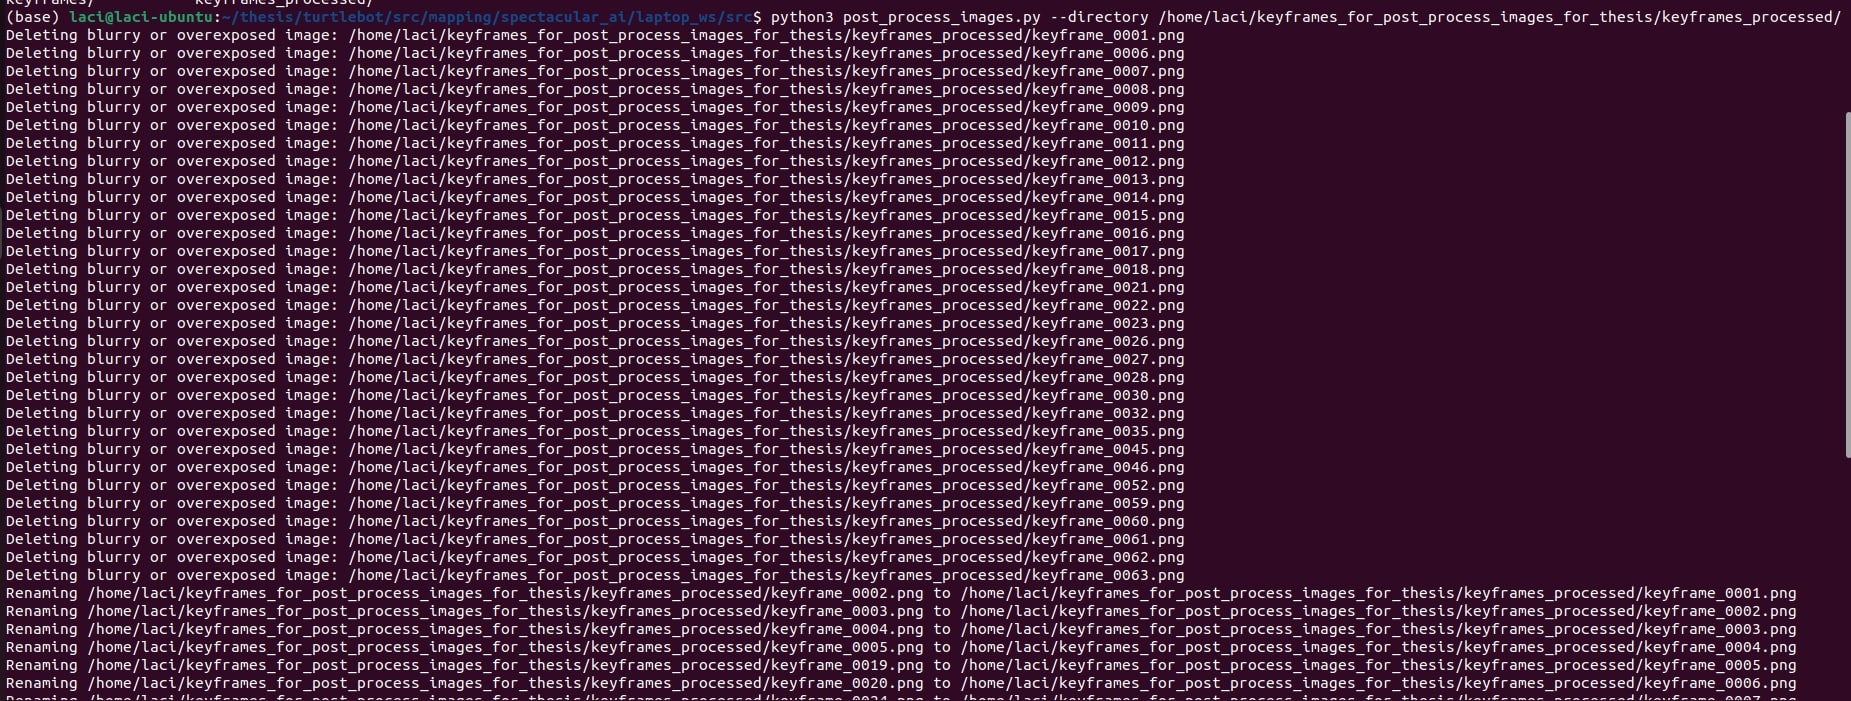
\includegraphics[width=150mm, keepaspectratio]{figures/process_script_output.png}
	\caption{Terminal output of the post-processing script}
	\label{fig:image_process_script_output}
\end{figure}


\begin{figure}[htbp]
	\centering
	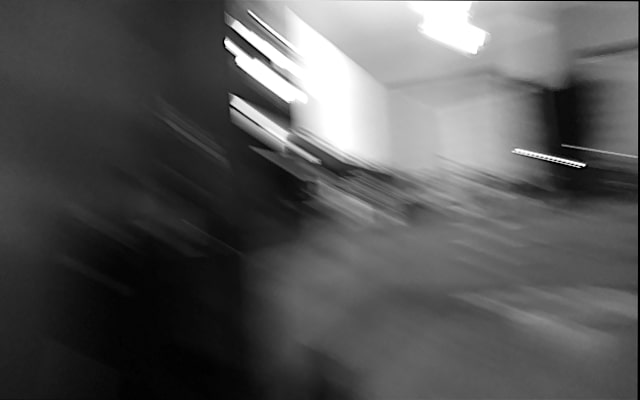
\includegraphics[width=67mm, keepaspectratio]{figures/example_for_blurry.png}\hspace{1cm}
	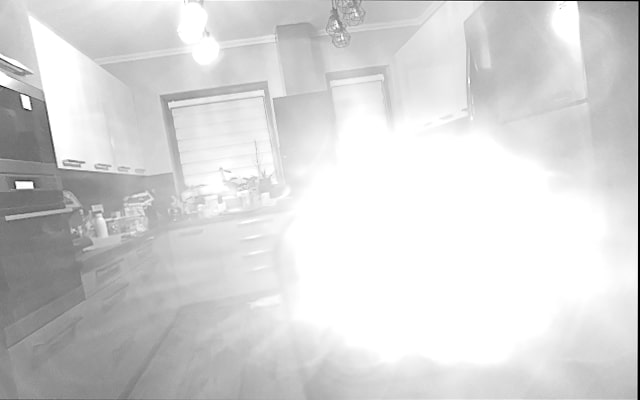
\includegraphics[width=67mm, keepaspectratio]{figures/example_for_overexposed.png}\\\vspace{5mm}
	\caption{Examples of blurry (left) and overexposed (right) images successfully detected and deleted by the script}
	\label{fig:blurry_overexposed_example}
\end{figure}
\FloatBarrier

\section{Gaussian Splatting Evaluation}
To evaluate the Gaussian splatting capabilities, I recorded a scene with an old microscope, positioned centrally in a controlled setting. After running the post-processing script to filter the images, I trained the \verb|splatfacto-big| model on the processed dataset. Figure~\ref{fig:spai_gsplat} displays the reconstructed splat.

\begin{figure}[htbp]
	\centering
	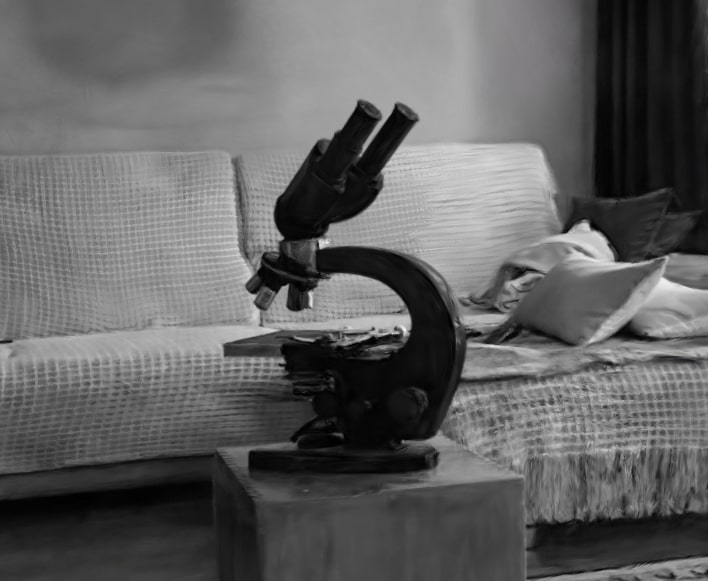
\includegraphics[width=150mm, keepaspectratio]{figures/spai_gsplat.png}
	\caption{Reconstructed microscope scene using Gaussian splatting}
	\label{fig:spai_gsplat}
\end{figure}

The reconstructed item appears slightly blurry, with some dark areas within the image. This effect results from the high amount of incoming light through windows positioned to the right of the capture area, which introduces lighting variations and subtle perturbations to the Gaussian splatting process. Additionally, the generated splat is in grayscale, as the mapping node uses the Spectacular AI Python SDK's camera pipeline. This SDK exclusively utilizes grayscale stereo cameras, omitting the RGB camera. Unfortunately, the pipeline configuration is fixed, so activating the RGB camera was not an option. However, given the spatial calculation speed and accuracy provided by this SDK, we chose to prioritize these qualities over color data. Implementing a custom spatial camera pipeline to support RGB capture was evaluated but ultimately deemed too time-intensive for our timeline.

Overall, this pipeline enables high-quality, photorealistic reconstructions, even without RGB data. Despite the grayscale limitation, the combination of Gaussian splatting and the Spectacular AI SDK’s stereo-based spatial accuracy produces detailed and realistic 3D models. The pipeline captures fine spatial features and preserves depth and texture fidelity, creating a solid foundation for effective reconstructions in real-world settings.

\chapter{Summary} \label{summary}

The goal of this thesis was to implement an environment mapping system on a mobile robot equipped with a stereo camera at Nokia Bell Labs Budapest. Additionally, the robot was intended to detect and interact with people by either following or avoiding them. Another objective was to establish a pipeline for generating photorealistic reconstructions of the mapped environment.

In the first semester of my Master of Science thesis, I became familiar with the Turtlebot4 mobile robot and its OAK-D stereo camera. I conducted experiments with the camera, the Spectacular AI SDK, photorealistic reconstructions, mapping, and object detection.

The Turtlebot4 offered considerable potential due to its advanced hardware: a Raspberry Pi 4 controller running Ubuntu 22.04 with ROS2 compatibility, and the OAK-D Pro stereo camera. The camera's capabilities included generating depth maps using its stereo lenses and accurately determining object positions using its Visual Processing Unit (VPU). Furthermore, with its Inertial Measurement Unit (IMU), the robot's poses could be calculated in real-time. Leveraging the Spectacular AI SDK, I explored its examples, which demonstrated the SDK's value for mapping and object detection tasks.

Photorealistic scene reconstruction is gaining traction, and as an additional goal, we sought to achieve reconstructions solely using data recorded during mapping. In the first semester, I tested NeRFs and Gaussian Splatting with a handheld OAK-D camera, yielding promising results that motivated further exploration in the second semester.

I initially experimented with RTAB-Map for mapping due to its support for OAK-D cameras. Unfortunately, it proved unreliable, introducing lags that hindered practical use. Interestingly, RTAB-Map's iOS application performed smoothly on my phone. Separately, I implemented a ROS2 node for person detection, which published detected individuals' coordinates. This feature leveraged the camera's VPU to run neural networks for real-time object detection. However, a critical issue arose: once a person was detected, the IMU buffer overflowed, freezing the system. Even Luxonis’ original object detection example code encountered the same problem, indicating a firmware-level issue. Consequently, I could not achieve robust person detection on the robot.

In the second semester, I explored NVIDIA's \verb|nvblox| and \verb|isaac-vslam| for mapping, implemented a custom mapping node using the Spectacular AI SDK, and developed a pipeline for creating photorealistic reconstructions.

Since RTAB-Map was unsuitable, I turned to \verb|nvblox|, a GPU-accelerated tool for voxel-based mapping compatible with the robot's camera. However, hardware limitations prevented full functionality; my GTX 1660 Ti GPU lacked the required 8 GB of VRAM, offering only 6 GB. I then explored \verb|isaac-vslam|, another NVIDIA tool for Visual SLAM that uses GPU acceleration. Its simulations can run in NVIDIA Omniverse, which supports creating diverse environments. Unfortunately, Omniverse requires an RTX GPU for hardware-accelerated ray tracing, which my GTX GPU could not provide. Ultimately, deploying \verb|nvblox| or \verb|isaac-vslam| on the robot would require a Jetson with at least 8 GB of VRAM, but budget constraints precluded this option.

In the final phase of my thesis, I developed a ROS2 mapping node using the Spectacular AI SDK to compute the robot's poses and publish its environment as a point cloud. Additional nodes, running on a notebook, collected poses, images, and point clouds at keyframes. After mapping, my post-processing script removed blurry and overexposed images and their associated poses. Another script prepared the input data for Gaussian splatting by transforming robot poses and the point cloud into the required coordinate system and embedding camera intrinsics into a JSON file describing keyframe transformations. Using this dataset, I trained a Gaussian splatting model and generated splats. However, due to noise and misalignments in the point cloud, the results did not match our expectations for photorealistic reconstruction. To prove that this approach could be used well in environment mapping I used COLMAP to predict the poses of the keyframes and a point cloud merely from images. With this approach I could achieve realistic results from the environment.

In the future, if the camera's manufacturer could solve the issues experienced in object detection, it would be possible to add a person detection feature to my mapping node. Another improvement would be a filtering and adjusting feature for the point cloud with which we would be able to create lifelike scenes from the mapped environment.

\chapter{Acknowledgement} \label{acknowledgements}

I would like to thank and give my best regards to my supervisors, Gábor Sörös and Judit Tevesz for their valuable insights throughout the development of this thesis. Their encouragement and expert advice have been invaluable in overcoming challenges and achieving my goals.

I wish to thank Nokia Bell Labs for providing me the opportunity to work on their mobile robot and for lending me an OAK-D camera with which I could experiment and implement my features at home.

My sincere thanks also go to the Spectacular AI Team, particularly Jerry Ylilammi for generously providing access to their SDK for the Raspberry Pi 4 for educational purposes. Their support allowed me to explore advanced technologies and implement key components of this project.


%%----------------------------------------------------------------------------
\chapter{\LaTeX-eszközök}
\label{sec:LatexTools}
%----------------------------------------------------------------------------
\section{A szerkesztéshez használatos eszközök}
%----------------------------------------------------------------------------
Ez a sablon TeXstudio 2.8.8 szerkesztővel készült. A TeXstudio egy platformfüggetlen, Windows, Linux és Mac OS alatt is elérhető \LaTeX-szerkesztőprogram számtalan hasznos szolgáltatással (\refstruc{fig:TeXstudio}). A szoftver ingyenesen letölthető\footnote{A TeXstudio hivatalos oldala: \url{http://texstudio.sourceforge.net/}}.

\begin{figure}[!ht]
\centering
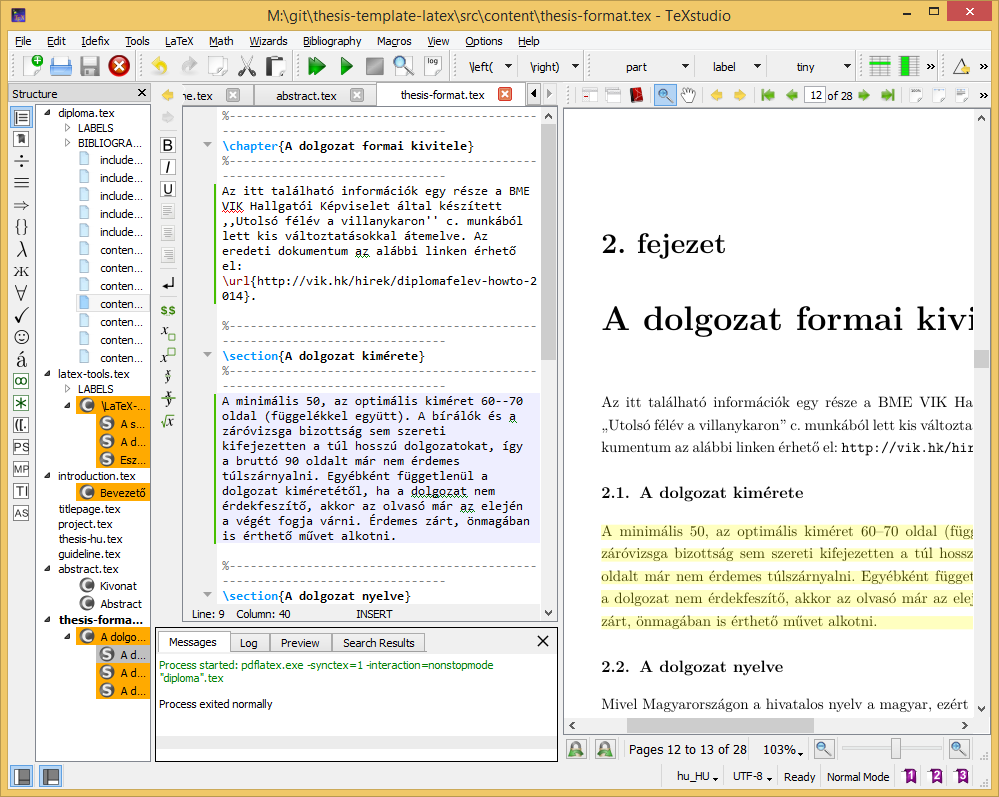
\includegraphics[width=150mm, keepaspectratio]{figures/TeXstudio.png}
\caption{A TeXstudio \LaTeX-szerkesztő.}
\label{fig:TeXstudio}
\end{figure}

A TeXstudio telepítése után érdemes még letölteni a magyar nyelvű helyesírásellenőrző-szótárakat hozzá. A TeXstudio az OpenOffice-hoz használatos formátumot tudja kezelni. A TeXstudio beállításainál a \verb+General+ fülön a \verb+Dictionaries+ résznél tudjuk megadni, hogy melyik szótárat használja.

Egy másik használható Windows alapú szerkesztőprogram a LEd\footnote{A LEd hivatalos oldala: \url{http://www.latexeditor.org/}} (LaTeX Editor), a TeXstudio azonban stabilabb, gyorsabb, és jobban használható.

%----------------------------------------------------------------------------
\section{A dokumentum lefordítása Windows alatt}
%----------------------------------------------------------------------------
A TeXstudio és a LEd kizárólag szerkesztőprogram (bár az utóbbiban DVI-nézegető is van), így a dokumentum fordításához szükséges eszközöket nem tartalmazza. Windows alatt alapvetően két lehetőség közül érdemes választani: MiKTeX (\url{http://miktex.org/}) és TeX Live (\url{http://www.tug.org/texlive/}) programcsomag. Az utóbbi működik Mac OS X, GNU/Linux alatt és Unix-származékokon is. A MiKTeX egy alapcsomag telepítése után mindig letölti a használt funkciókhoz szükséges, de lokálisan hiányzó \TeX-csomagokat, míg a TeX Live DVD ISO verzóban férhető hozzá. Ez a dokumentum TeX Live 2008 programcsomag segítségével fordult, amelynek DVD ISO verziója a megadott oldalról letölthető. A sablon lefordításához a disztribúcióban szereplő \verb+magyar.ldf+ fájlt a \verb+http://www.math.bme.hu/latex/+ változatra kell cserélni, vagy az utóbbi változatot be kell másolni a projekt-könyvtárba (ahogy ezt meg is tettük a sablonban) különben anomáliák tapasztalhatók a dokumentumban (pl. az ábra- és táblázat-aláírások formátuma nem a beállított lesz, vagy bizonyos oldalakon megjelenik alapértelmezésben egy fejléc). A TeX Live 2008-at még nem kell külön telepíteni a gépre, elegendő DVD-ről (vagy az ISO fájlból közvetlenül, pl. DaemonTools-szal) használni.

Ha a MiKTeX csomagot használjuk, akkor parancssorból a következő módon tudjuk újrafordítani a teljes dokumentumot:

\begin{lstlisting}[language=bash,frame=single,float=!ht]
$ texify -p thesis.tex
\end{lstlisting}

A \verb+texify+ parancs a MiKTex programcsomag \verb+miktex/bin+ alkönyvtárában található. A parancs gondoskodik arról, hogy a szükséges lépéseket (fordítás, hivatkozások generálása stb.) a megfelelő sorrendben elvégezze. A \verb+-p+ kapcsoló hatására PDF-et generál. A fordítást és az ideiglenes fájlok törlését elvégezhetjük a sablonhoz mellékelt \verb+manual_build.bat+ szkript segítségével is.

A \TeX-eszközöket tartalmazó programcsomag binárisainak elérési útját gyakran be kell állítani a szerkesztőprogramban, például TeXstudio esetén legegyszerűbben az \verb+Options / Configure TeXstudio... / Commands+ menüponttal előhívott dialógusablakban tehetjük ezt meg.

A PDF-\LaTeX~használata esetén a generált dokumentum közvetlenül PDF-formátumban áll rendelkezésre. Amennyiben a PDF-fájl egy PDF-nézőben (pl. Adobe Acrobat Reader vagy Foxit PDF Reader) meg van nyitva, akkor a fájlleírót a PDF-néző program tipikusan lefoglalja. Ilyen esetben a dokumentum újrafordítása hibaüzenettel kilép. Ha bezárjuk és újra megnyitjuk a PDF dokumentumot, akkor pedig a PDF-nézők többsége az első oldalon nyitja meg a dokumentumot, nem a legutóbb olvasott oldalon. Ezzel szemben például az egyszerű és ingyenes \textcolor{blue}{Sumatra PDF} nevű program képes arra, hogy a megnyitott dokumentum megváltozását detektálja, és frissítse a nézetet az aktuális oldal megtartásával.

%----------------------------------------------------------------------------
\section{Eszközök Linuxhoz}
%----------------------------------------------------------------------------
Linux operációs rendszer alatt is rengeteg szerkesztőprogram van, pl. a KDE alapú Kile jól használható. Ez ingyenesen letölthető, vagy éppenséggel az adott Linux-disztribúció eleve tartalmazza, ahogyan a dokumentum fordításához szükséges csomagokat is. Az Ubuntu Linux disztribúciók alatt például legtöbbször a \verb+texlive-*+ csomagok telepítésével használhatók a \LaTeX-eszközök. A jelen sablon fordításához szükséges csomagok (kb. 0,5 GB) az alábbi paranccsal telepíthetők:

\begin{lstlisting}[language=bash,morekeywords={sudo,apt\-get},alsoletter={-},breaklines=true]
$ sudo apt-get install texlive-latex-extra texlive-fonts-extra texlive-fonts-recommended texlive-xetex texlive-science
\end{lstlisting}

Amennyiben egy újabb csomag hozzáadása után hiányzó fájlra utaló hibát kapunk a fordítótól, telepítenünk kell az azt tartalmazó TeX Live csomagot. Ha pl. a \verb+bibentry+ csomagot szeretnénk használni, futtassuk az alábbi parancsot:

\begin{lstlisting}[language=bash,morekeywords={apt\-cache},alsoletter={-},breaklines=true]
$ apt-cache search bibentry
texlive-luatex - TeX Live: LuaTeX packages
\end{lstlisting}

Majd telepítsük fel a megfelelő TeX Live csomagot, jelen esetben a `texlive-lualatex`-et. (Egy LaTeX csomag több TeX Live csomagban is szerepelhet.)

Ha gyakran szerkesztünk más \LaTeX dokumentumokat is, kényelmes és biztos megoldás a teljes TeX Live disztribúció telepítése, ez azonban kb. 4 GB helyet igényel.

\begin{lstlisting}[language=bash,morekeywords={sudo,apt\-get},alsoletter={-},breaklines=true]
sudo apt-get install texlive-full
\end{lstlisting}

%%----------------------------------------------------------------------------
\chapter{A dolgozat formai kivitele}
%----------------------------------------------------------------------------
Az itt található információk egy része a BME VIK Hallgatói Képviselet által készített ,,Utolsó félév a villanykaron'' c. munkából lett kis változtatásokkal átemelve. Az eredeti dokumentum az alábbi linken érhető el: \url{http://vik.hk/hirek/diplomafelev-howto-2015}.

%----------------------------------------------------------------------------
\section{A dolgozat kimérete}
%----------------------------------------------------------------------------
Szakdolgozat esetében minimum 30, 45 körüli ajánlott oldalszám lehet az iránymutató. De mindenképp érdemes rákérdezni a konzulensnél is az elvárásokra, mert tanszékenként változóak lehetnek az elvárások.

Mesterképzésen a Diplomatervezés 1 esetében a beszámoló még inkább az Önálló laboratóriumi beszámolókhoz hasonlít, tanszékenként eltérő formai követelményekkel, -- egy legalább 30 oldal körüli dolgozat az elvárt -- és az elmúlt fél éves munkáról szól. De egyben célszerű, ha ez a végleges diplomaterv alapja is. (A végleges 60-90 oldal körülbelül a hasznos részre nézve)


%----------------------------------------------------------------------------
\section{A dolgozat nyelve}
%----------------------------------------------------------------------------
Mivel Magyarországon a hivatalos nyelv a magyar, ezért alapértelmezésben magyarul kell megírni a dolgozatot. Aki külföldi posztgraduális képzésben akar részt venni, nemzetközi szintű tudományos kutatást szeretne végezni, vagy multinacionális cégnél akar elhelyezkedni, annak célszerű angolul megírnia diplomadolgozatát. Mielőtt a hallgató az angol nyelvű verzió mellett dönt, erősen ajánlott mérlegelni, hogy ez mennyi többletmunkát fog a hallgatónak jelenteni fogalmazás és nyelvhelyesség terén, valamint -- nem utolsó sorban -- hogy ez mennyi többletmunkát fog jelenteni a konzulens illetve bíráló számára. Egy nehezen olvasható, netalán érthetetlen szöveg teher minden játékos számára.

%----------------------------------------------------------------------------
\section{A dokumentum nyomdatechnikai kivitele}
%----------------------------------------------------------------------------
A dolgozatot A4-es fehér lapra nyomtatva, 2,5 centiméteres margóval (+1~cm kötésbeni), 11--12 pontos betűmérettel, talpas betűtípussal és másfeles sorközzel célszerű elkészíteni.

Annak érdekében, hogy a dolgozat külsőleg is igényes munka benyomását keltse, érdemes figyelni az alapvető tipográfiai szabályok betartására~\cite{Jeney}.

%% !TeX spellcheck = hu_HU
% !TeX encoding = UTF-8
% !TeX program = xelatex
%----------------------------------------------------------------------------
\chapter{A \LaTeX-sablon használata}
%----------------------------------------------------------------------------

Ebben a fejezetben röviden, implicit módon bemutatjuk a sablon használatának módját, ami azt jelenti, hogy sablon használata ennek a dokumentumnak a forráskódját tanulmányozva válik teljesen világossá. Amennyiben a szoftver-keretrendszer telepítve van, a sablon alkalmazása és a dolgozat szerkesztése \LaTeX-ben a sablon segítségével tapasztalataink szerint jóval hatékonyabb, mint egy WYSWYG (\emph{What You See is What You Get}) típusú szövegszerkesztő esetén (pl. Microsoft Word, OpenOffice).

%----------------------------------------------------------------------------
\section{Címkék és hivatkozások}
%----------------------------------------------------------------------------
A \LaTeX~dokumentumban címkéket (\verb+\label+) rendelhetünk ábrákhoz, táblázatokhoz, fejezetekhez, listákhoz, képletekhez stb. Ezekre a dokumentum bármely részében hivatkozhatunk, a hivatkozások automatikusan feloldásra kerülnek.

A sablonban makrókat definiáltunk a hivatkozások megkönnyítéséhez. Ennek megfelelően minden ábra (\emph{figure}) címkéje \verb+fig:+ kulcsszóval kezdődik, míg minden táblázat (\emph{table}), képlet (\emph{equation}), fejezet (\emph{section}) és lista (\emph{listing}) rendre a \verb+tab:+, \verb+eq:+, \verb+sec:+ és \verb+lst:+ kulcsszóval kezdődik, és a kulcsszavak után tetszőlegesen választott címke használható. Ha ezt a konvenciót betartjuk, akkor az előbbi objektumok számára rendre a \verb+\figref+, \verb+\tabref+, \verb+\eqref+, \verb+\sectref+ és \verb+\listref+ makrókkal hivatkozhatunk. A makrók paramétere a címke, amelyre hivatkozunk (a kulcsszó nélkül). Az összes említett hivatkozástípus, beleértve az \verb+\url+ kulcsszóval bevezetett web-hivatkozásokat is a  \verb+hyperref+\footnote{Segítségével a dokumentumban megjelenő hivatkozások nem csak dinamikussá válnak, de színezhetők is, bővebbet erről a csomag dokumentációjában találunk. Ez egyúttal egy példa lábjegyzet írására.} csomagnak köszönhetően aktívak a legtöbb PDF-nézegetőben, rájuk kattintva a dokumentum megfelelő oldalára ugrik a PDF-néző vagy a megfelelő linket megnyitja az alapértelmezett böngészővel. A \verb+hyperref+ csomag a kimeneti PDF-dokumentumba könyvjelzőket is készít a tartalomjegyzékből. Ez egy szintén aktív tartalomjegyzék, amelynek elemeire kattintva a nézegető behozza a kiválasztott fejezetet.

%----------------------------------------------------------------------------
\section{Ábrák és táblázatok}
%----------------------------------------------------------------------------
Használjunk vektorgrafikus ábrákat, ha van rá módunk. PDFLaTeX használata esetén PDF formátumú ábrákat lehet beilleszteni könnyen, az EPS (PostScript) vektorgrafikus képformátum beillesztését a PDFLaTeX közvetlenül nem támogatja (de lehet konvertálni, lásd később). Ha vektorgrafikus formában nem áll rendelkezésünkre az ábra, akkor a  veszteségmentes PNG, valamint a veszteséges JPEG formátumban érdemes elmenteni.  Figyeljünk arra, hogy ilyenkor a képek felbontása elég nagy legyen ahhoz, hogy nyomtatásban is megfelelő minőséget nyújtson (legalább 300 dpi javasolt). A dokumentumban felhasznált képfájlokat a dokumentum forrása mellett érdemes tartani, archiválni, mivel ezek hiányában a dokumentum nem fordul újra. Ha lehet, a vektorgrafikus képeket vektorgrafikus formátumban is érdemes elmenteni az újrafelhasználhatóság (az átszerkeszthetőség) érdekében.

Kapcsolási rajzok legtöbbször kimásolhatók egy vektorgrafikus programba (pl. CorelDraw) és onnan nagyobb felbontással raszterizálva kimenthatők PNG formátumban. Ugyanakkor kiváló ábrák készíthetők Microsoft Visio vagy hasonló program használatával is: Visio-ból az ábrák közvetlenül PDF-be is menthetők.

Lehetőségeink Matlab ábrák esetén:
\begin{itemize}
	\item Képernyőlopás (\emph{screenshot}) is elfogadható minőségű lehet a dokumentumban, de általában jobb felbontást is el lehet érni más módszerrel.
	\item A Matlab ábrát a \verb+File/Save As+ opcióval lementhetjük PNG formátumban (ugyanaz itt is érvényes, mint korábban, ezért nem javasoljuk).
	\item A Matlab ábrát az \verb+Edit/Copy figure+ opcióval kimásolhatjuk egy vektorgrafikus programba is és onnan nagyobb felbontással raszterizálva kimenthatjük PNG formátumban (nem javasolt).
	\item Javasolt megoldás: az ábrát a \verb+File/Save As+ opcióval EPS \emph{vektorgrafikus} formátumban elmentjük, PDF-be konvertálva beillesztjük a dolgozatba.
\end{itemize}
Az EPS kép az \verb+epstopdf+ programmal\footnote{a korábban említett \LaTeX-disztribúciókban megtalálható} konvertálható PDF formátumba. Célszerű egy batch-fájlt készíteni az összes EPS ábra lefordítására az alábbi módon (ez Windows alatt működik).
\begin{lstlisting}[language=]
@echo off
for %%j in (*.eps) do (
  echo converting file "%%j"
  epstopdf "%%j"
)
echo done .
\end{lstlisting}

Egy ilyen parancsfájlt (\verb+convert.cmd+) elhelyeztük a sablon \verb+figures\eps+ könyvtárába, így a felhasználónak csak annyi a dolga, hogy a \verb+figures\eps+ könyvtárba kimenti az EPS formátumú vektorgrafikus képet, majd lefuttatja a \verb+convert.cmd+ parancsfájlt, ami PDF-be konvertálja az EPS fájlt.

Ezek után a PDF-ábrát ugyanúgy lehet a dokumentumba beilleszteni, mint a PNG-t vagy a JPEG-et. A megoldás előnye, hogy a lefordított dokumentumban is vektorgrafikusan tárolódik az ábra, így a mérete jóval kisebb, mintha raszterizáltuk volna beillesztés előtt. Ez a módszer minden -- az EPS formátumot ismerő -- vektorgrafikus program (pl. CorelDraw) esetén is használható.

A képek beillesztésére \az+\refstruc{sec:LatexTools}ben mutattunk be példát (\refstruc{fig:TeXstudio}). Az előző mondatban egyúttal az automatikusan feloldódó ábrahivatkozásra is láthatunk példát. Több képfájlt is beilleszthetünk egyetlen ábrába. Az egyes képek közötti horizontális és vertikális margót metrikusan szabályozhatjuk (\refstruc{fig:HVSpaces}). Az ábrák elhelyezését számtalan tipográfiai szabály egyidejű teljesítésével a fordító maga végzi, a dokumentum írója csak preferenciáit jelezheti a fordító felé (olykor ez bosszúságot is okozhat, ilyenkor pl. a kép méretével lehet játszani).

\begin{figure}[!ht]
	\centering
	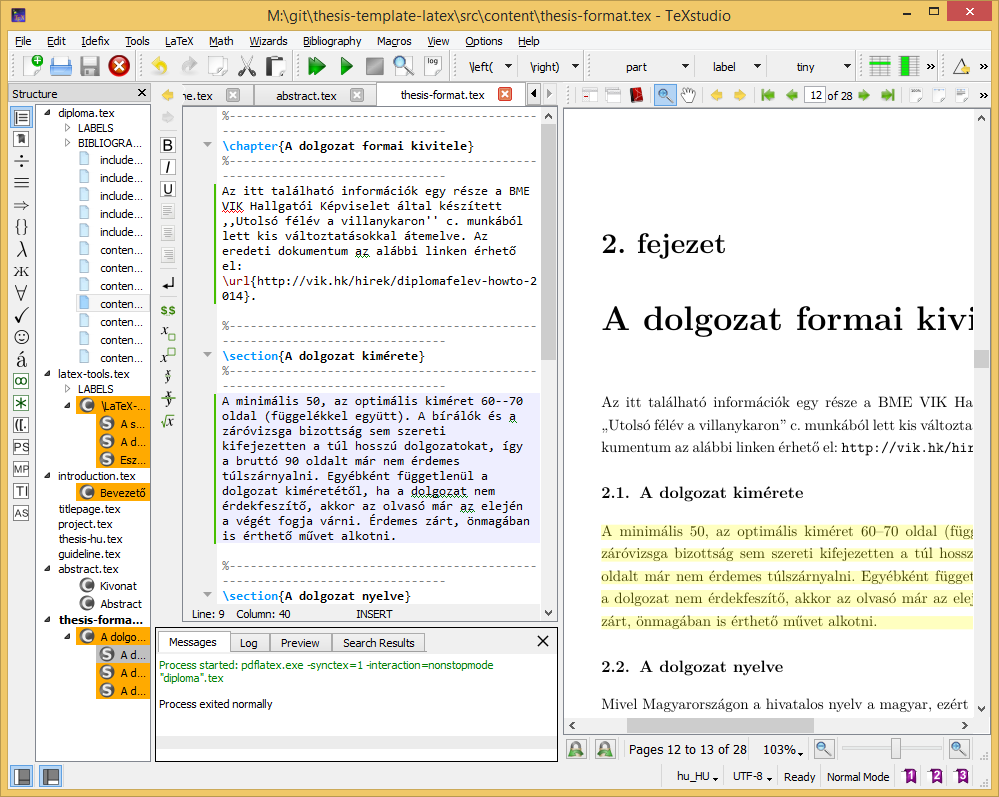
\includegraphics[width=67mm, keepaspectratio]{figures/TeXstudio.png}\hspace{1cm}
	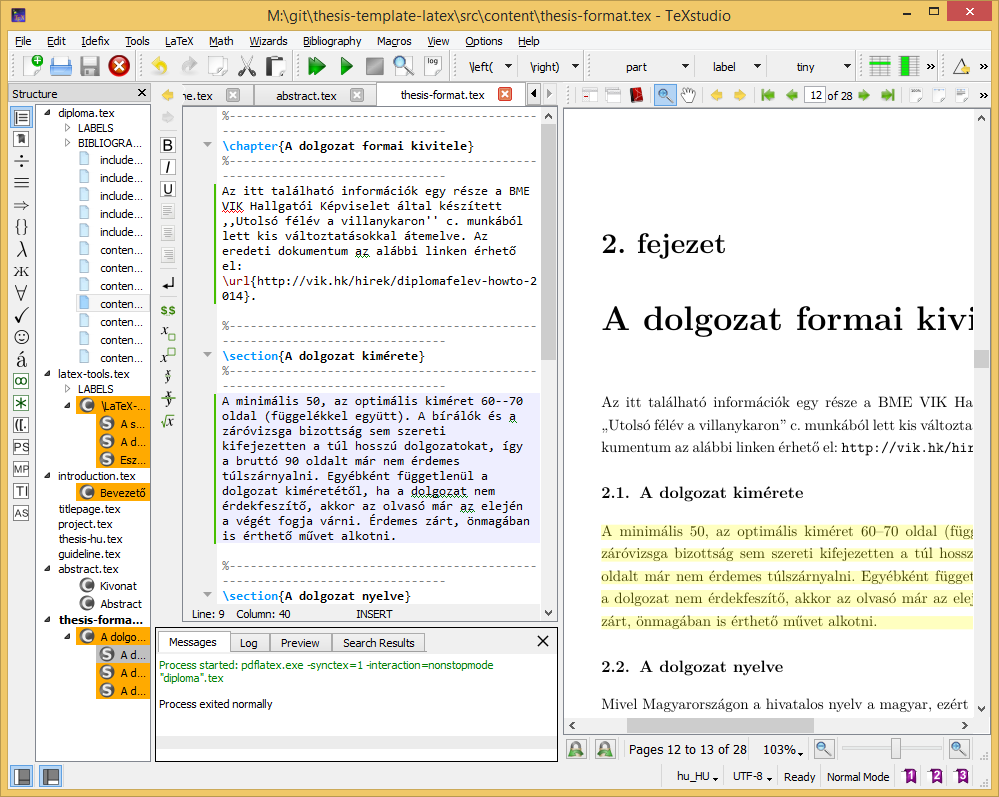
\includegraphics[width=67mm, keepaspectratio]{figures/TeXstudio.png}\\\vspace{5mm}
	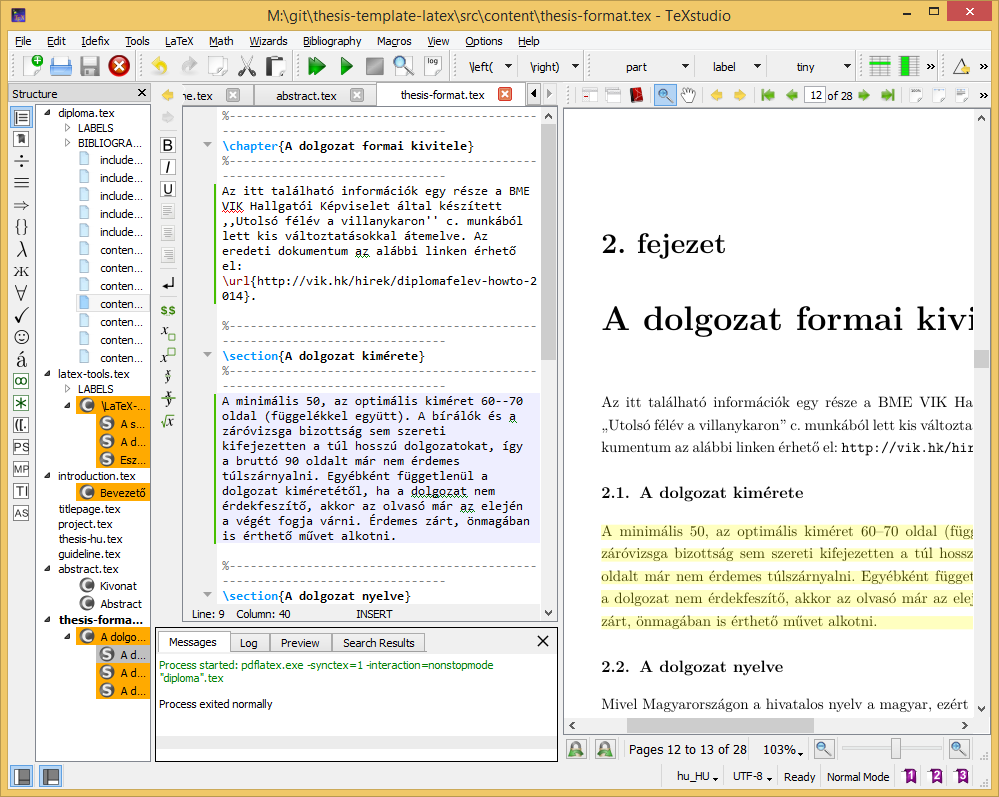
\includegraphics[width=67mm, keepaspectratio]{figures/TeXstudio.png}\hspace{1cm}
	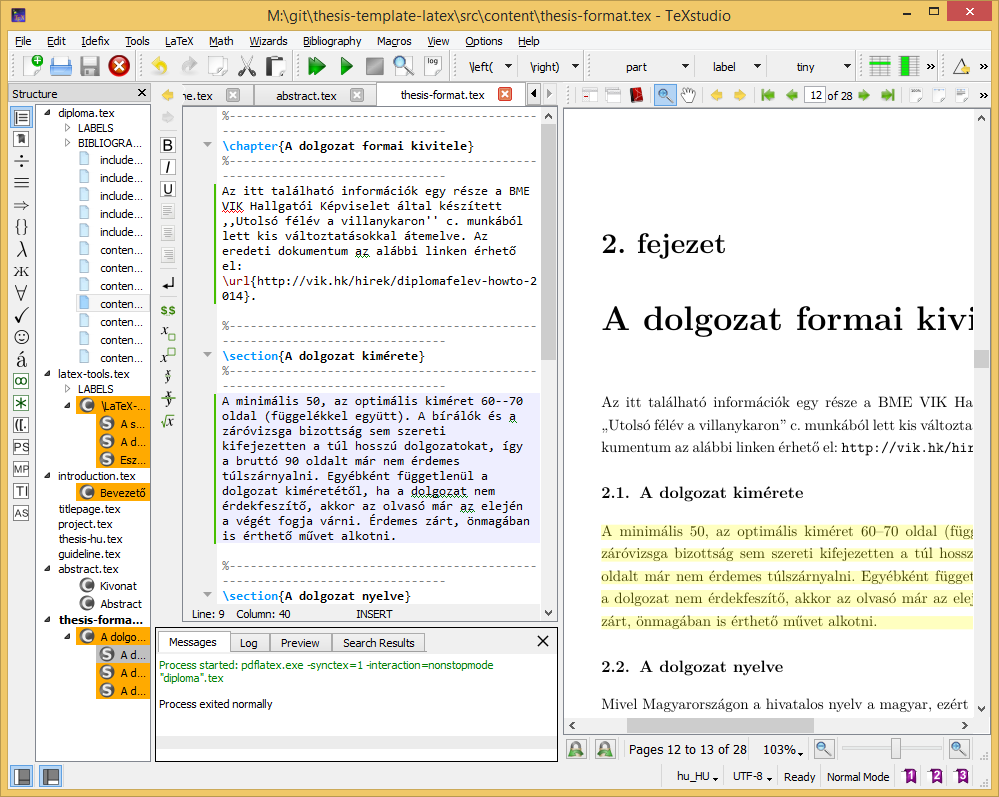
\includegraphics[width=67mm, keepaspectratio]{figures/TeXstudio.png}
	\caption{Több képfájl beillesztése esetén térközöket is érdemes használni.}
	\label{fig:HVSpaces}
\end{figure}

A táblázatok használatára \aref{tab:TabularExample}~táblázat mutat példát. A táblázatok formázásához hasznos tanácsokat találunk a \verb+booktabs+ csomag dokumentációjában.

\begin{table}[ht]
	\footnotesize
	\centering
	\begin{tabular}{ l c c }
		\toprule
		Órajel & Frekvencia & Cél pin \\
		\midrule
		CLKA & 100 MHz & FPGA CLK0\\
		CLKB & 48 MHz  & FPGA CLK1\\
		CLKC & 20 MHz  & Processzor\\
		CLKD & 25 MHz  & Ethernet chip \\
		CLKE & 72 MHz  & FPGA CLK2\\
		XBUF & 20 MHz  & FPGA CLK3\\
		\bottomrule
	\end{tabular}
	\caption{Az órajel-generátor chip órajel-kimenetei.}
	\label{tab:TabularExample}
\end{table}


%----------------------------------------------------------------------------
\section{Felsorolások és listák}
%----------------------------------------------------------------------------
Számozatlan felsorolásra mutat példát a jelenlegi bekezdés:
\begin{itemize}
	\item \emph{első bajusz:} ide lehetne írni az első elem kifejését,
	\item \emph{második bajusz:} ide lehetne írni a második elem kifejését,
	\item \emph{ez meg egy szakáll:} ide lehetne írni a harmadik elem kifejését.
\end{itemize}

Számozott felsorolást is készíthetünk az alábbi módon:
\begin{enumerate}
	\item \emph{első bajusz:} ide lehetne írni az első elem kifejését, és ez a kifejtés így néz ki, ha több sorosra sikeredik,
	\item \emph{második bajusz:} ide lehetne írni a második elem kifejését,
	\item \emph{ez meg egy szakáll:} ide lehetne írni a harmadik elem kifejését.
\end{enumerate}
A felsorolásokban sorok végén vessző, az utolsó sor végén pedig pont a szokásos írásjel. Ez alól kivételt képezhet, ha az egyes elemek több teljes mondatot tartalmaznak.

Listákban a dolgozat szövegétől elkülönítendő kódrészleteket, programsorokat, pszeudo-kódokat jeleníthetünk meg (\ref{lst:Example}.~kódrészlet).
\begin{lstlisting}[language=tex,caption=A fenti számozott felsorolás \LaTeX-forráskódja,label=lst:Example]
\begin{enumerate}
	\item \emph{els(*@ő@*) bajusz:} ide lehetne írni az els(*@ő@*) elem kifejését,
	és ez a kifejtés így néz ki, ha több sorosra sikeredik,
	\item \emph{második bajusz:} ide lehetne írni a második elem kifejését,
	\item \emph{ez meg egy szakáll:} ide lehetne írni a harmadik elem kifejését.
\end{enumerate}
\end{lstlisting}
A lista keretét, háttérszínét, egész stílusát megválaszthatjuk. Ráadásul különféle programnyelveket és a nyelveken belül kulcsszavakat is definiálhatunk, ha szükséges. Erről bővebbet a \verb+listings+ csomag hivatalos leírásában találhatunk.

%----------------------------------------------------------------------------
\section{Képletek}
%----------------------------------------------------------------------------
Ha egy formula nem túlságosan hosszú, és nem akarjuk hivatkozni a szövegből, mint például a $e^{i\pi}+1=0$ képlet, \emph{szövegközi képletként} szokás leírni. Csak, hogy másik példát is lássunk, az $U_i=-d\Phi/dt$ Faraday-törvény a $\rot E=-\frac{dB}{dt}$ differenciális alakban adott Maxwell-egyenlet felületre vett integráljából vezethető le. Látható, hogy a \LaTeX-fordító a sorközöket betartja, így a szöveg szedése esztétikus marad szövegközi képletek használata esetén is.

Képletek esetén az általános konvenció, hogy a kisbetűk skalárt, a kis félkövér betűk ($\mathbf{v}$) oszlopvektort -- és ennek megfelelően $\mathbf{v}^T$ sorvektort -- a kapitális félkövér betűk ($\mathbf{V}$) mátrixot jelölnek. Ha ettől el szeretnénk térni, akkor az alkalmazni kívánt jelölésmódot célszerű külön alfejezetben definiálni. Ennek megfelelően, amennyiben $\mathbf{y}$ jelöli a mérések vektorát, $\mathbf{\vartheta}$ a paraméterek vektorát és $\hat{\mathbf{y}}=\mathbf{X}\vartheta$ a paraméterekben lineáris modellt, akkor a \emph{Least-Squares} értelemben optimális paraméterbecslő $\hat{\mathbf{\vartheta}}_{LS}=(\mathbf{X}^T\mathbf{X})^{-1}\mathbf{X}^T\mathbf{y}$ lesz.

Emellett kiemelt, sorszámozott képleteket is megadhatunk, ennél az \verb+equation+ és a \verb+eqnarray+ környezetek helyett a korszerűbb \verb+align+ környezet alkalmazását javasoljuk (több okból, különféle problémák elkerülése végett, amelyekre most nem térünk ki). Tehát
\begin{align}
\dot{\mathbf{x}}&=\mathbf{A}\mathbf{x}+\mathbf{B}\mathbf{u},\\
\mathbf{y}&=\mathbf{C}\mathbf{x},
\end{align}
ahol $\mathbf{x}$ az állapotvektor, $\mathbf{y}$ a mérések vektora és $\mathbf{A}$, $\mathbf{B}$ és $\mathbf{C}$ a rendszert leíró paramétermátrixok. Figyeljük meg, hogy a két egyenletben az egyenlőségjelek egymáshoz igazítva jelennek meg, mivel a mindkettőt az \& karakter előzi meg a kódban. Lehetőség van számozatlan kiemelt képlet használatára is, például
\begin{align}
\dot{\mathbf{x}}&=\mathbf{A}\mathbf{x}+\mathbf{B}\mathbf{u},\nonumber\\
\mathbf{y}&=\mathbf{C}\mathbf{x}\nonumber.
\end{align}
Mátrixok felírására az $\mathbf{A}\mathbf{x}=\mathbf{b}$ inhomogén lineáris egyenlet részletes kifejtésével mutatunk példát:
\begin{align}
\begin{bmatrix}
a_{11} & a_{12} & \dots & a_{1n}\\
a_{21} & a_{22} & \dots & a_{2n}\\
\vdots & \vdots & \ddots & \vdots\\
a_{m1} & a_{m2} & \dots & a_{mn}
\end{bmatrix}
\begin{pmatrix}x_1\\x_2\\\vdots\\x_n\end{pmatrix}=
\begin{pmatrix}b_1\\b_2\\\vdots\\b_m\end{pmatrix}.
\end{align}
A \verb+\frac+ utasítás hatékonyságát egy általános másodfokú tag átviteli függvényén keresztül mutatjuk be, azaz
\begin{align}
W(s)=\frac{A}{1+2T\xi s+s^2T^2}.
\end{align}
A matematikai mód minden szimbólumának és képességének a bemutatására természetesen itt nincs lehetőség, de gyors referenciaként hatékonyan használhatók a következő linkek:\\
\indent\url{http://www.artofproblemsolving.com/LaTeX/AoPS_L_GuideSym.php},\\
\indent\url{http://www.ctan.org/tex-archive/info/symbols/comprehensive/symbols-a4.pdf},\\
\indent\url{ftp://ftp.ams.org/pub/tex/doc/amsmath/short-math-guide.pdf}.\\
Ez pedig itt egy magyarázat, hogy miért érdemes \verb+align+ környezetet használni:\\
\indent\url{http://texblog.net/latex-archive/maths/eqnarray-align-environment/}.

%----------------------------------------------------------------------------
\section{Irodalmi hivatkozások}
\label{sec:HowtoReference}
%----------------------------------------------------------------------------
Egy \LaTeX~dokumentumban az irodalmi hivatkozások definíciójának két módja van. Az egyik a \verb+\thebibliograhy+ környezet használata a dokumentum végén, az \verb+\end{document}+ lezárás előtt.
\begin{lstlisting}[language=tex]
\begin{thebibliography}{9}

\bibitem{Lamport94} Leslie Lamport, \emph{\LaTeX: A Document Preparation System}.
Addison Wesley, Massachusetts, 2nd Edition, 1994.

\end{thebibliography}
\end{lstlisting}

Ezek után a dokumentumban a \verb+\cite{Lamport94}+ utasítással hivatkozhatunk a forrásra. A fenti megadás viszonylag kötetlen, a szerző maga formázza az irodalomjegyzéket (ami gyakran inkonzisztens eredményhez vezet).

Egy sokkal professzionálisabb módszer a BiB\TeX{} használata, ezért ez a sablon is ezt támogatja. Ebben az esetben egy külön szöveges adatbázisban definiáljuk a forrásmunkákat, és egy külön stílusfájl határozza meg az irodalomjegyzék kinézetét. Ez, összhangban azzal, hogy külön formátumkonvenció határozza meg a folyóirat-, a könyv-, a konferenciacikk- stb. hivatkozások kinézetét az irodalomjegyzékben (a sablon használata esetén ezzel nem is kell foglalkoznia a hallgatónak, de az eredményt célszerű ellenőrizni). felhasznált hivatkozások adatbázisa egy \verb+.bib+ kiterjesztésű szöveges fájl, amelynek szerkezetét a \Aref{lst:Bibtex} kódrészlet demonstrálja. A forrásmunkák bevitelekor a sor végi vesszők külön figyelmet igényelnek, mert hiányuk a BiB\TeX-fordító hibaüzenetét eredményezi. A forrásmunkákat típus szerinti kulcsszó vezeti be (\verb+@book+ könyv, \verb+@inproceedings+ konferenciakiadványban megjelent cikk, \verb+@article+ folyóiratban megjelent cikk, \verb+@techreport+ valamelyik egyetem gondozásában megjelent műszaki tanulmány, \verb+@manual+ műszaki dokumentáció esetén stb.). Nemcsak a megjelenés stílusa, de a kötelezően megadandó mezők is típusról-típusra változnak. Egy jól használható referencia a \url{http://en.wikipedia.org/wiki/BibTeX} oldalon található.

\begin{lstlisting}[caption=Példa szöveges irodalomjegyzék-adatbázisra Bib\TeX{} használata esetén.,label=lst:Bibtex]
@book{Wettl04,
  author    = {Ferenc Wettl and Gyula Mayer and Péter Szabó},
  publisher = {Panem Könyvkiadó},
  title     = {\LaTeX~kézikönyv},
  year      = {2004},
}

@article{Candy86,
  author       = {James C. Candy},
  journaltitle = {{IEEE} Trans.\ on Communications},
  month        = {01},
  note         = {\doi{10.1109/TCOM.1986.1096432}},
  number       = {1},
  pages        = {72--76},
  title        = {Decimation for Sigma Delta Modulation},
  volume       = {34},
  year         = {1986},
}

@inproceedings{Lee87,
  author    = {Wai L. Lee and Charles G. Sodini},
  booktitle = {Proc.\ of the IEEE International Symposium on Circuits and Systems},
  location  = {Philadelphia, PA, USA},
  month     = {05~4--7},
  pages     = {459--462},
  title     = {A Topology for Higher Order Interpolative Coders},
  vol       = {2},
  year      = {1987},
}

@thesis{KissPhD,
  author      = {Peter Kiss},
  institution = {Technical University of Timi\c{s}oara, Romania},
  month       = {04},
  title       = {Adaptive Digital Compensation of Analog Circuit Imperfections for Cascaded Delta-Sigma Analog-to-Digital Converters},
  type        = {phdthesis},
  year        = {2000},
}

@manual{Schreier00,
  author       = {Richard Schreier},
  month        = {01},
  note         = {\url{http://www.mathworks.com/matlabcentral/fileexchange/}},
  organization = {Oregon State University},
  title        = {The Delta-Sigma Toolbox v5.2},
  year         = {2000},
}

@misc{DipPortal,
  author       = {{Budapesti Műszaki és Gazdaságtudományi Egyetem Villamosmérnöki és Informatikai Kar}},
  howpublished = {\url{http://diplomaterv.vik.bme.hu/}},
  title        = {Diplomaterv portál (2011. február 26.)},
}

@incollection{Mkrtychev:1997,
  author    = {Mkrtychev, Alexey},
  booktitle = {Logical Foundations of Computer Science},
  doi       = {10.1007/3-540-63045-7_27},
  editor    = {Adian, Sergei and Nerode, Anil},
  isbn      = {978-3-540-63045-6},
  pages     = {266-275},
  publisher = {Springer Berlin Heidelberg},
  series    = {Lecture Notes in Computer Science},
  title     = {Models for the logic of proofs},
  url       = {http://dx.doi.org/10.1007/3-540-63045-7_27},
  volume    = {1234},
  year      = {1997},
}
\end{lstlisting}

A stílusfájl egy \verb+.sty+ kiterjesztésű fájl, de ezzel lényegében nem kell foglalkozni, mert vannak beépített stílusok, amelyek jól használhatók. Ez a sablon a BiB\TeX-et használja, a hozzá tartozó adatbázisfájl a \verb+mybib.bib+ fájl. Megfigyelhető, hogy az irodalomjegyzéket a dokumentum végére (a \verb+\end{document}+ utasítás elé) beillesztett \verb+\bibliography{mybib}+ utasítással hozhatjuk létre, a stílusát pedig ugyanitt a  \verb+\bibliographystyle{plain}+ utasítással adhatjuk meg. Ebben az esetben a \verb+plain+ előre definiált stílust használjuk (a sablonban is ezt állítottuk be). A \verb+plain+ stíluson kívül természetesen számtalan más előre definiált stílus is létezik. Mivel a \verb+.bib+ adatbázisban ezeket megadtuk, a BiB\TeX-fordító is meg tudja különböztetni a szerzőt a címtől és a kiadótól, és ez alapján automatikusan generálódik az irodalomjegyzék a stílusfájl által meghatározott stílusban.

Az egyes forrásmunkákra a szövegből továbbra is a \verb+\cite+ paranccsal tudunk hivatkozni, így \aref{lst:Bibtex}.~kódrészlet esetén a hivatkozások rendre \verb+\cite{Wettl04}+, \verb+\cite{Candy86}+, \verb+\cite{Lee87}+, \verb+\cite{KissPhD}+, \verb+\cite{Schreirer00}+,
\verb+\cite{Mkrtychev:1997}+ és \verb+\cite{DipPortal}+. Az egyes forrásmunkák sorszáma az irodalomjegyzék bővítésekor változhat. Amennyiben az aktuális számhoz illeszkedő névelőt szeretnénk használni, használjuk az \verb+\acite{}+ parancsot.

Az irodalomjegyzékben alapértelmezésben csak azok a forrásmunkák jelennek meg, amelyekre található hivatkozás a szövegben, és ez így alapvetően helyes is, hiszen olyan forrásmunkákat nem illik az irodalomjegyzékbe írni, amelyekre nincs hivatkozás.

Mivel a fordítási folyamat során több lépésben oldódnak fel a szimbólumok, ezért gyakran többször is le kell fordítani a dokumentumot. Ilyenkor ez első 1-2 fordítás esetleg szimbólum-feloldásra vonatkozó figyelmeztető üzenettel zárul. Ha hibaüzenettel zárul bármelyik fordítás, akkor nincs értelme megismételni, hanem a hibát kell megkeresni. A \verb+.bib+ fájl megváltoztatáskor sokszor nincs hatása a változtatásnak azonnal, mivel nem mindig fut újra a BibTeX fordító. Ezért célszerű a változtatás után azt manuálisan is lefuttatni (TeXstudio esetén \verb+Tools/Bibliography+).

Hogy a szövegbe ágyazott hivatkozások kinézetét demonstráljuk, itt most sorban meghivatkozzuk a \cite{Wettl04}, \cite{Candy86}, \cite{Lee87}, \cite{KissPhD}, \cite{Schreier00} és \acite{Mkrtychev:1997}\footnote{Informatikai témában gyakran hivatkozunk cikkeket a Springer LNCS valamely kötetéből, ez a hivatkozás erre mutat egy helyes példát.} forrásmunkát, valamint \acite{DipPortal} weboldalt.

Megjegyzendő, hogy az ékezetes magyar betűket is tartalmazó \verb+.bib+ fájl az \verb+inputenc+ csomaggal betöltött \verb+latin2+ betűkészlet miatt fordítható. Ugyanez a \verb+.bib+ fájl hibaüzenettel fordul egy olyan dokumentumban, ami nem tartalmazza a \verb+\usepackage[latin2]{inputenc}+ sort. Speciális igény esetén az irodalmi adatbázis általánosabb érvényűvé tehető, ha az ékezetes betűket speciális latex karakterekkel helyettesítjük a \verb+.bib+ fájlban, pl. á helyett \verb+\'{a}+-t vagy ő helyett \verb+\H{o}+-t írunk.

Irodalomhivatkozásokat célszerű először olyan szolgáltatásokban keresni, ahol jó minőségű bejegyzések találhatók (pl. ACM Digital Library,\footnote{\url{https://dl.acm.org/}} DBLP,\footnote{\url{http://dblp.uni-trier.de/}} IEEE Xplore,\footnote{\url{http://ieeexplore.ieee.org/}} SpringerLink\footnote{\url{https://link.springer.com/}}) és csak ezek után használni kevésbé válogatott forrásokat (pl. Google Scholar\footnote{\url{http://scholar.google.com/}}). A jó minőségű bejegyzéseket is érdemes megfelelően tisztítani.\footnote{\url{https://github.com/FTSRG/cheat-sheets/wiki/BibTeX-Fixing-entries-from-common-sources}} A sablon angol nyelvű változatában használt \texttt{plainnat} beállítás egyik sajátossága, hogy a cikkhez generált hivatkozás a cikk DOI-ját és URL-jét is tartalmazza, ami gyakran duplikátumhoz vezet -- érdemes tehát a DOI-kat tartalmazó URL mezőket törölni. 

%----------------------------------------------------------------------------
\section{A dolgozat szerkezete és a forrásfájlok}
%----------------------------------------------------------------------------
A diplomatervsablonban a TeX fájlok két alkönyvtárban helyezkednek el. Az \verb+include+ könyvtárban azok szerepelnek, amiket tipikusan nem kell szerkesztenünk, ezek a sablon részei (pl. címoldal). A \verb+content+ alkönyvtárban pedig a saját munkánkat helyezhetjük el. Itt érdemes az egyes fejezeteket külön \TeX{} állományokba rakni.

A diplomatervsablon (a kari irányelvek szerint) az alábbi fő fejezetekből áll:
\begin{enumerate}
	\item 1 oldalas \emph{tájékoztató} a szakdolgozat/diplomaterv szerkezetéről (\verb+include/guideline.tex+), ami a végső dolgozatból törlendő,
	\item \emph{feladatkiírás} (\verb+include/project.tex+), a dolgozat nyomtatott verzójában ennek a helyére kerül a tanszék által kiadott, a tanszékvezető által aláírt feladatkiírás, a dolgozat elektronikus verziójába pedig a feladatkiírás egyáltalán ne kerüljön bele, azt külön tölti fel a tanszék a diplomaterv-honlapra,
	\item \emph{címoldal} (\verb+include/titlepage.tex+),
	\item \emph{tartalomjegyzék} (\verb+thesis.tex+),
	\item a diplomatervező \emph{nyilatkozat}a az önálló munkáról (\verb+include/declaration.tex+),
	\item 1-2 oldalas tartalmi \emph{összefoglaló} magyarul és angolul, illetve elkészíthető még további nyelveken is (\verb+content/abstract.tex+),
	\item \emph{bevezetés}: a feladat értelmezése, a tervezés célja, a feladat indokoltsága, a diplomaterv felépítésének rövid összefoglalása (\verb+content/introduction.tex+),
	\item sorszámmal ellátott \emph{fejezetek}: a feladatkiírás pontosítása és részletes elemzése, előzmények (irodalomkutatás, hasonló alkotások), az ezekből levonható következtetések, a tervezés részletes leírása, a döntési lehetőségek értékelése és a választott megoldások indoklása, a megtervezett műszaki alkotás értékelése, kritikai elemzése, továbbfejlesztési lehetőségek,
	\item esetleges \emph{köszönetnyilvánítás}ok (\verb+content/acknowledgement.tex+),
	\item részletes és pontos \emph{irodalomjegyzék} (ez a sablon esetében automatikusan generálódik a \verb+thesis.tex+ fájlban elhelyezett \verb+\bibliography+ utasítás hatására, \az+\refstruc{sec:HowtoReference}ban leírtak szerint),
	\item \emph{függelékek} (\verb+content/appendices.tex+).
\end{enumerate}

A sablonban a fejezetek a \verb+thesis.tex+ fájlba vannak beillesztve \verb+\include+ utasítások segítségével. Lehetőség van arra, hogy csak az éppen szerkesztés alatt álló \verb+.tex+ fájlt fordítsuk le, ezzel lerövidítve a fordítási folyamatot. Ezt a lehetőséget az alábbi kódrészlet biztosítja a \verb+thesis.tex+ fájlban.
\begin{lstlisting}
\includeonly{
	guideline,%
	project,%
	titlepage,%
	declaration,%
	abstract,%
	introduction,%
	chapter1,%
	chapter2,%
	chapter3,%
	acknowledgement,%
	appendices,%
}
\end{lstlisting}

Ha az alábbi kódrészletben az egyes sorokat a \verb+%+ szimbólummal kikommentezzük, akkor a megfelelő \verb+.tex+ fájl nem fordul le. Az oldalszámok és a tartalomjegyék természetesen csak akkor billennek helyre, ha a teljes dokumentumot lefordítjuk.

%----------------------------------------------------------------------------
\newpage
\section{Alapadatok megadása}
%----------------------------------------------------------------------------
A diplomaterv alapadatait (cím, szerző, konzulens, konzulens titulusa) a \verb+thesis.tex+ fájlban lehet megadni.

%----------------------------------------------------------------------------
\section{Új fejezet írása}
%----------------------------------------------------------------------------
A főfejezetek külön \verb+content+ könyvtárban foglalnak helyet. A sablonhoz 3 fejezet készült. További főfejezeteket úgy hozhatunk létre, ha új \TeX~fájlt készítünk a fejezet számára, és a \verb+thesis.tex+ fájlban, a \verb+\include+ és \verb+\includeonly+ utasítások argumentumába felvesszük az új \verb+.tex+ fájl nevét.


%----------------------------------------------------------------------------
\section{Definíciók, tételek, példák}
%----------------------------------------------------------------------------

\begin{definition}[Fluxuskondenzátor térerőssége]
Lorem ipsum dolor sit amet, consectetur adipiscing elit, sed do eiusmod tempor incididunt ut labore et dolore magna aliqua. Ut enim ad minim veniam, quis nostrud exercitation ullamco laboris nisi ut aliquip ex ea commodo consequat.
\end{definition}

\begin{example}
Példa egy példára. Duis aute irure dolor in reprehenderit in voluptate velit esse cillum dolore eu fugiat nulla pariatur. Excepteur sint occaecat cupidatat non proident, sunt in culpa qui officia deserunt mollit anim id est laborum.
\end{example}

\begin{theorem}[Kovács tétele]
Duis aute irure dolor in reprehenderit in voluptate velit esse cillum dolore eu fugiat nulla pariatur. Excepteur sint occaecat cupidatat non proident, sunt in culpa qui officia deserunt mollit anim id est laborum.
\end{theorem}



% Acknowledgements
%~~~~~~~~~~~~~~~~~~~~~~~~~~~~~~~~~~~~~~~~~~~~~~~~~~~~~~~~~~~~~~~~~~~~~~~~~~~~~~~~~~~~~~
%\chapter{Acknowledgement} \label{acknowledgements}

I would like to thank and give my best regards to my supervisors, Gábor Sörös and Judit Tevesz for their valuable insights throughout the development of this thesis. Their encouragement and expert advice have been invaluable in overcoming challenges and achieving my goals.

I wish to thank Nokia Bell Labs for providing me the opportunity to work on their mobile robot and for lending me an OAK-D camera with which I could experiment and implement my features at home.

My sincere thanks also go to the Spectacular AI Team, particularly Jerry Ylilammi for generously providing access to their SDK for the Raspberry Pi 4 for educational purposes. Their support allowed me to explore advanced technologies and implement key components of this project.



% List of Figures, Tables
%~~~~~~~~~~~~~~~~~~~~~~~~~~~~~~~~~~~~~~~~~~~~~~~~~~~~~~~~~~~~~~~~~~~~~~~~~~~~~~~~~~~~~~
%\listoffigures\addcontentsline{toc}{chapter}{\listfigurename}
%\listoftables\addcontentsline{toc}{chapter}{\listtablename}


% Bibliography
%~~~~~~~~~~~~~~~~~~~~~~~~~~~~~~~~~~~~~~~~~~~~~~~~~~~~~~~~~~~~~~~~~~~~~~~~~~~~~~~~~~~~~~
\addcontentsline{toc}{chapter}{\bibname}
\bibliography{bib/mybib}


% Appendix
%~~~~~~~~~~~~~~~~~~~~~~~~~~~~~~~~~~~~~~~~~~~~~~~~~~~~~~~~~~~~~~~~~~~~~~~~~~~~~~~~~~~~~~
%----------------------------------------------------------------------------
\appendix
%----------------------------------------------------------------------------
\chapter*{\fuggelek}\addcontentsline{toc}{chapter}{\fuggelek}
\setcounter{chapter}{\appendixnumber}
%\setcounter{equation}{0} % a fofejezet-szamlalo az angol ABC 6. betuje (F) lesz
\numberwithin{equation}{section}
\numberwithin{figure}{section}
\numberwithin{lstlisting}{section}
%\numberwithin{tabular}{section}


\section{RTAB-Map custom launch file} \label{rtabmap_custom_launch_file}
\begin{lstlisting}[language=python,frame=single]
"""Custom launch file for rtabmap.

Launches:

 - RTAB-Map
 - RTAB-Map visualizer

To use launch also:

 - ``camera.launch.py`` from ``depthai_ros_driver`` package
"""
import os

from ament_index_python.packages import get_package_share_directory
from launch import LaunchDescription
from launch.actions import DeclareLaunchArgument, IncludeLaunchDescription, OpaqueFunction
from launch.conditions import IfCondition
from launch.launch_description_sources import PythonLaunchDescriptionSource
from launch.substitutions import LaunchConfiguration
from launch_ros.actions import LoadComposableNodes, Node
from launch_ros.descriptions import ComposableNode

def launch_setup(context, *args, **kwargs):
    name = LaunchConfiguration('name').perform(context)
    depthai_prefix = get_package_share_directory("depthai_ros_driver")

    params_file= LaunchConfiguration("params_file")
    parameters = [
        {
            "frame_id": name,
            "subscribe_rgb": True,
            "subscribe_depth": True,
            "subscribe_odom_info": True,
            "approx_sync": True,
            "Rtabmap/DetectionRate": "3.5",
        }
    ]

    remappings = [
        ("rgb/image", name+"/rgb/image_rect"),
        ("rgb/camera_info", name+"/rgb/camera_info"),
        ("depth/image", name+"/stereo/image_raw"),
    ]

    return [
        LoadComposableNodes(
            condition=IfCondition(LaunchConfiguration("rectify_rgb")),
            target_container=name+"_container",
            composable_node_descriptions=[
                ComposableNode(
                    package="image_proc",
                    plugin="image_proc::RectifyNode",
                    name="rectify_color_node",
                    remappings=[('image', name+'/rgb/image_raw'),
                                ('camera_info', name+'/rgb/camera_info'),
                                ('image_rect', name+'/rgb/image_rect'),
                                ('image_rect/compressed', name+'/rgb/image_rect/compressed'),
                                ('image_rect/compressedDepth', name+'/rgb/image_rect/compressedDepth'),
                                ('image_rect/theora', name+'/rgb/image_rect/theora')]
                )
            ]),
        
        LoadComposableNodes(
            target_container=name+"_container",
            composable_node_descriptions=[
                ComposableNode(
                    package='rtabmap_odom',
                    plugin='rtabmap_odom::RGBDOdometry',
                    name='rgbd_odometry',
                    parameters=parameters,
                    remappings=remappings,
                ),
            ],
        ),

        LoadComposableNodes(
            target_container=name+"_container",
            composable_node_descriptions=[
                ComposableNode(
                    package='rtabmap_slam',
                    plugin='rtabmap_slam::CoreWrapper',
                    name='rtabmap',
                    parameters=parameters,
                    remappings=remappings,
                ),
            ],
        ),

        Node(
            package="rtabmap_viz",
            executable="rtabmap_viz",
            output="screen",
            parameters=parameters,
            remappings=remappings,
        ),
    ]


def generate_launch_description():
    depthai_prefix = get_package_share_directory("depthai_ros_driver")
    declared_arguments = [
        DeclareLaunchArgument("name", default_value="oak"),
        DeclareLaunchArgument("params_file", default_value=os.path.join(depthai_prefix, 'config', 'rgbd.yaml')),
        DeclareLaunchArgument("rectify_rgb", default_value="True"),
    ]

    return LaunchDescription(
        declared_arguments + [OpaqueFunction(function=launch_setup)]
    )

\end{lstlisting}

\section{Custom person detector code} \label{custom_person_detector}

\begin{lstlisting}[language=python,frame=single]
"""Person detection with OAK-D and ROS2

The script uses an OAK-D camera and Spectacular AI to detect
persons and then a ROS2 Node publishes its position
relative to the camera onto the ``/detected_persons`` topic.

Positions:

 - X: distance from camera
 - Y: horizontal position
 - Z: vertical position
"""
import depthai as dai
import time
import cv2
import matplotlib.pyplot as plt
import spectacularAI
import threading
from pathlib import Path
import sys
import numpy as np
import rclpy
from rclpy.node import Node
from geometry_msgs.msg import Point


class PersonDetectorNode(Node):

    def __init__(self):
        super().__init__('person_detector')
        self.publisher_ = self.create_publisher(Point, 'detected_persons', 10)

def make_pipelines(nnBlobPath, showRgb):
    syncNN = True

    # Create pipeline
    pipeline = dai.Pipeline()
    vio_pipeline = spectacularAI.depthai.Pipeline(pipeline)
    spatialCalc = pipeline.create(dai.node.SpatialLocationCalculator)

    # Define sources and outputs
    camRgb = pipeline.createColorCamera()
    spatialDetectionNetwork = pipeline.createYoloSpatialDetectionNetwork()

    if showRgb:
        xoutRgb = pipeline.createXLinkOut()
    xoutNN = pipeline.createXLinkOut()
    xoutBoundingBoxDepthMapping = pipeline.createXLinkOut()

    if showRgb:
        xoutRgb.setStreamName("rgb")
    xoutNN.setStreamName("detections")
    xoutBoundingBoxDepthMapping.setStreamName("boundingBoxDepthMapping")

    # Properties
    camRgb.setPreviewSize(416, 416)
    camRgb.setResolution(dai.ColorCameraProperties.SensorResolution.THE_1080_P)
    camRgb.setInterleaved(False)
    camRgb.setColorOrder(dai.ColorCameraProperties.ColorOrder.BGR)

    spatialDetectionNetwork.setBlobPath(nnBlobPath)
    spatialDetectionNetwork.setConfidenceThreshold(0.5)
    spatialDetectionNetwork.input.setBlocking(False)
    spatialDetectionNetwork.setBoundingBoxScaleFactor(0.5)
    spatialDetectionNetwork.setDepthLowerThreshold(100)
    spatialDetectionNetwork.setDepthUpperThreshold(5000)

    # Yolo specific parameters
    spatialDetectionNetwork.setNumClasses(80)
    spatialDetectionNetwork.setCoordinateSize(4)
    spatialDetectionNetwork.setAnchors(np.array([10,14, 23,27, 37,58, 81,82, 135,169, 344,319]))
    spatialDetectionNetwork.setAnchorMasks({ "side26": np.array([1,2,3]), "side13": np.array([3,4,5]) })
    spatialDetectionNetwork.setIouThreshold(0.5)

    camRgb.preview.link(spatialDetectionNetwork.input)
    if showRgb:
        if syncNN:
            spatialDetectionNetwork.passthrough.link(xoutRgb.input)
        else:
            camRgb.preview.link(xoutRgb.input)

    spatialDetectionNetwork.out.link(xoutNN.input)
    spatialDetectionNetwork.boundingBoxMapping.link(xoutBoundingBoxDepthMapping.input)

    vio_pipeline.stereo.depth.link(spatialDetectionNetwork.inputDepth)

    return pipeline, vio_pipeline, spatialCalc

def make_tracker():
    """
    Simple tracker/smoother/clustring for the YOLO-detected objects.
    (The raw YOLO results look quite, well, raw, especially in 3D)
    """
    tracked_objects = []
    next_id = 1

    class TrackedObject:
        def __init__(self, t, p, l):
            self.position = p
            self.label = l
            self.last_seen = t
            self.n_detections = 1

            nonlocal next_id
            self.id = next_id
            next_id += 1

        def update(self, other):
            UPDATE_ALPHA = 0.2
            self.last_seen = other.last_seen
            self.position = UPDATE_ALPHA * other.position + (1.0 - UPDATE_ALPHA) * self.position
            self.n_detections += 1

        def __repr__(self):
            return '%s %d' % (self.label, self.id)

    CLUSTERING_DISTANCE_AT_1M = 0.3

    def find_best_match(new_obj, w_to_c_mat):
        best = None
        best_dist = CLUSTERING_DISTANCE_AT_1M
        MIN_DEPTH = 0.5

        local_pos = lambda p: (w_to_c_mat @ np.array(list(p) + [1]))[:3]

        for old in tracked_objects:
            if old.label != new_obj.label: continue

            # ignore depth difference in clustering
            loc_old = local_pos(old.position)
            loc_new = local_pos(new_obj.position)
            z = max([MIN_DEPTH, loc_old[2], loc_new[2]])
            dist = np.linalg.norm((loc_old - loc_new)[:2]) / z

            if dist < best_dist:
                best_dist = dist
                best = old
        # if best: print(f'matched with {best} (seen {best.n_detections} time(s))')
        return best

    def track(t, detections, view_mat):
        SCALE = 0.001 # output is millimeters
        MIN_DETECTIONS = 8
        DETECTION_WINDOW = 1.0
        MAX_UNSEEN_AGE = 8.0

        w_to_c_mat = np.linalg.inv(view_mat)

        for d in detections:
            p_local = np.array([
                d.spatialCoordinates.x * SCALE,
                -d.spatialCoordinates.y * SCALE, # note: flipped y
                d.spatialCoordinates.z * SCALE,
                1
            ])
            p_world = (view_mat @ p_local)[:3]
            try:
                label = LABEL_MAP[d.label]
            except:
                label = d.label

            # simple O(n^2)
            for o in tracked_objects:
                if o.label != label: continue
                dist = np.linalg.norm(o.position - p_world)

            if label in SELECTED_LABELS:
                new_obj = TrackedObject(t, p_world, label)
                existing = find_best_match(new_obj, w_to_c_mat)
                if existing:
                    existing.update(new_obj)
                else:
                    tracked_objects.append(new_obj)

        def should_remove(o):
            if o.n_detections < MIN_DETECTIONS and o.last_seen < t - DETECTION_WINDOW: return True
            if o.last_seen < t - MAX_UNSEEN_AGE: return True
            return False

        # remove cruft
        i = 0
        while i < len(tracked_objects):
            if should_remove(tracked_objects[i]):
                # print(f'removing ${o}')
                del tracked_objects[i]
            else:
                i += 1

        # print(tracked_objects)
        return [o for o in tracked_objects if o.n_detections >= MIN_DETECTIONS]

    return track

# Tiny yolo v3/4 label texts
LABEL_MAP = [
    "person",         "bicycle",    "car",           "motorbike",     "aeroplane",   "bus",           "train",
    "truck",          "boat",       "traffic light", "fire hydrant",  "stop sign",   "parking meter", "bench",
    "bird",           "cat",        "dog",           "horse",         "sheep",       "cow",           "elephant",
    "bear",           "zebra",      "giraffe",       "backpack",      "umbrella",    "handbag",       "tie",
    "suitcase",       "frisbee",    "skis",          "snowboard",     "sports ball", "kite",          "baseball bat",
    "baseball glove", "skateboard", "surfboard",     "tennis racket", "bottle",      "wine glass",    "cup",
    "fork",           "knife",      "spoon",         "bowl",          "banana",      "apple",         "sandwich",
    "orange",         "broccoli",   "carrot",        "hot dog",       "pizza",       "donut",         "cake",
    "chair",          "sofa",       "pottedplant",   "bed",           "diningtable", "toilet",        "tvmonitor",
    "laptop",         "mouse",      "remote",        "keyboard",      "cell phone",  "microwave",     "oven",
    "toaster",        "sink",       "refrigerator",  "book",          "clock",       "vase",          "scissors",
    "teddy bear",     "hair drier", "toothbrush"
]

SELECTED_LABELS = ['person']

if __name__ == '__main__':
    rclpy.init()
    nnBlobPath = 'models/yolo-v4-tiny-tf_openvino_2021.4_6shave.blob'
    if len(sys.argv) > 1:
        nnBlobPath = sys.argv[1]

    if not Path(nnBlobPath).exists():
        raise FileNotFoundError(f'Could not find {nnBlobPath}"')

    showRgb = True
    pipeline, vio_pipeline, spatialCalc = make_pipelines(nnBlobPath, showRgb)

    with dai.Device(pipeline) as device:

        detector_node = PersonDetectorNode()

        def main_loop():
            startTime = time.monotonic()
            counter = 0
            fps = 0
            color = (255, 255, 255)

            vio_session = vio_pipeline.startSession(device)
            tracker = make_tracker()

            # If I delete the following line the camera just throws this:
            # SpectacularAI WARN: IMU buffer max size exceeded, not waiting for more frames
            # and it freezes
            if showRgb: previewQueue = device.getOutputQueue(name="rgb", maxSize=4, blocking=False)
            
            detectionNNQueue = device.getOutputQueue(name="detections", maxSize=4, blocking=False)

            vio_matrix = None

            while True:
                if vio_session.hasOutput():
                    vio_out = vio_session.getOutput()
                    vio_matrix = vio_out.pose.asMatrix()
                elif detectionNNQueue.has():
                    
                    inDet = detectionNNQueue.get()

                    counter+=1
                    current_time = time.monotonic()
                    if (current_time - startTime) > 1 :
                        fps = counter / (current_time - startTime)
                        counter = 0
                        startTime = current_time


                    detections = inDet.detections

                    msg = Point()

                    if vio_matrix is not None:
                        detections_world = tracker(current_time, detections, vio_matrix)
                        
                        for detection in detections_world:
                             msg.x = detection.position[0] # distance from camera
                             msg.y = detection.position[1] # horizontal
                             msg.z = detection.position[2] # vertical

                             detector_node.publisher_.publish(msg)                        
                else:
                    time.sleep(0.005)

            vio_session.close()

        main_loop()
        
\end{lstlisting}

%\label{page:last}
\end{document}
